\documentclass[10pt, oneside]{article} % The default font size and one-sided printing (no margin offsets)

\usepackage[spanish]{babel}
\usepackage{subfig}
\usepackage{titlesec}
\usepackage{array}
\usepackage{graphicx}
\usepackage{float}
\usepackage{listings}
\usepackage{caption}
\newcolumntype{L}[1]{>{\raggedright\let\newline\\\arraybackslash\hspace{0pt}}m{#1}}
\newcolumntype{C}[1]{>{\centering\let\newline\\\arraybackslash\hspace{0pt}}m{#1}}
\newcolumntype{R}[1]{>{\raggedleft\let\newline\\\arraybackslash\hspace{0pt}}m{#1}}

\begin{document}
 
\section{Faltantes}

Muestra condiciones de frontera libres, graficar usando ovito's atomic strain.
 
\section{CuZr a distintas temperaturas}

%
%	Compresion
%

\subsection{Compresion}

\begin{figure}[H]
\centering
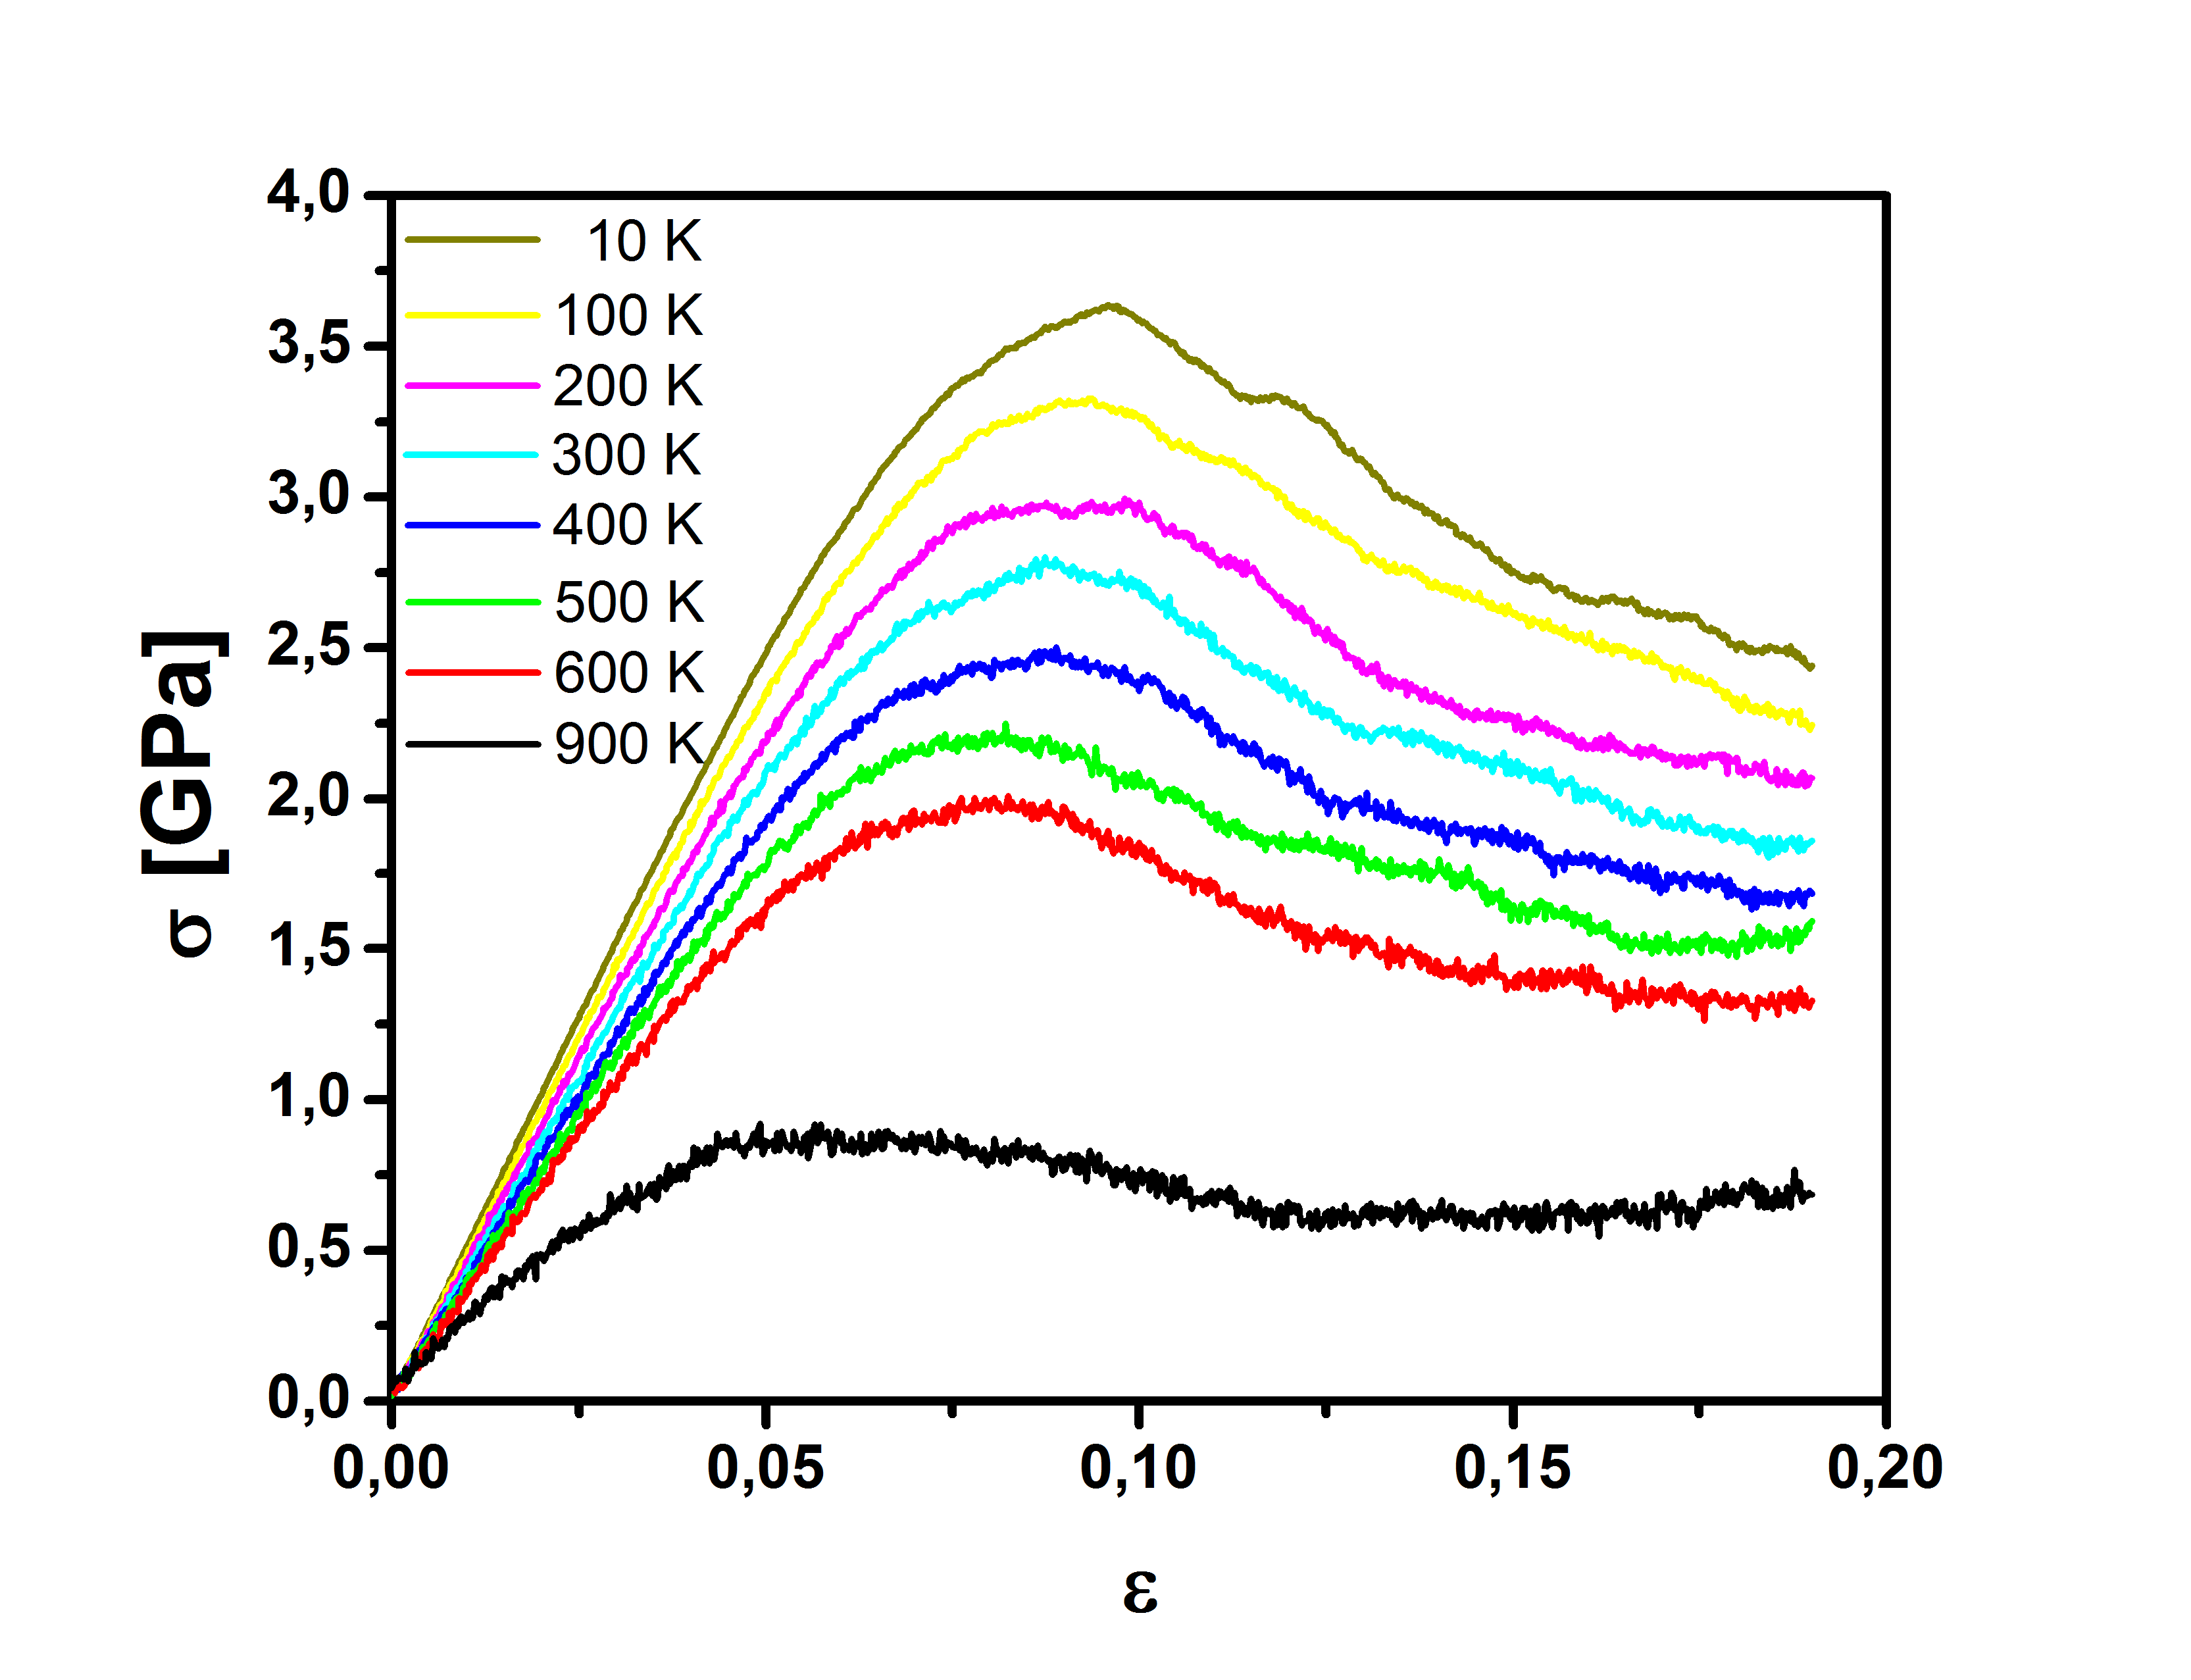
\includegraphics[width=8cm]{Figures/stress_strain_COMP.png}
\caption{Von Mises vs. strain}
\end{figure}

\begin{figure}[H]
\centering
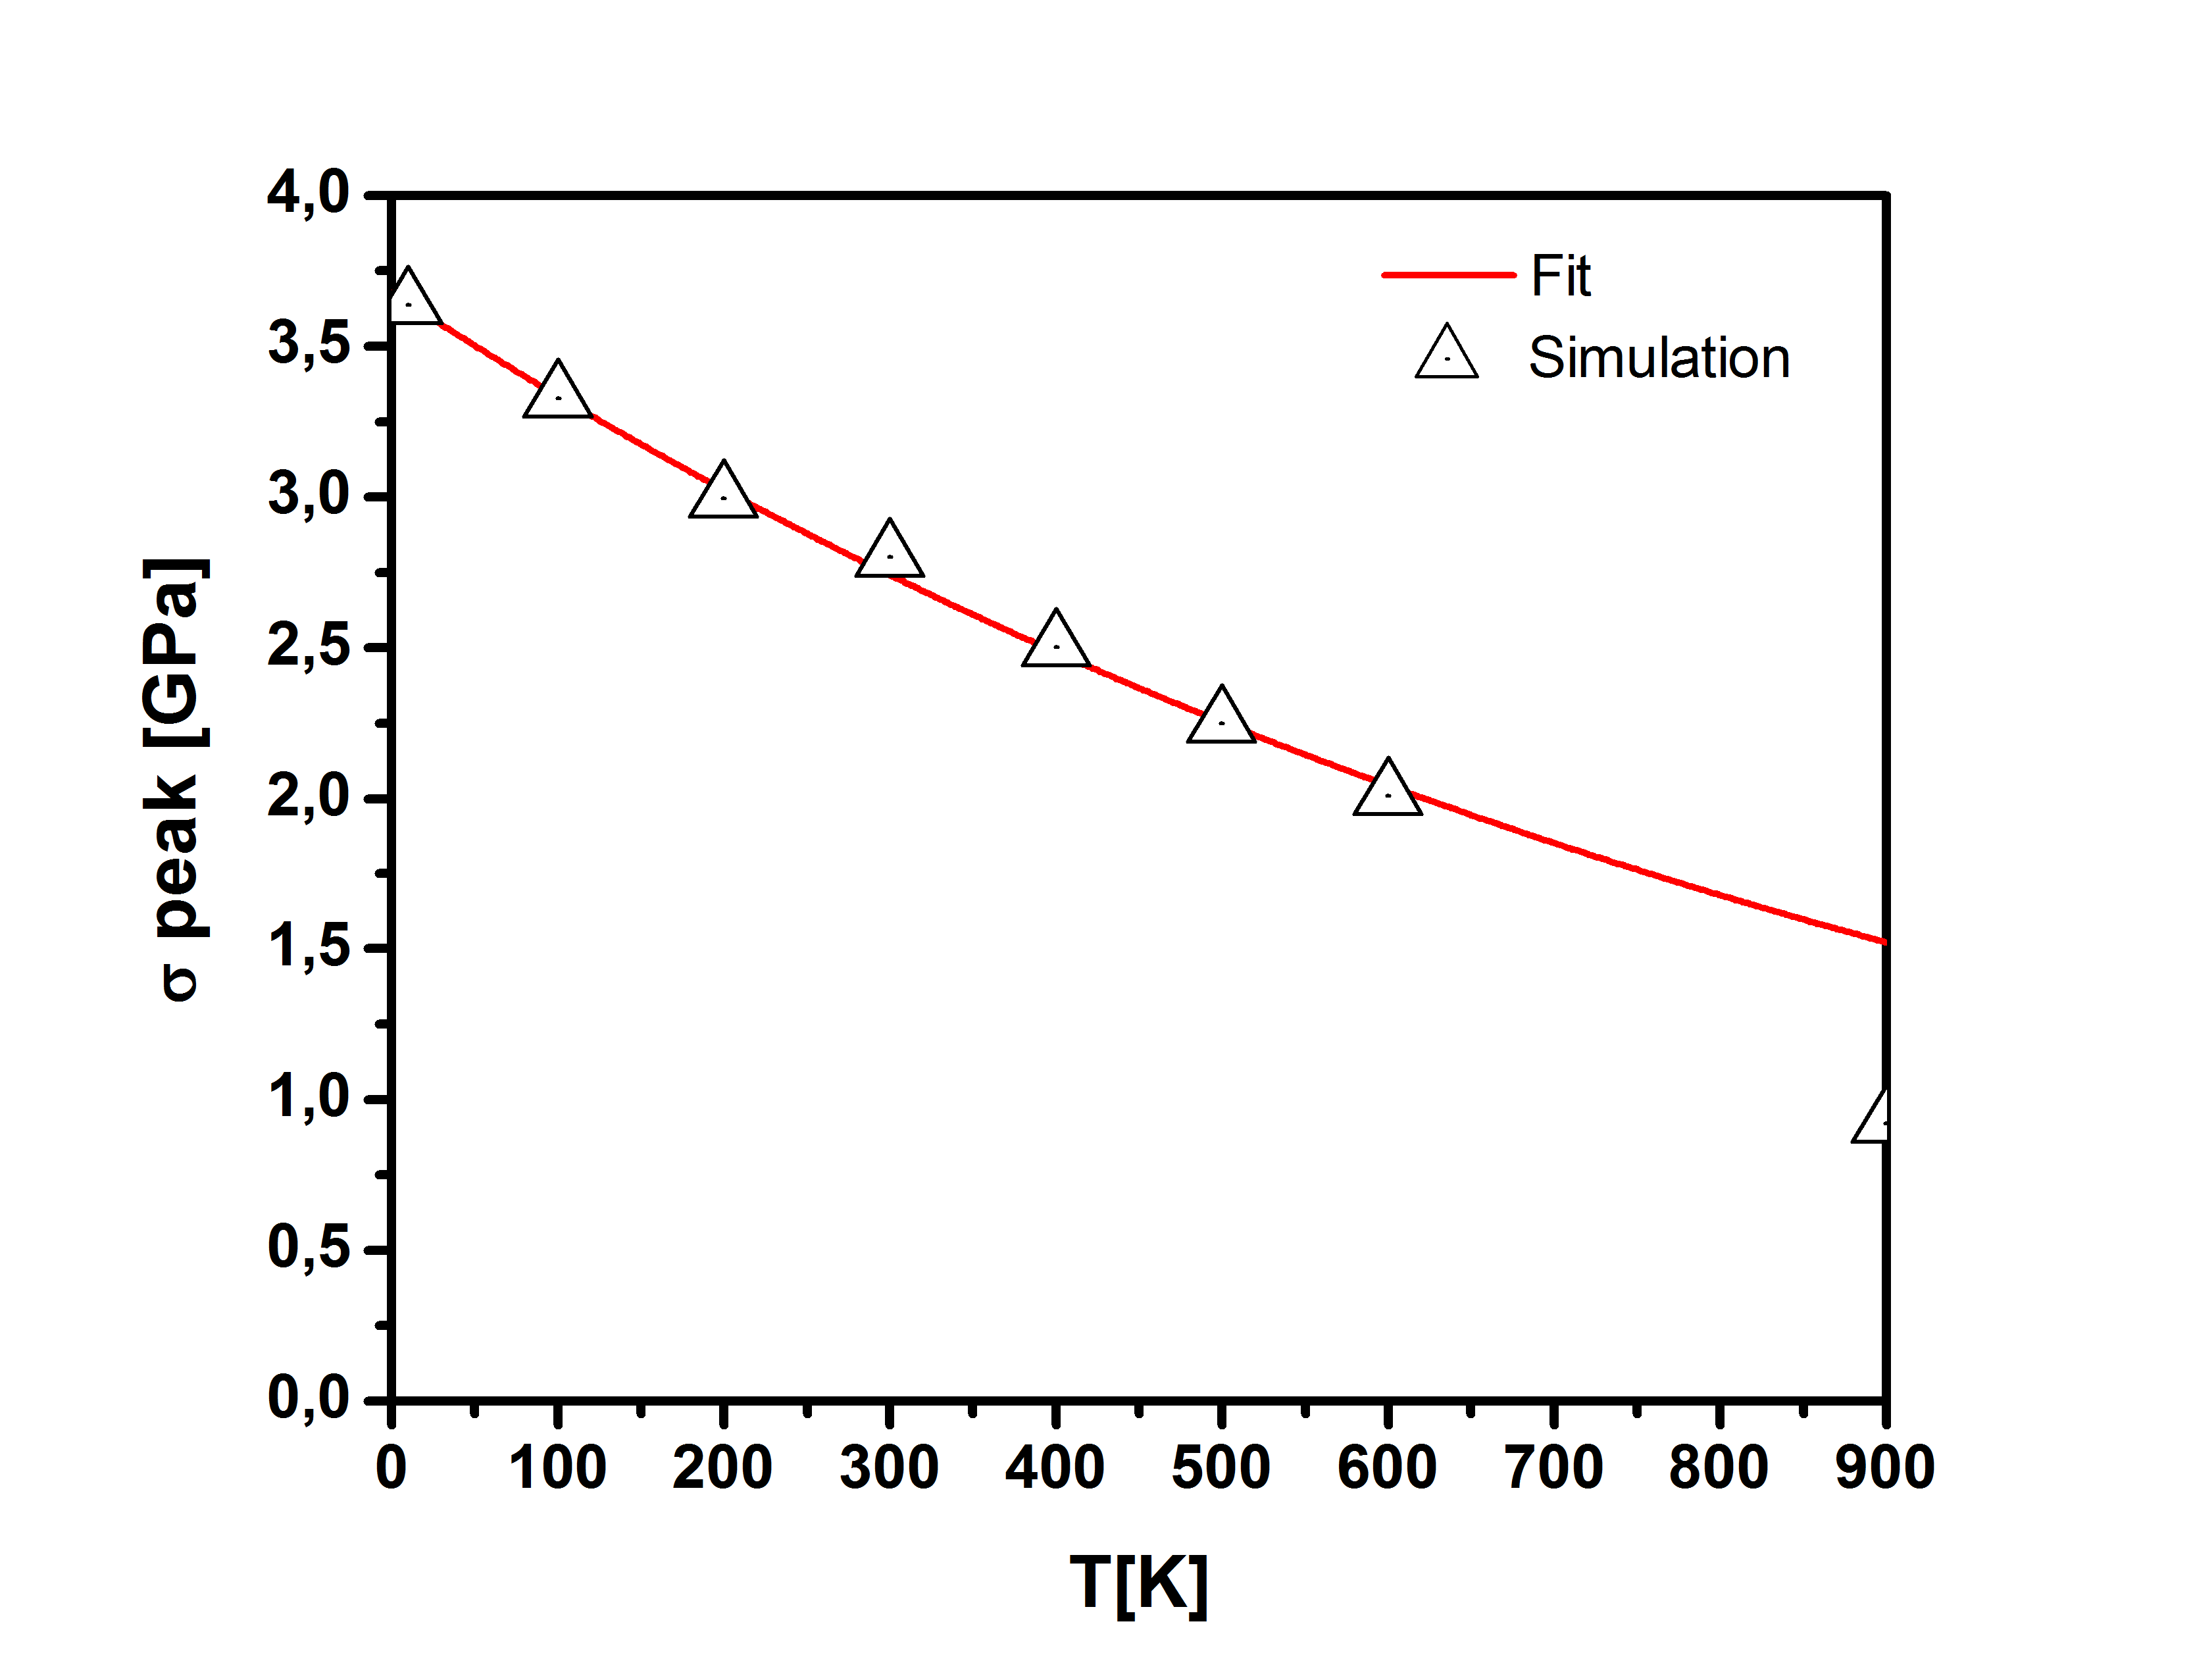
\includegraphics[width=8cm]{Figures/peakstress_T_COMP.png}
\caption{Von Mises maximo vs. Temperatura}
\end{figure}

\begin{figure}[H]
\centering
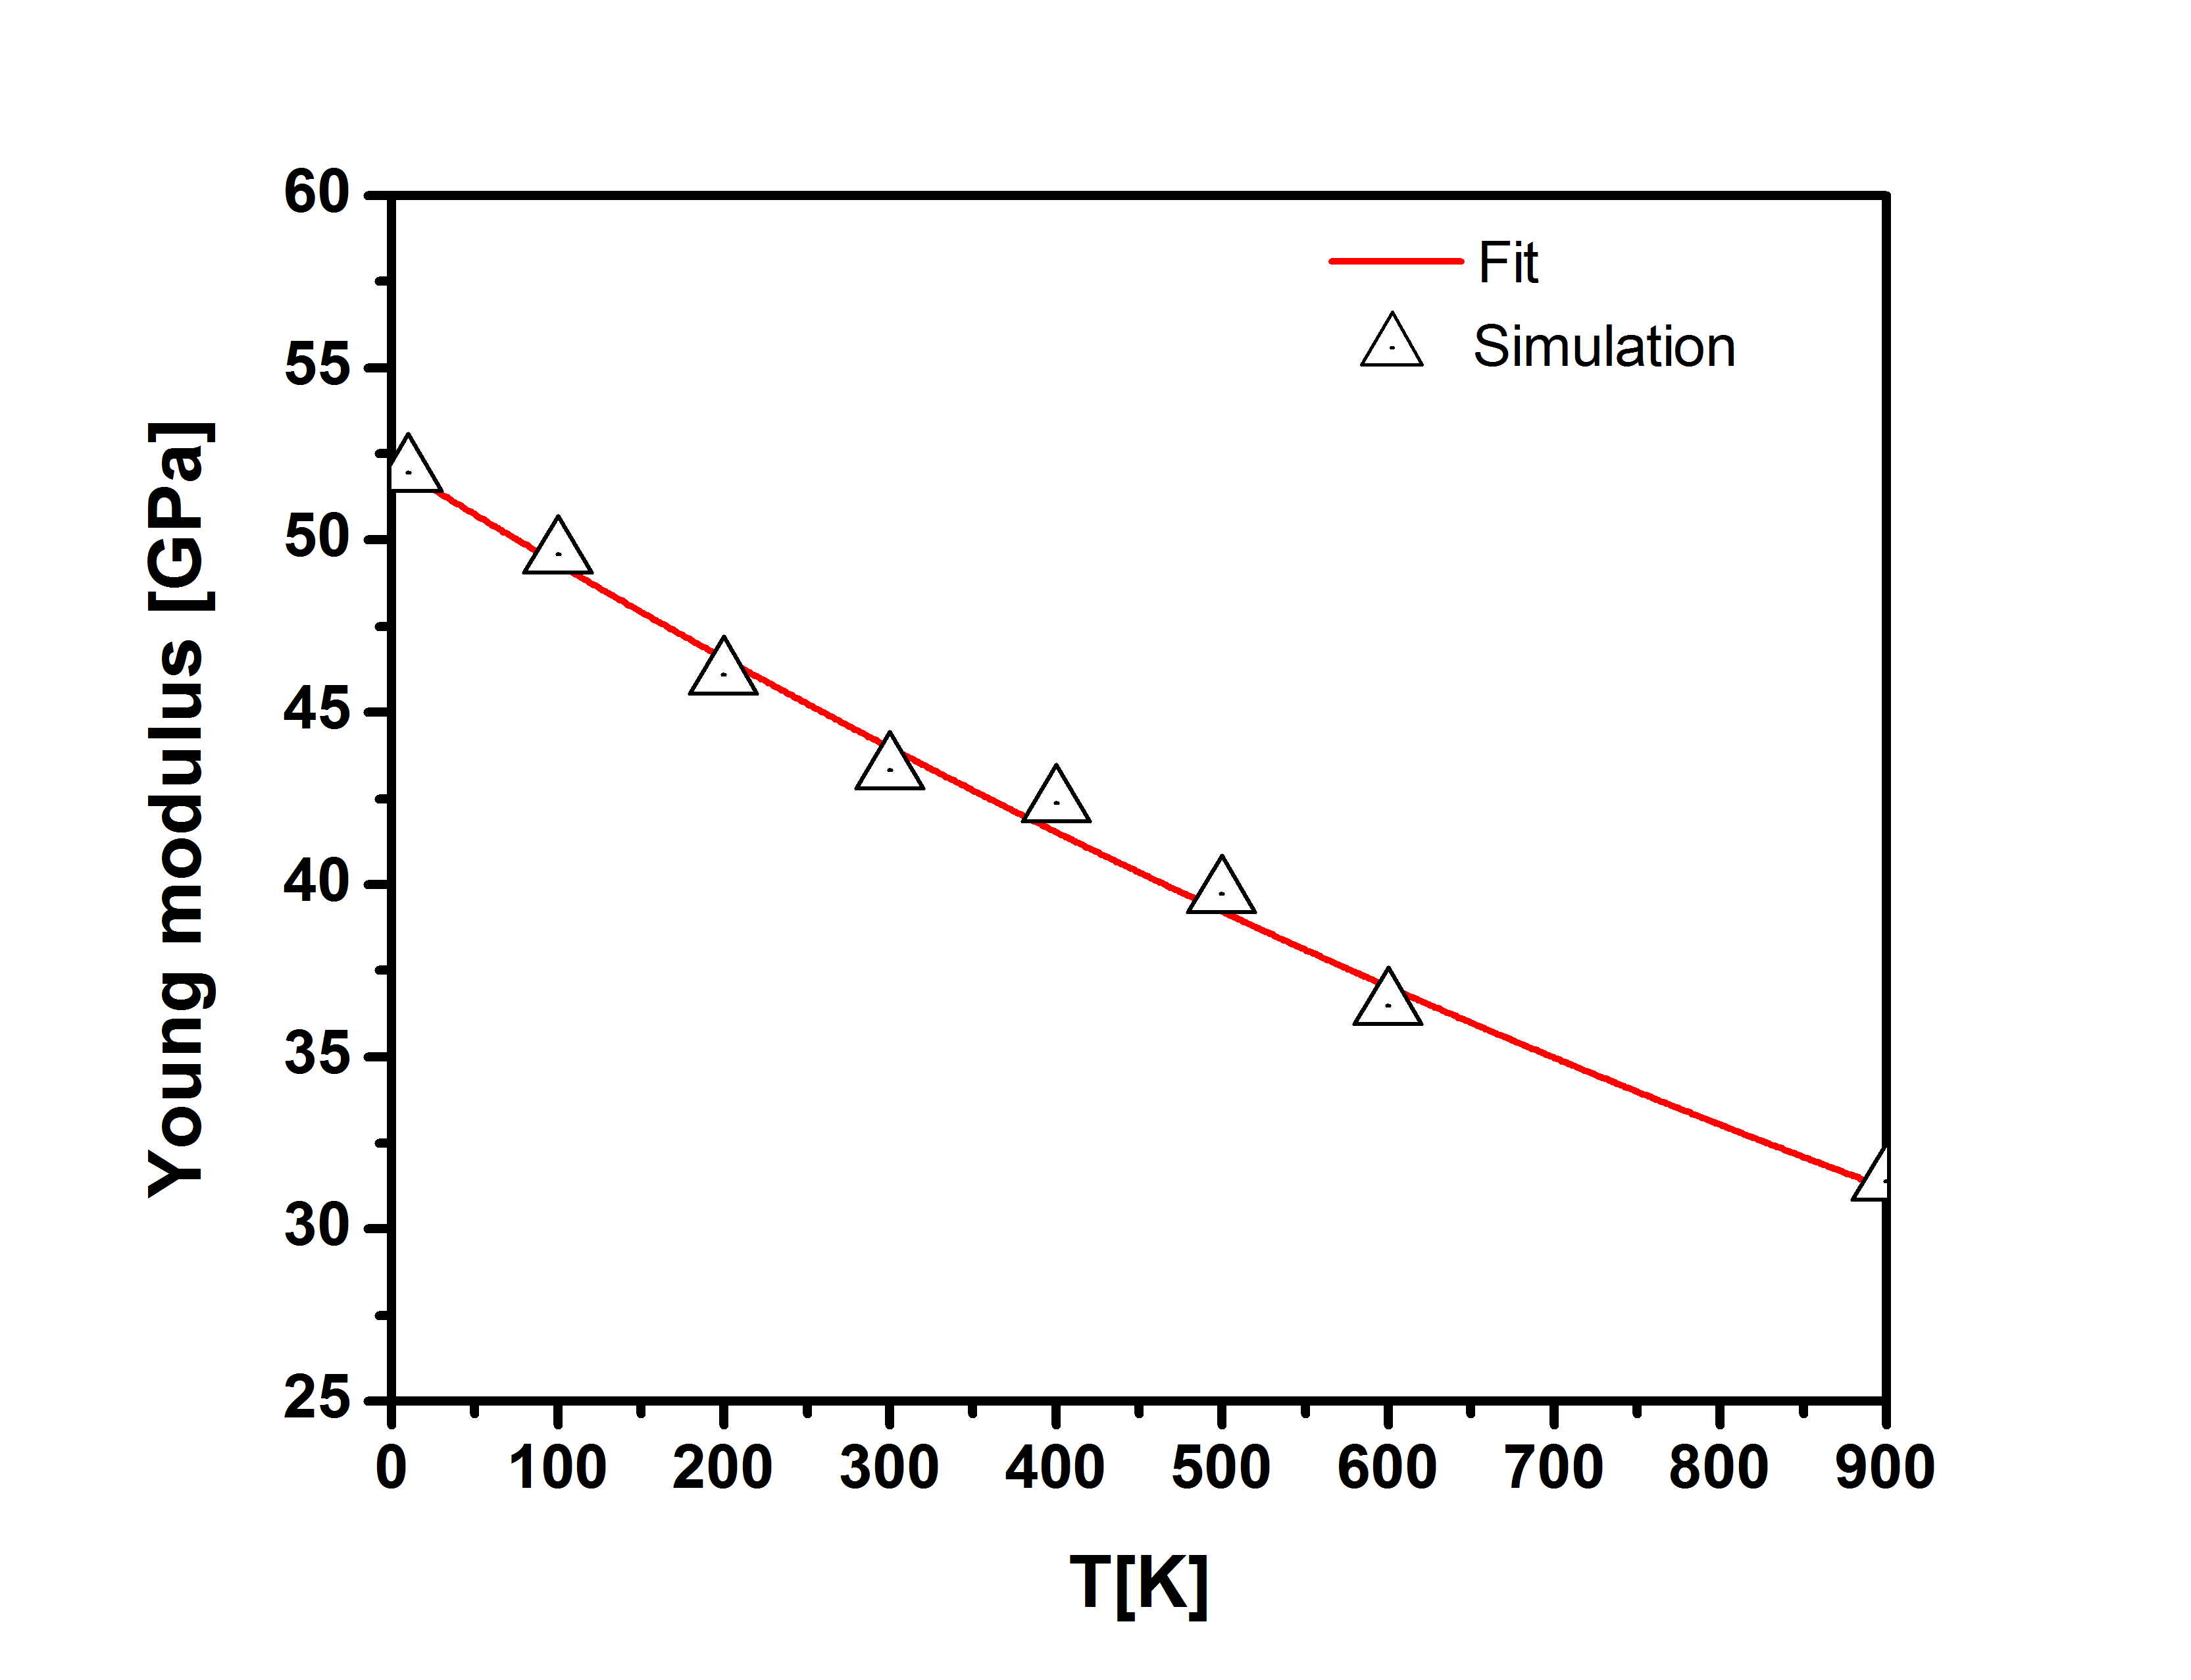
\includegraphics[width=8cm]{Figures/young_T_COMP.png}
\caption{Modulo Young vs. Temperatura}
\end{figure}

\begin{figure}[H]
\centering
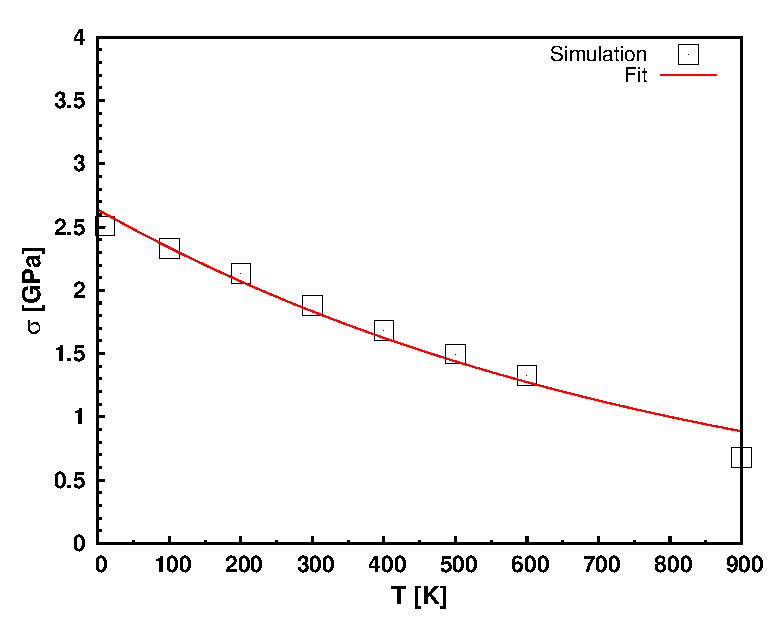
\includegraphics[width=8cm]{Figures/18stress_T_COMP.eps}
\caption{Von Mises a strain 18\% vs. Temperatura}
\end{figure}

\begin{figure}[H]
\centering
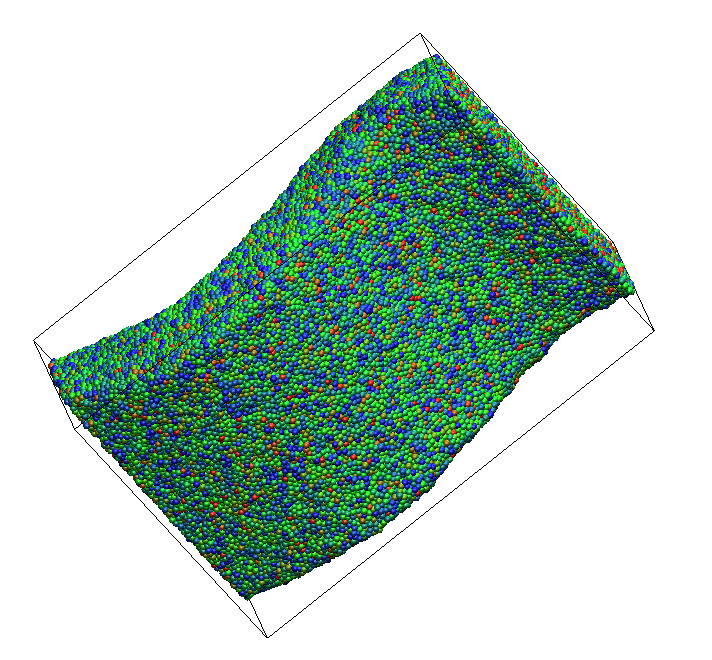
\includegraphics[width=8cm]{Figures/300libresComp.png}
\caption{Muestra a 300K cond. de frontera libres strain 20\%}
\end{figure}

\begin{figure}[H]
\centering
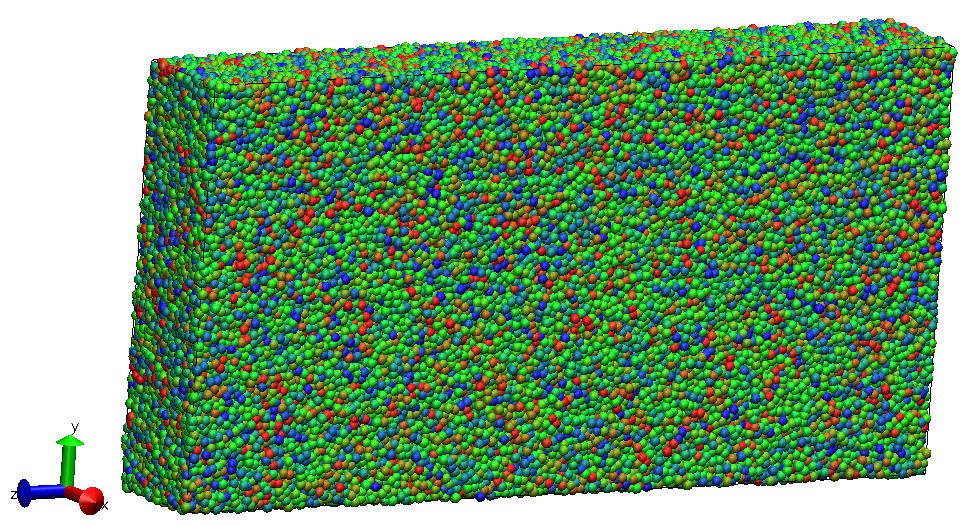
\includegraphics[width=8cm]{Figures/All_300K_6pstrain_sacale100-400_Comp.png}
\caption{Muestra a 300K cond. de frontera periodicas, 6\% strain, escala de colores 100-400 GPa}
\end{figure}

\begin{figure}[H]
\centering
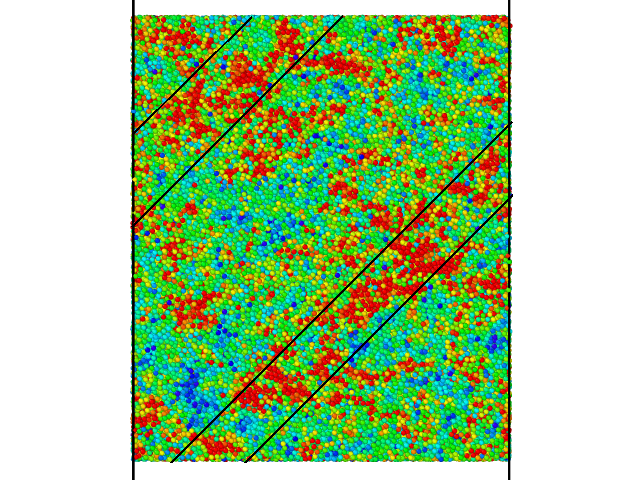
\includegraphics[width=8cm]{Figures/ShearBand.png}
\caption{Shearband a 300K, 14\% strain, escala 0.02 a 0.15 atomic strain}
\end{figure}

\begin{figure}[H]
\centering
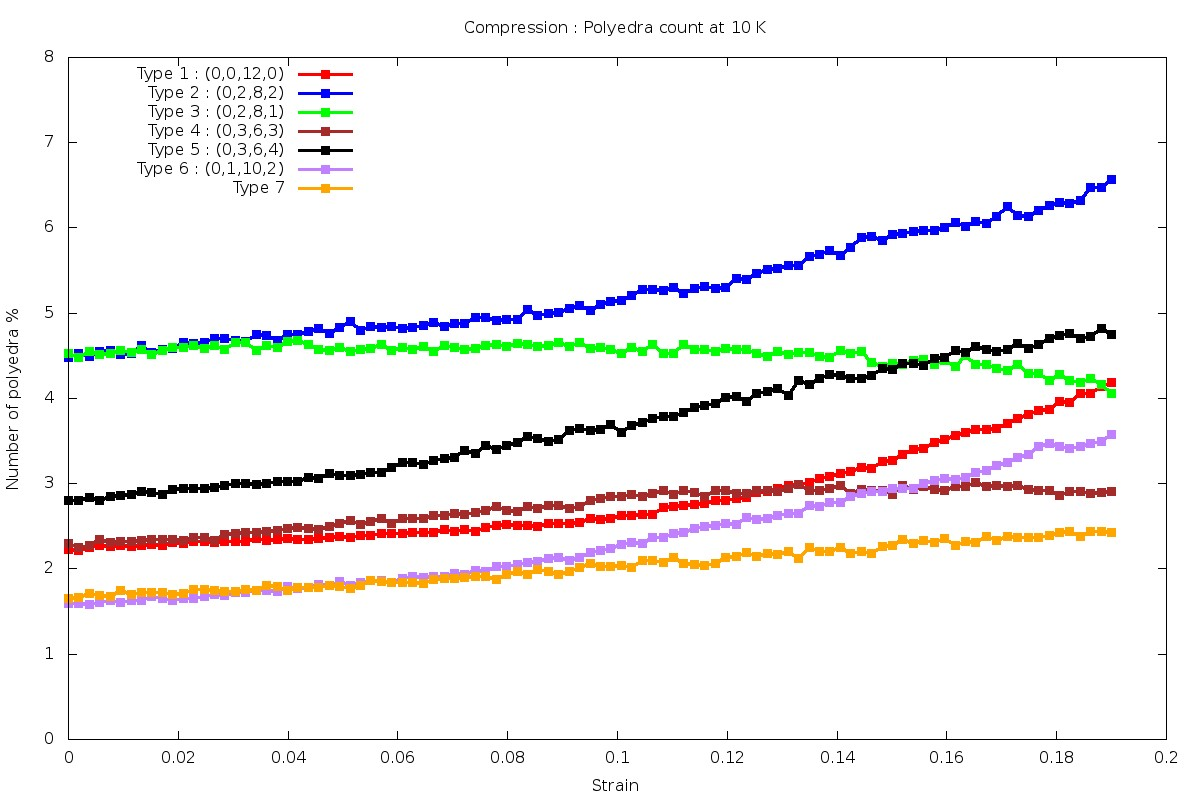
\includegraphics[width=8cm]{Figures/Compr_Polyedra_10K.jpeg}
\caption{Polyedros de voronoi vs. strain para 10K}
\end{figure}

\begin{figure}[H]
\centering
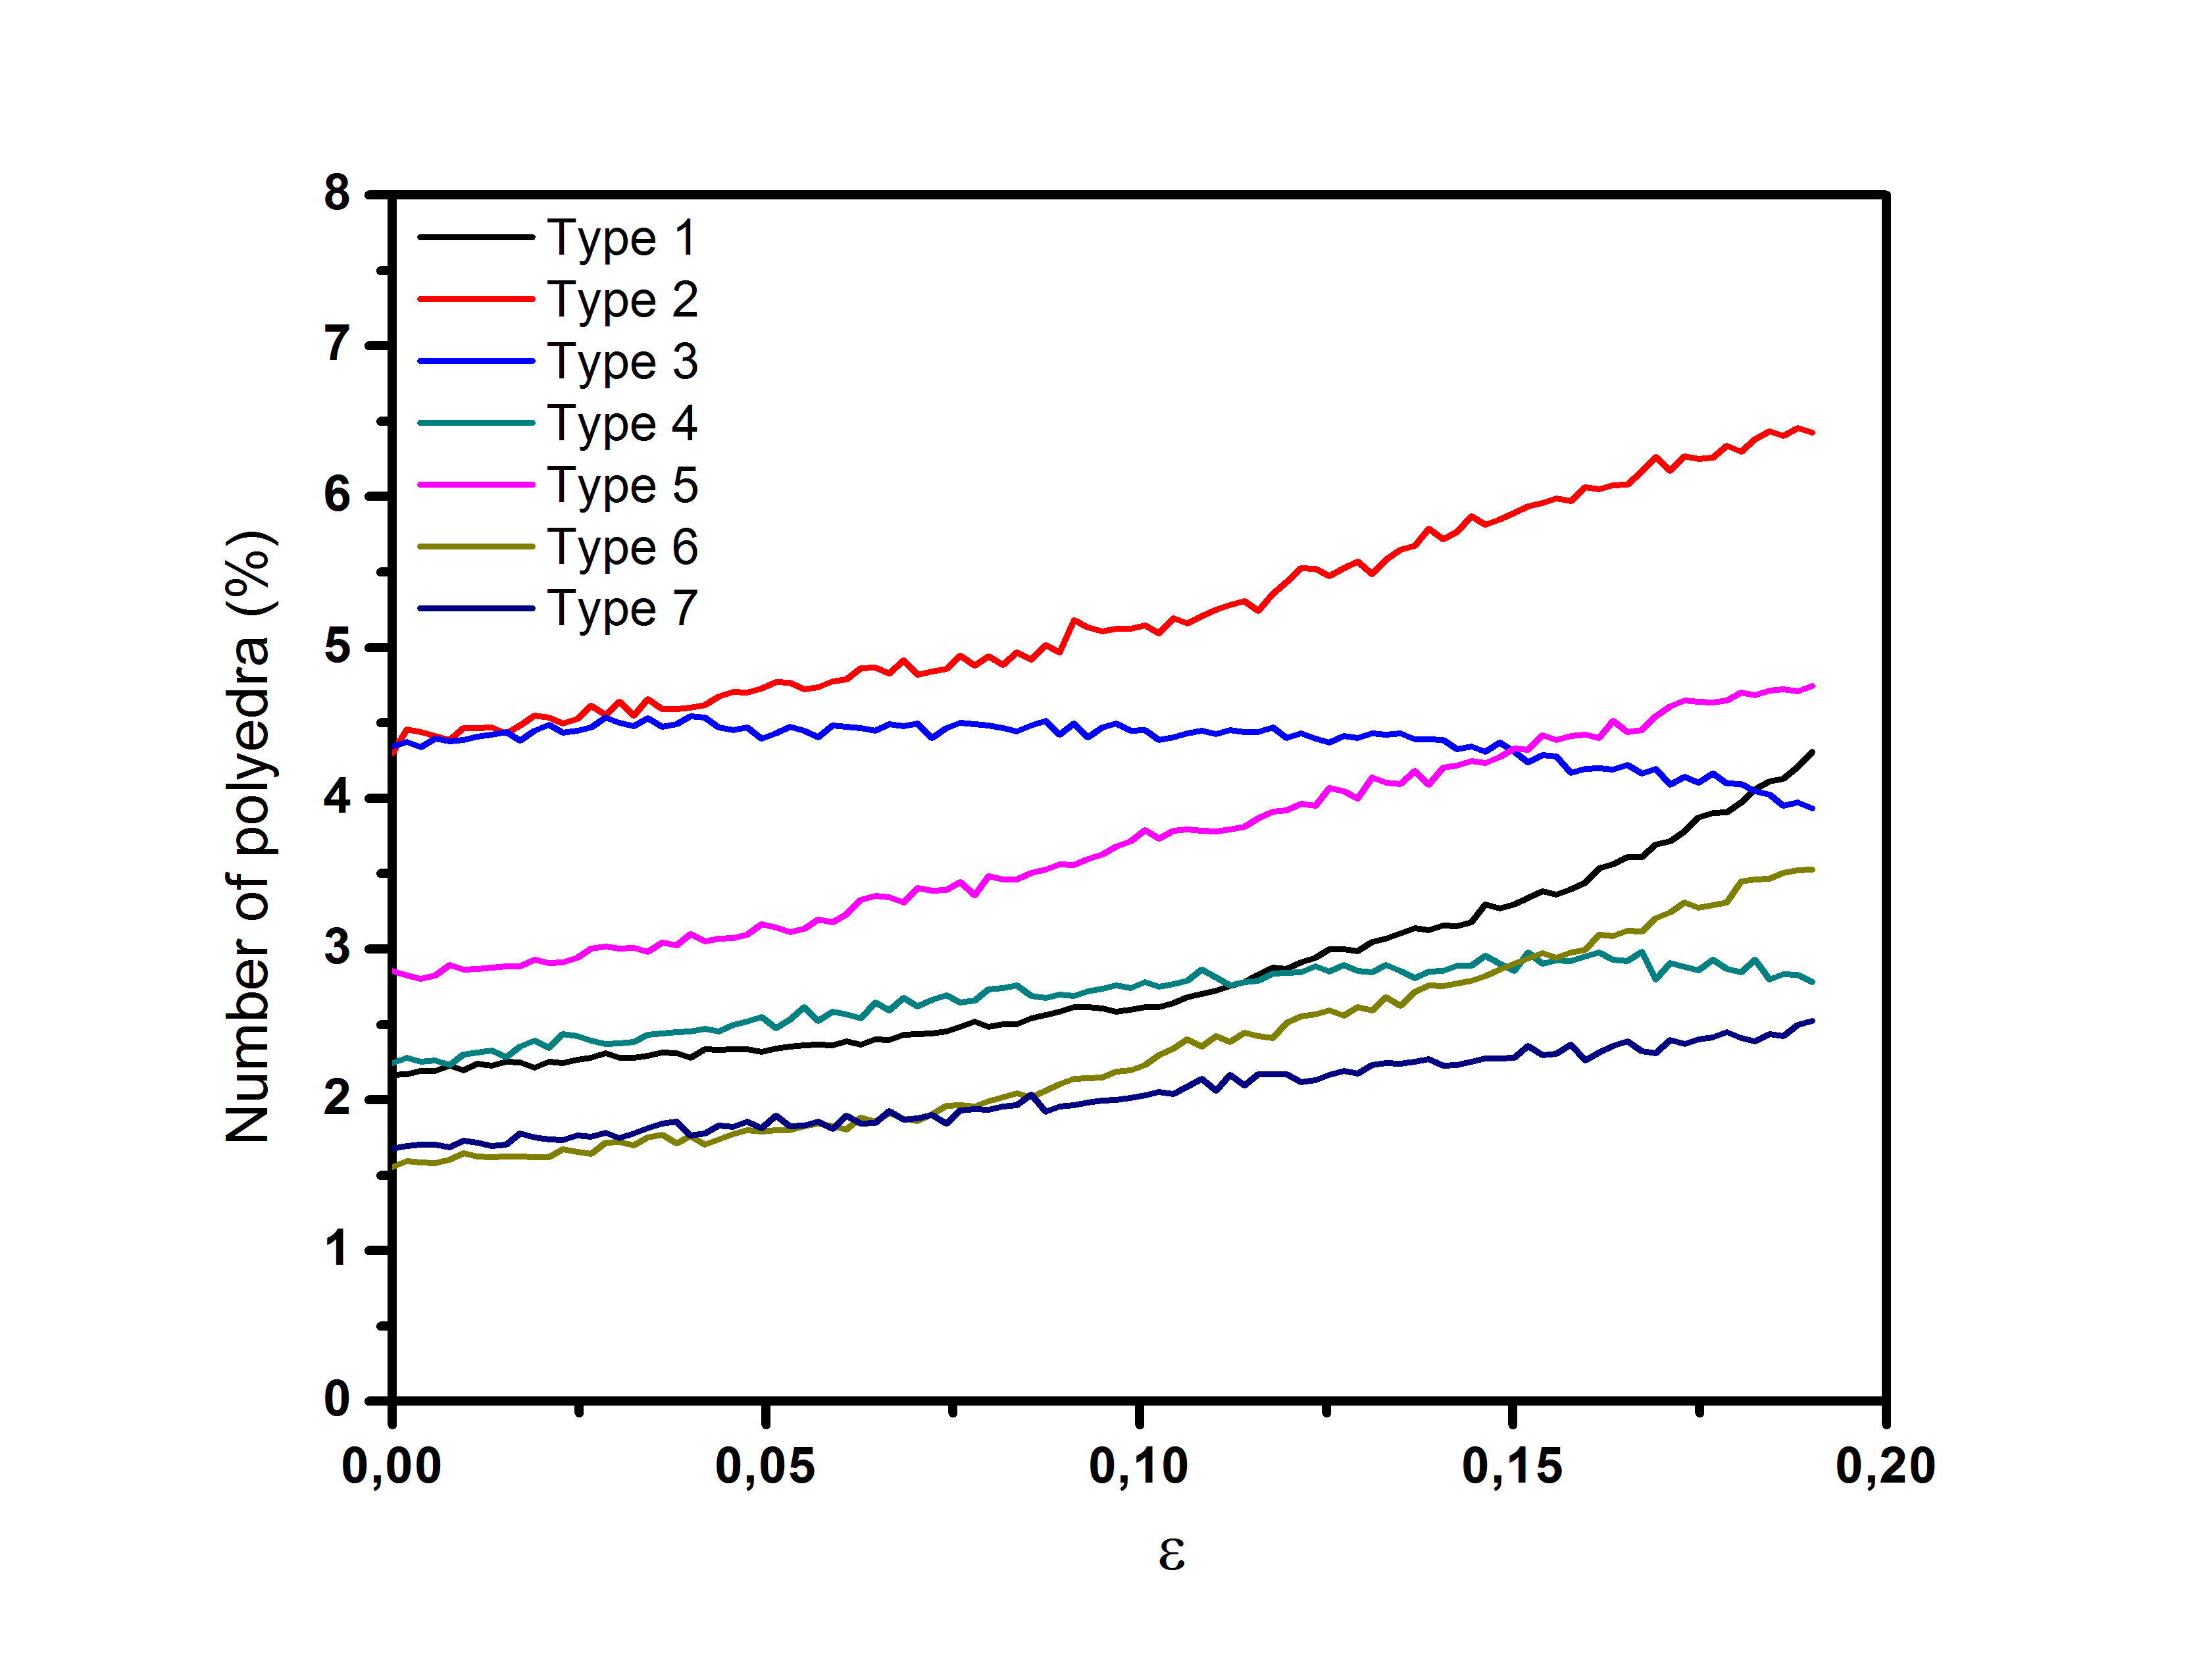
\includegraphics[width=8cm]{Figures/Polyedra_Vs_Strain_100K_COMP.png}
\caption{Num polyedros de voronoi vs. strain, a 100K}
\end{figure}

\begin{figure}[H]
\centering
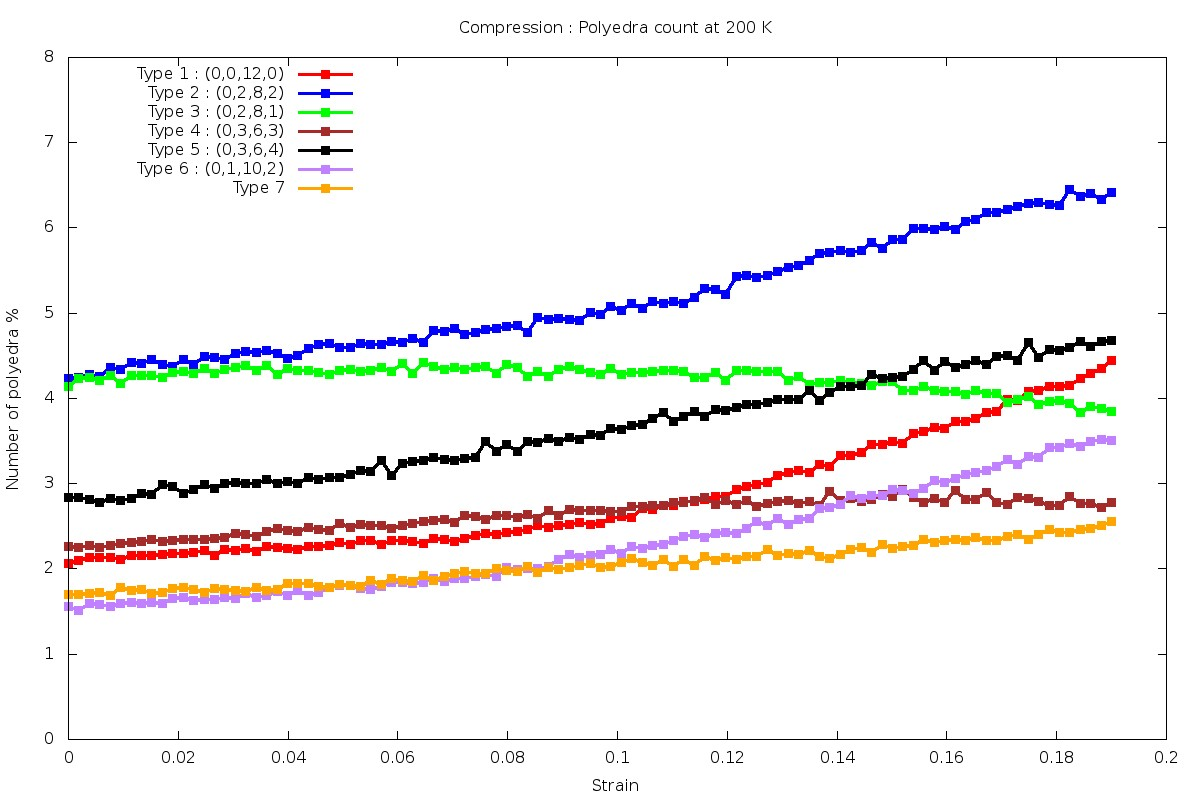
\includegraphics[width=8cm]{Figures/Compr_Polyedra_200K.jpeg}
\caption{Polyedros de voronoi vs. strain para 200K}
\end{figure}

\begin{figure}[H]
\centering
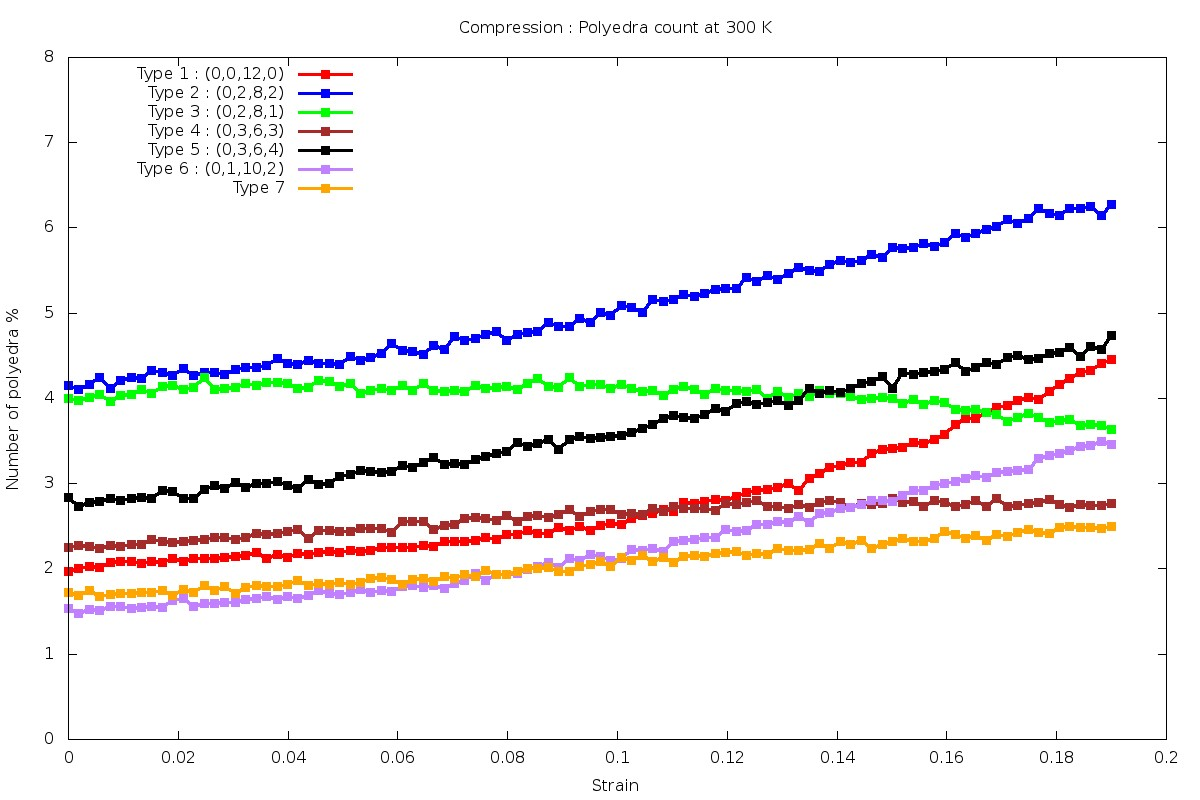
\includegraphics[width=8cm]{Figures/Compr_Polyedra_300K.jpeg}
\caption{Polyedros de voronoi vs. strain para 300K}
\end{figure}

\begin{figure}[H]
\centering
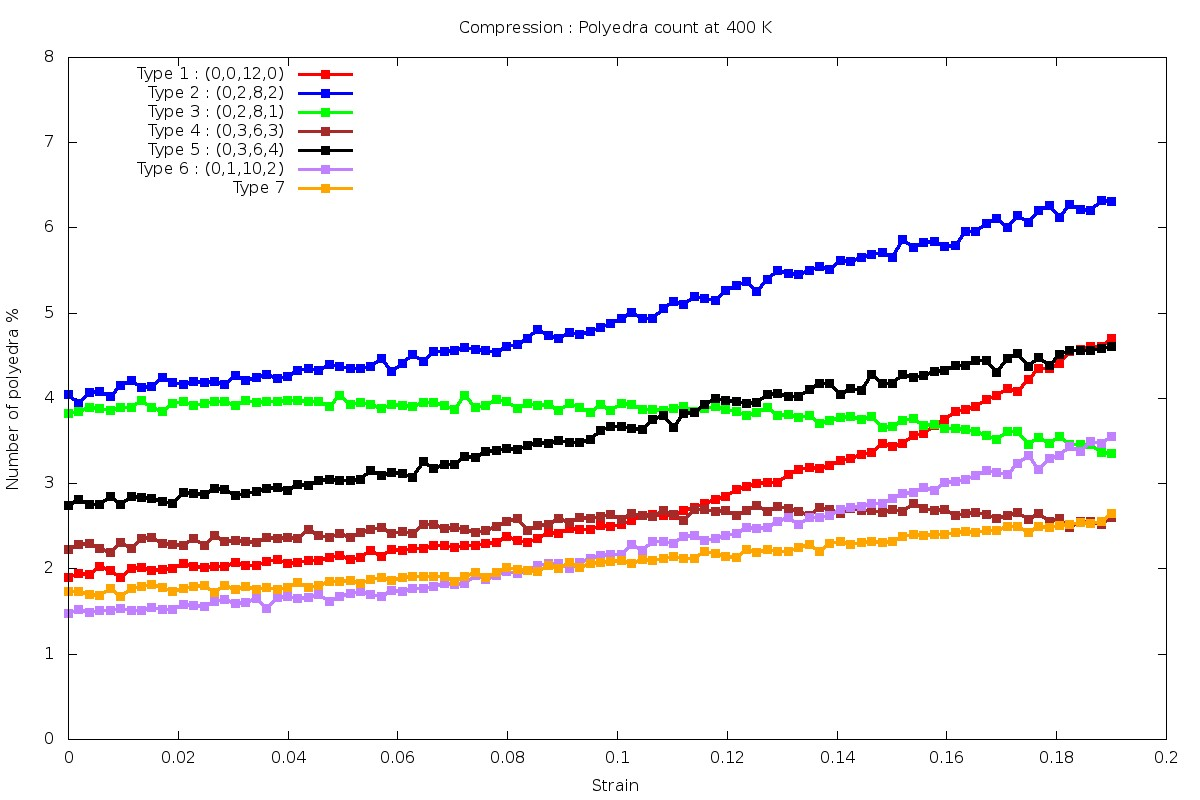
\includegraphics[width=8cm]{Figures/Compr_Polyedra_400K.jpeg}
\caption{Polyedros de voronoi vs. strain para 400K}
\end{figure}

\begin{figure}[H]
\centering
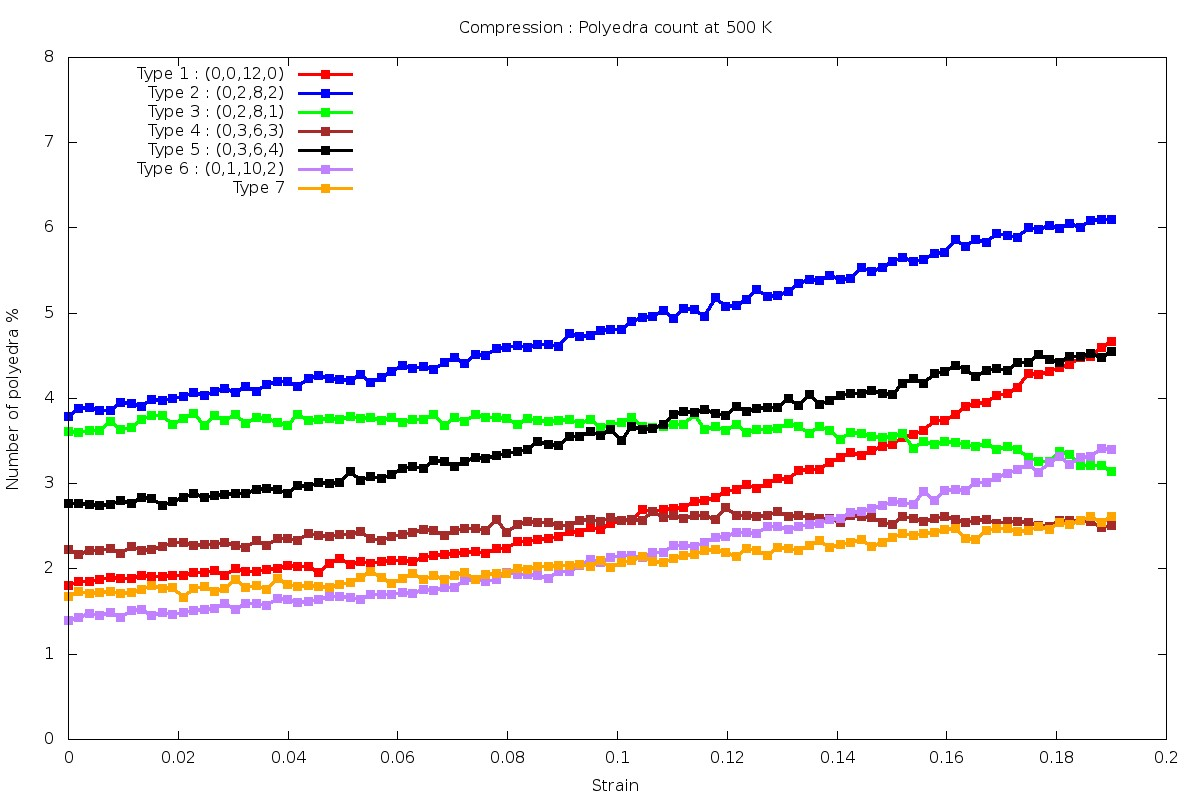
\includegraphics[width=8cm]{Figures/Compr_Polyedra_500K.jpeg}
\caption{Polyedros de voronoi vs. strain para 500K}
\end{figure}

\begin{figure}[H]
\centering
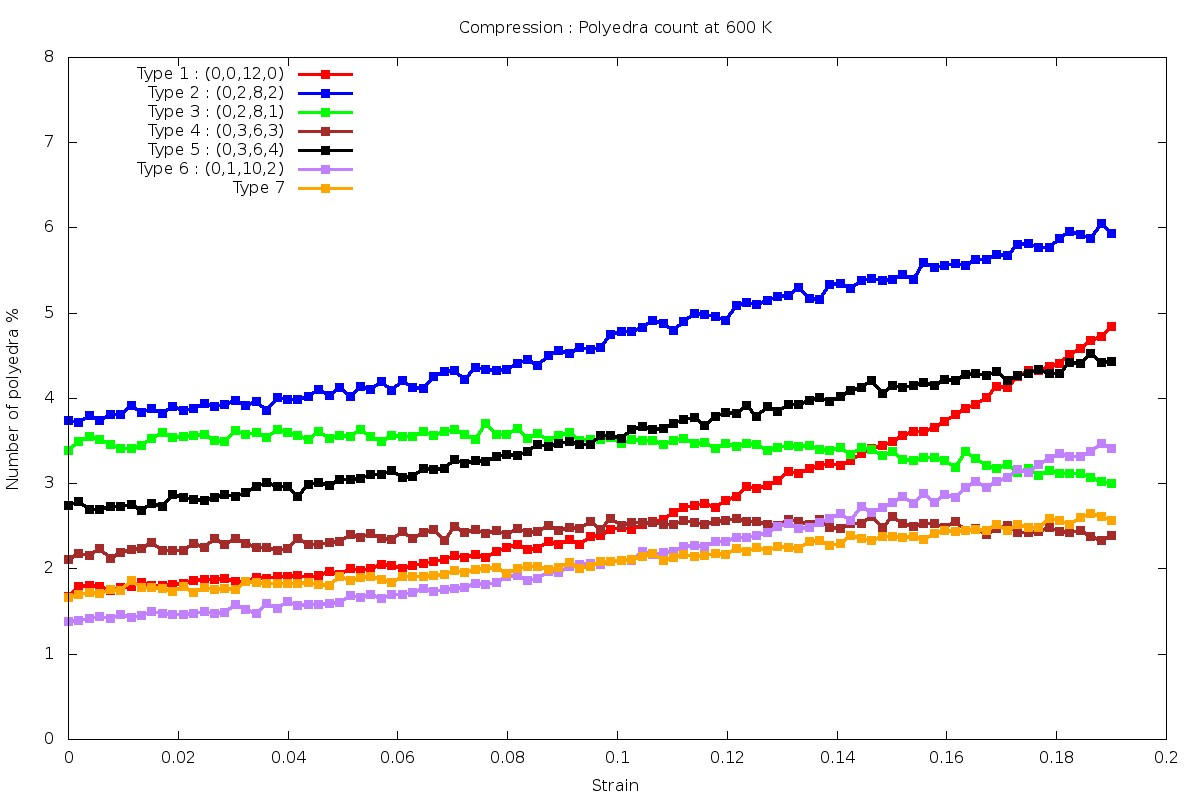
\includegraphics[width=8cm]{Figures/Compr_Polyedra_600K.jpeg}
\caption{Polyedros de voronoi vs. strain para 600K}
\end{figure}

\begin{figure}[H]
\centering
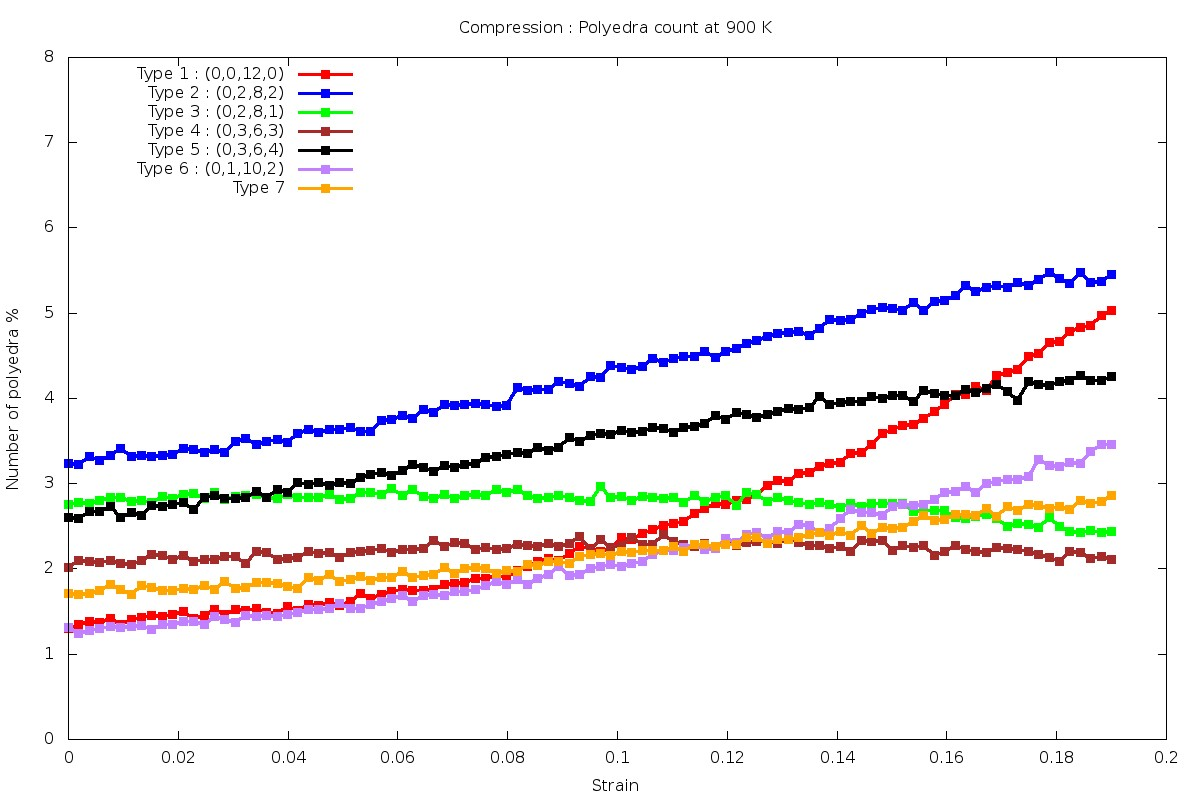
\includegraphics[width=8cm]{Figures/Compr_Polyedra_900K.jpeg}
\caption{Polyedros de voronoi vs. strain para 900K}
\end{figure}

\begin{figure}[H]
\centering
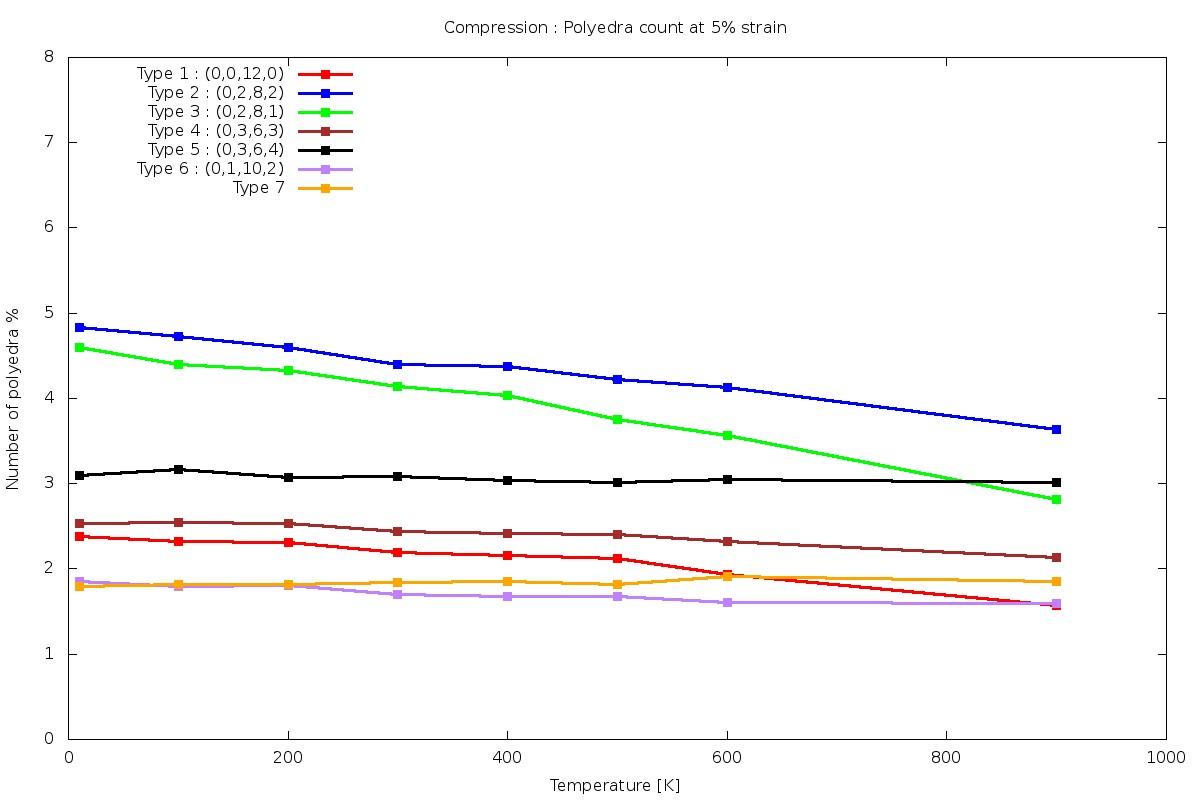
\includegraphics[width=8cm]{Figures/Compr_Voro_Temp_5.jpeg}
\caption{Num polyedros de voronoi vs. temperatura, a strain 5\%}
\end{figure}

\begin{figure}[H]
\centering
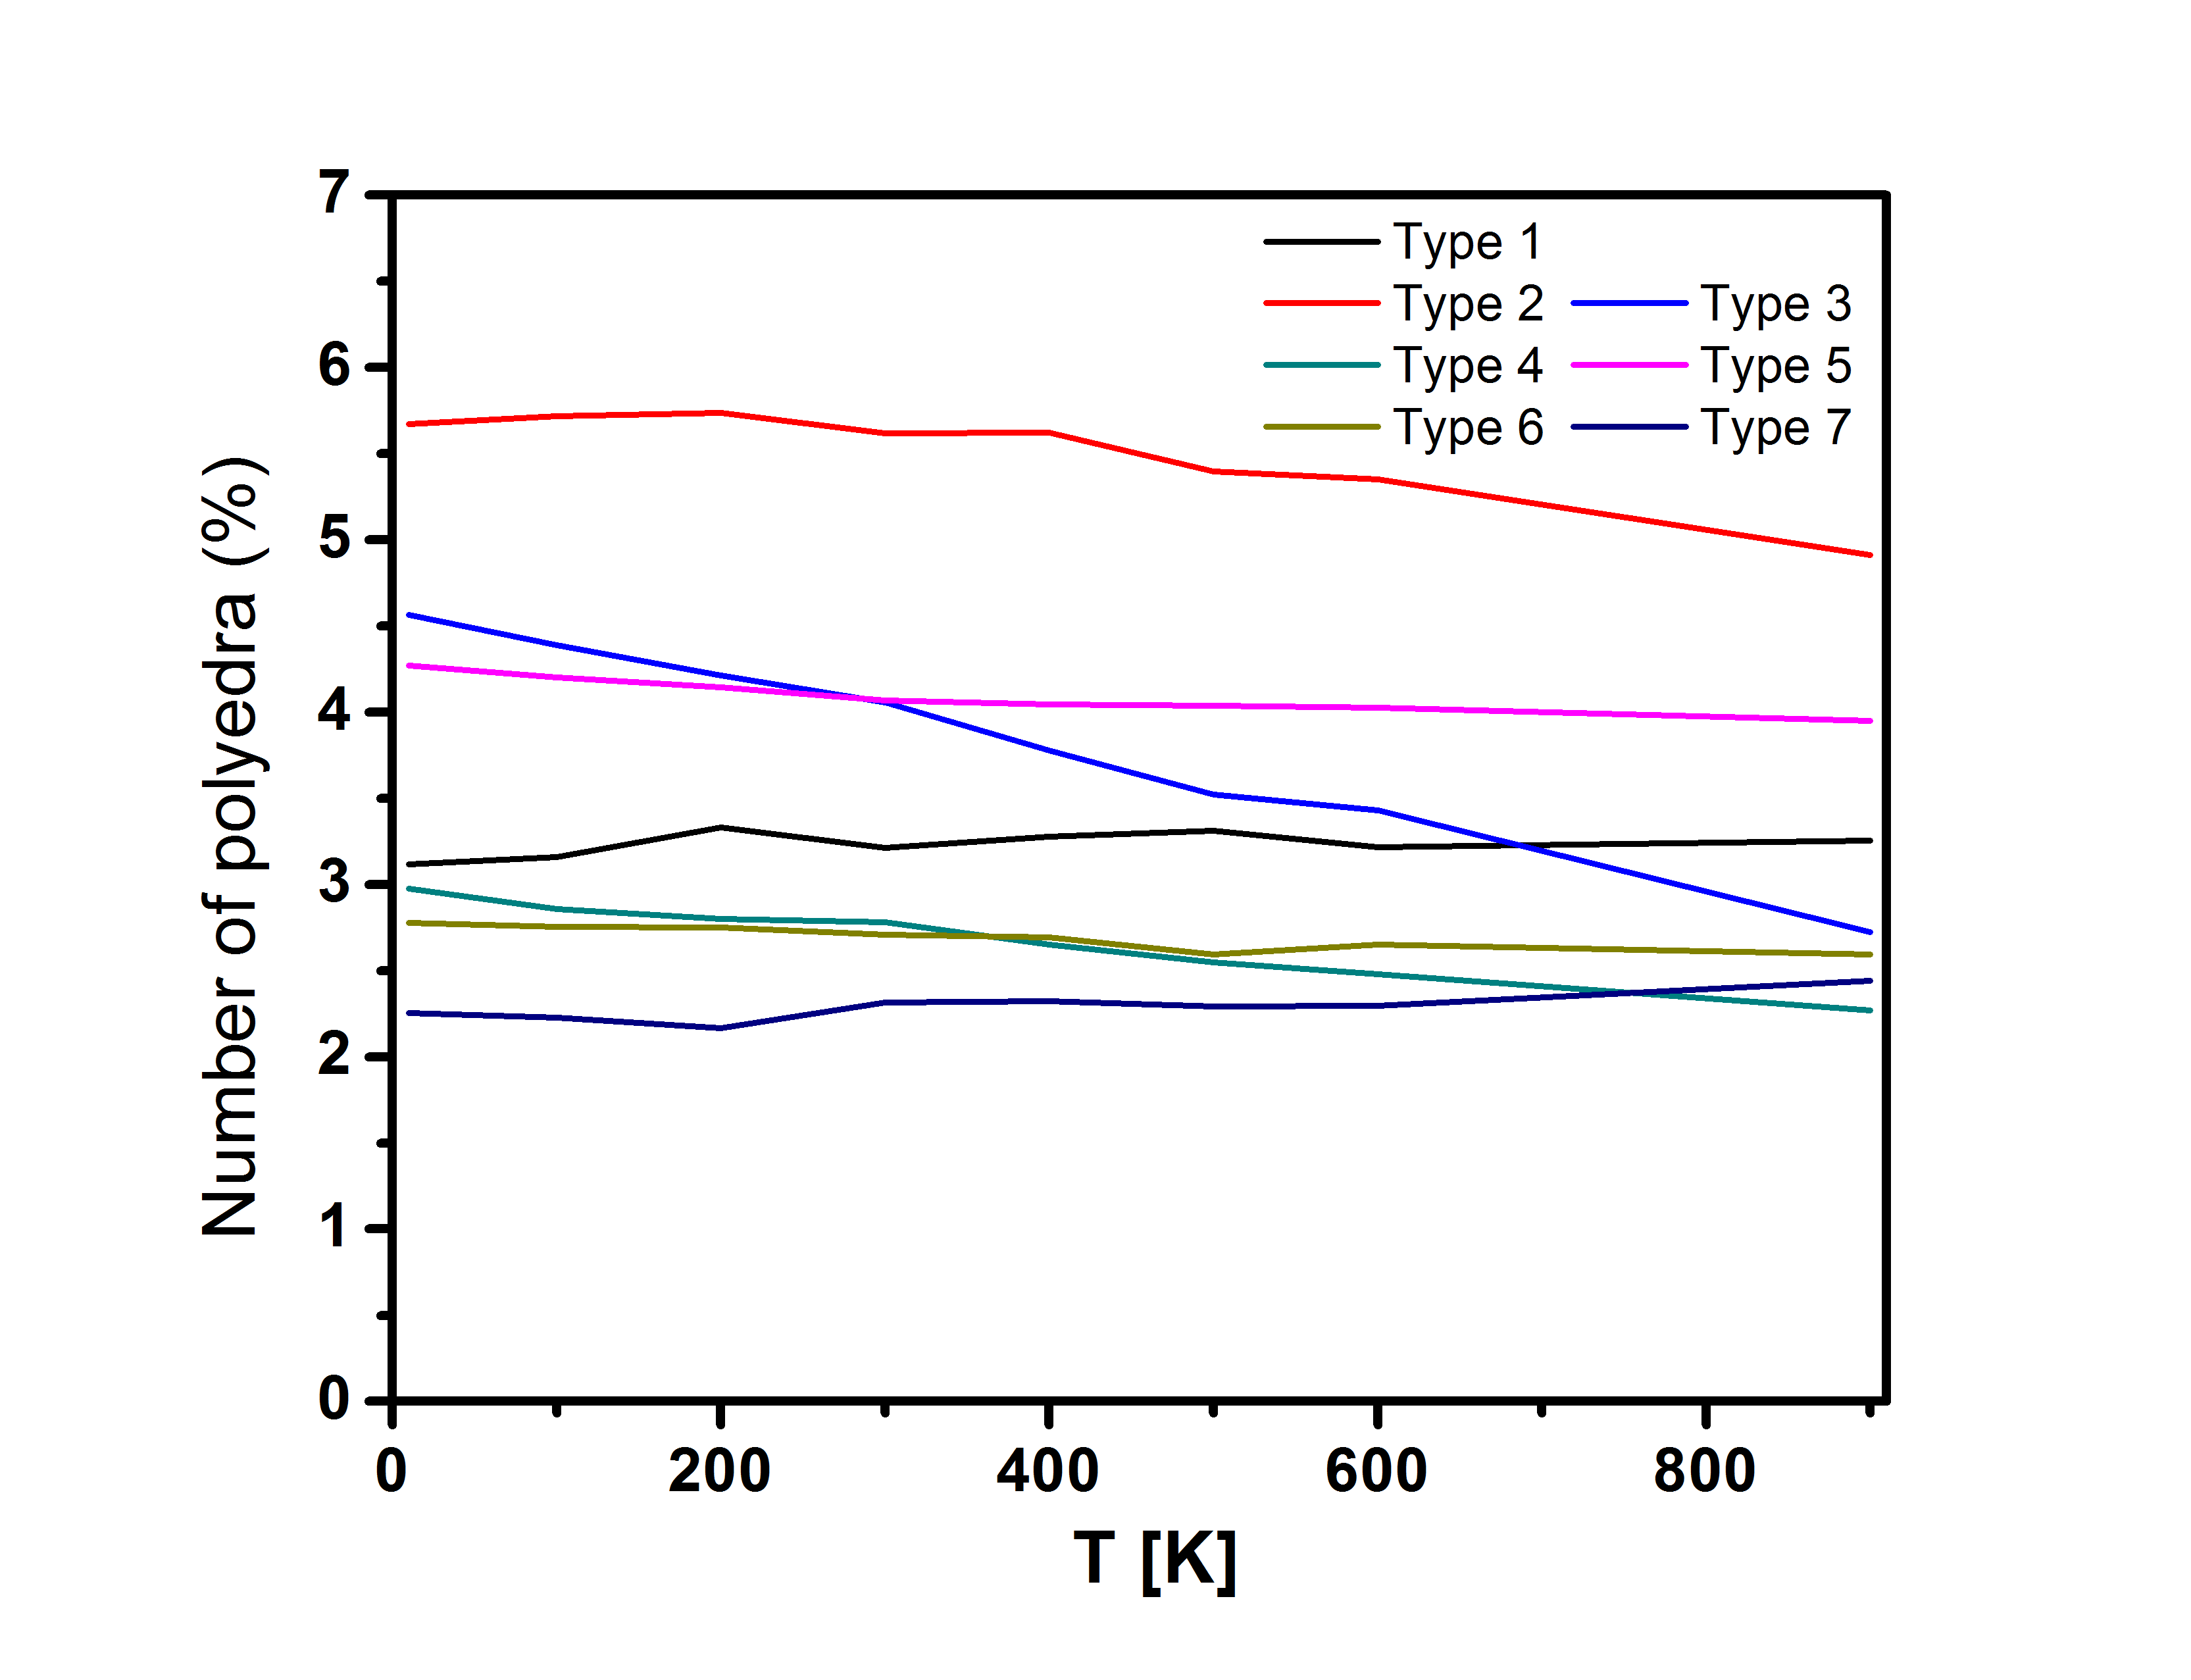
\includegraphics[width=8cm]{Figures/poly_T_14strain_COMP.png}
\caption{Num polyedros de voronoi vs. temperatura, a strain 14\%}
\end{figure}

\begin{figure}[H]
\centering
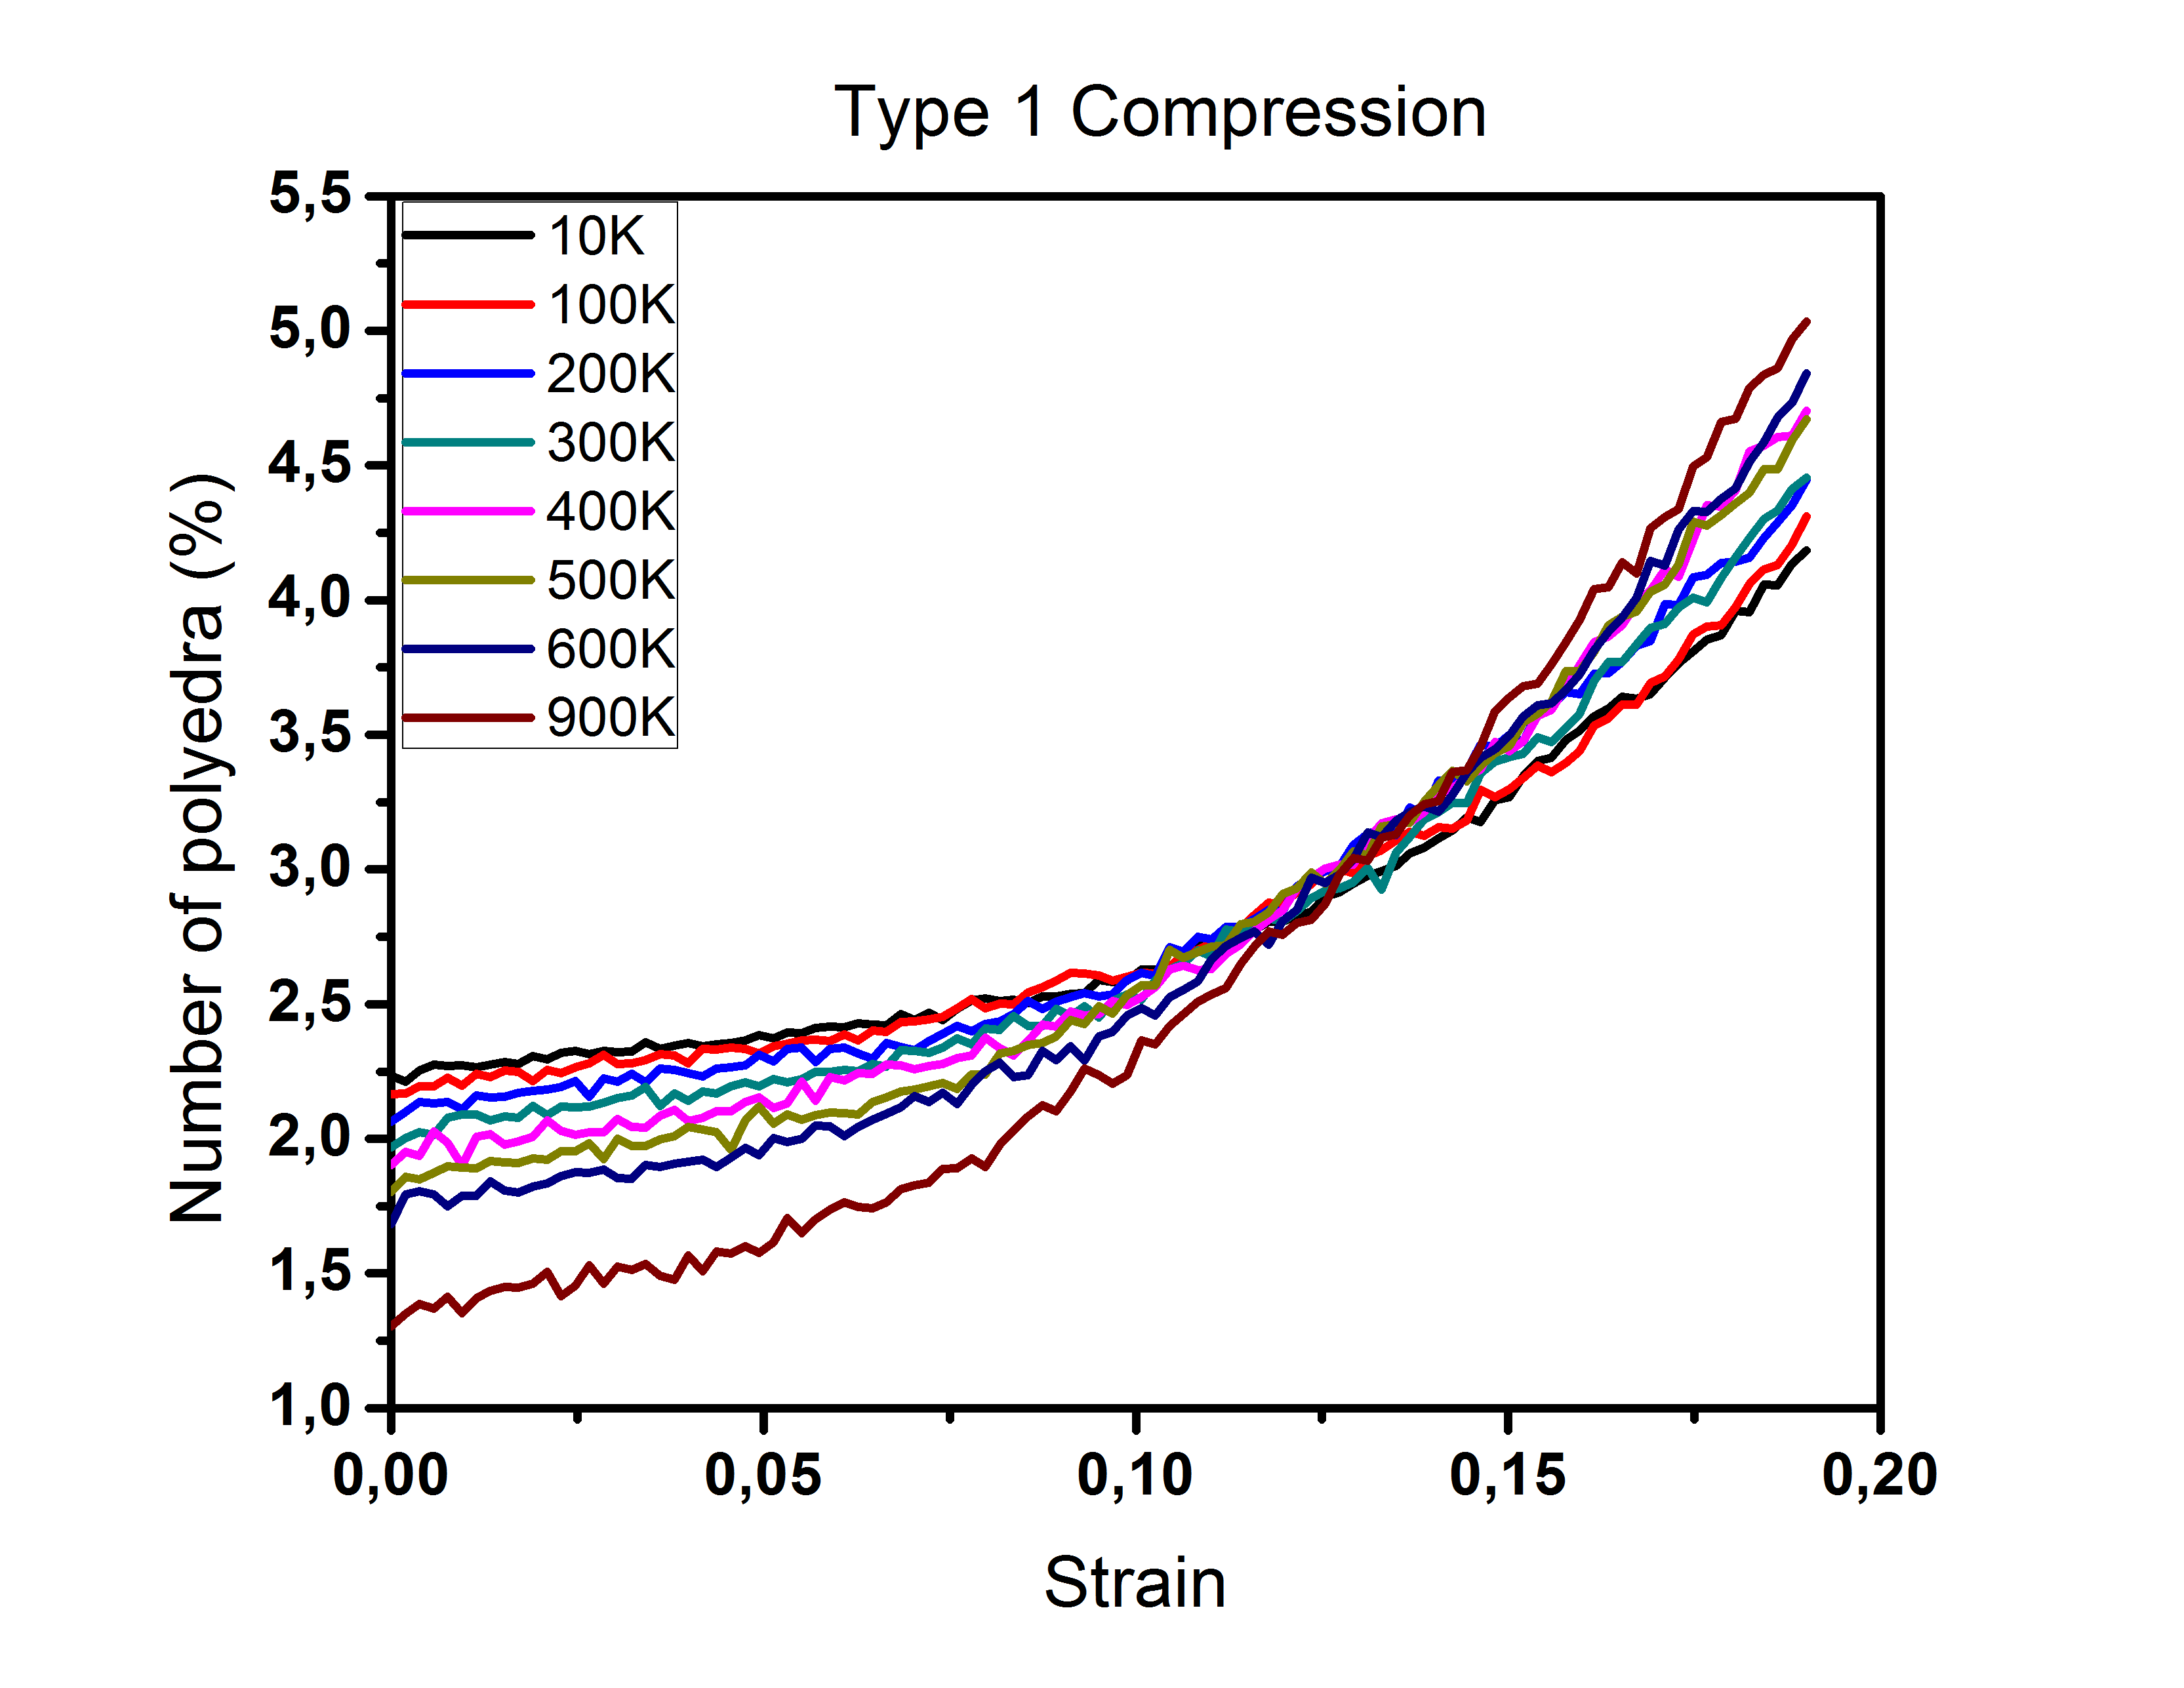
\includegraphics[width=8cm]{Figures/type1_COMP.png}
\caption{polyedros de voronoi tipo 1 vs. strain}
\end{figure}

\begin{figure}[H]
\centering
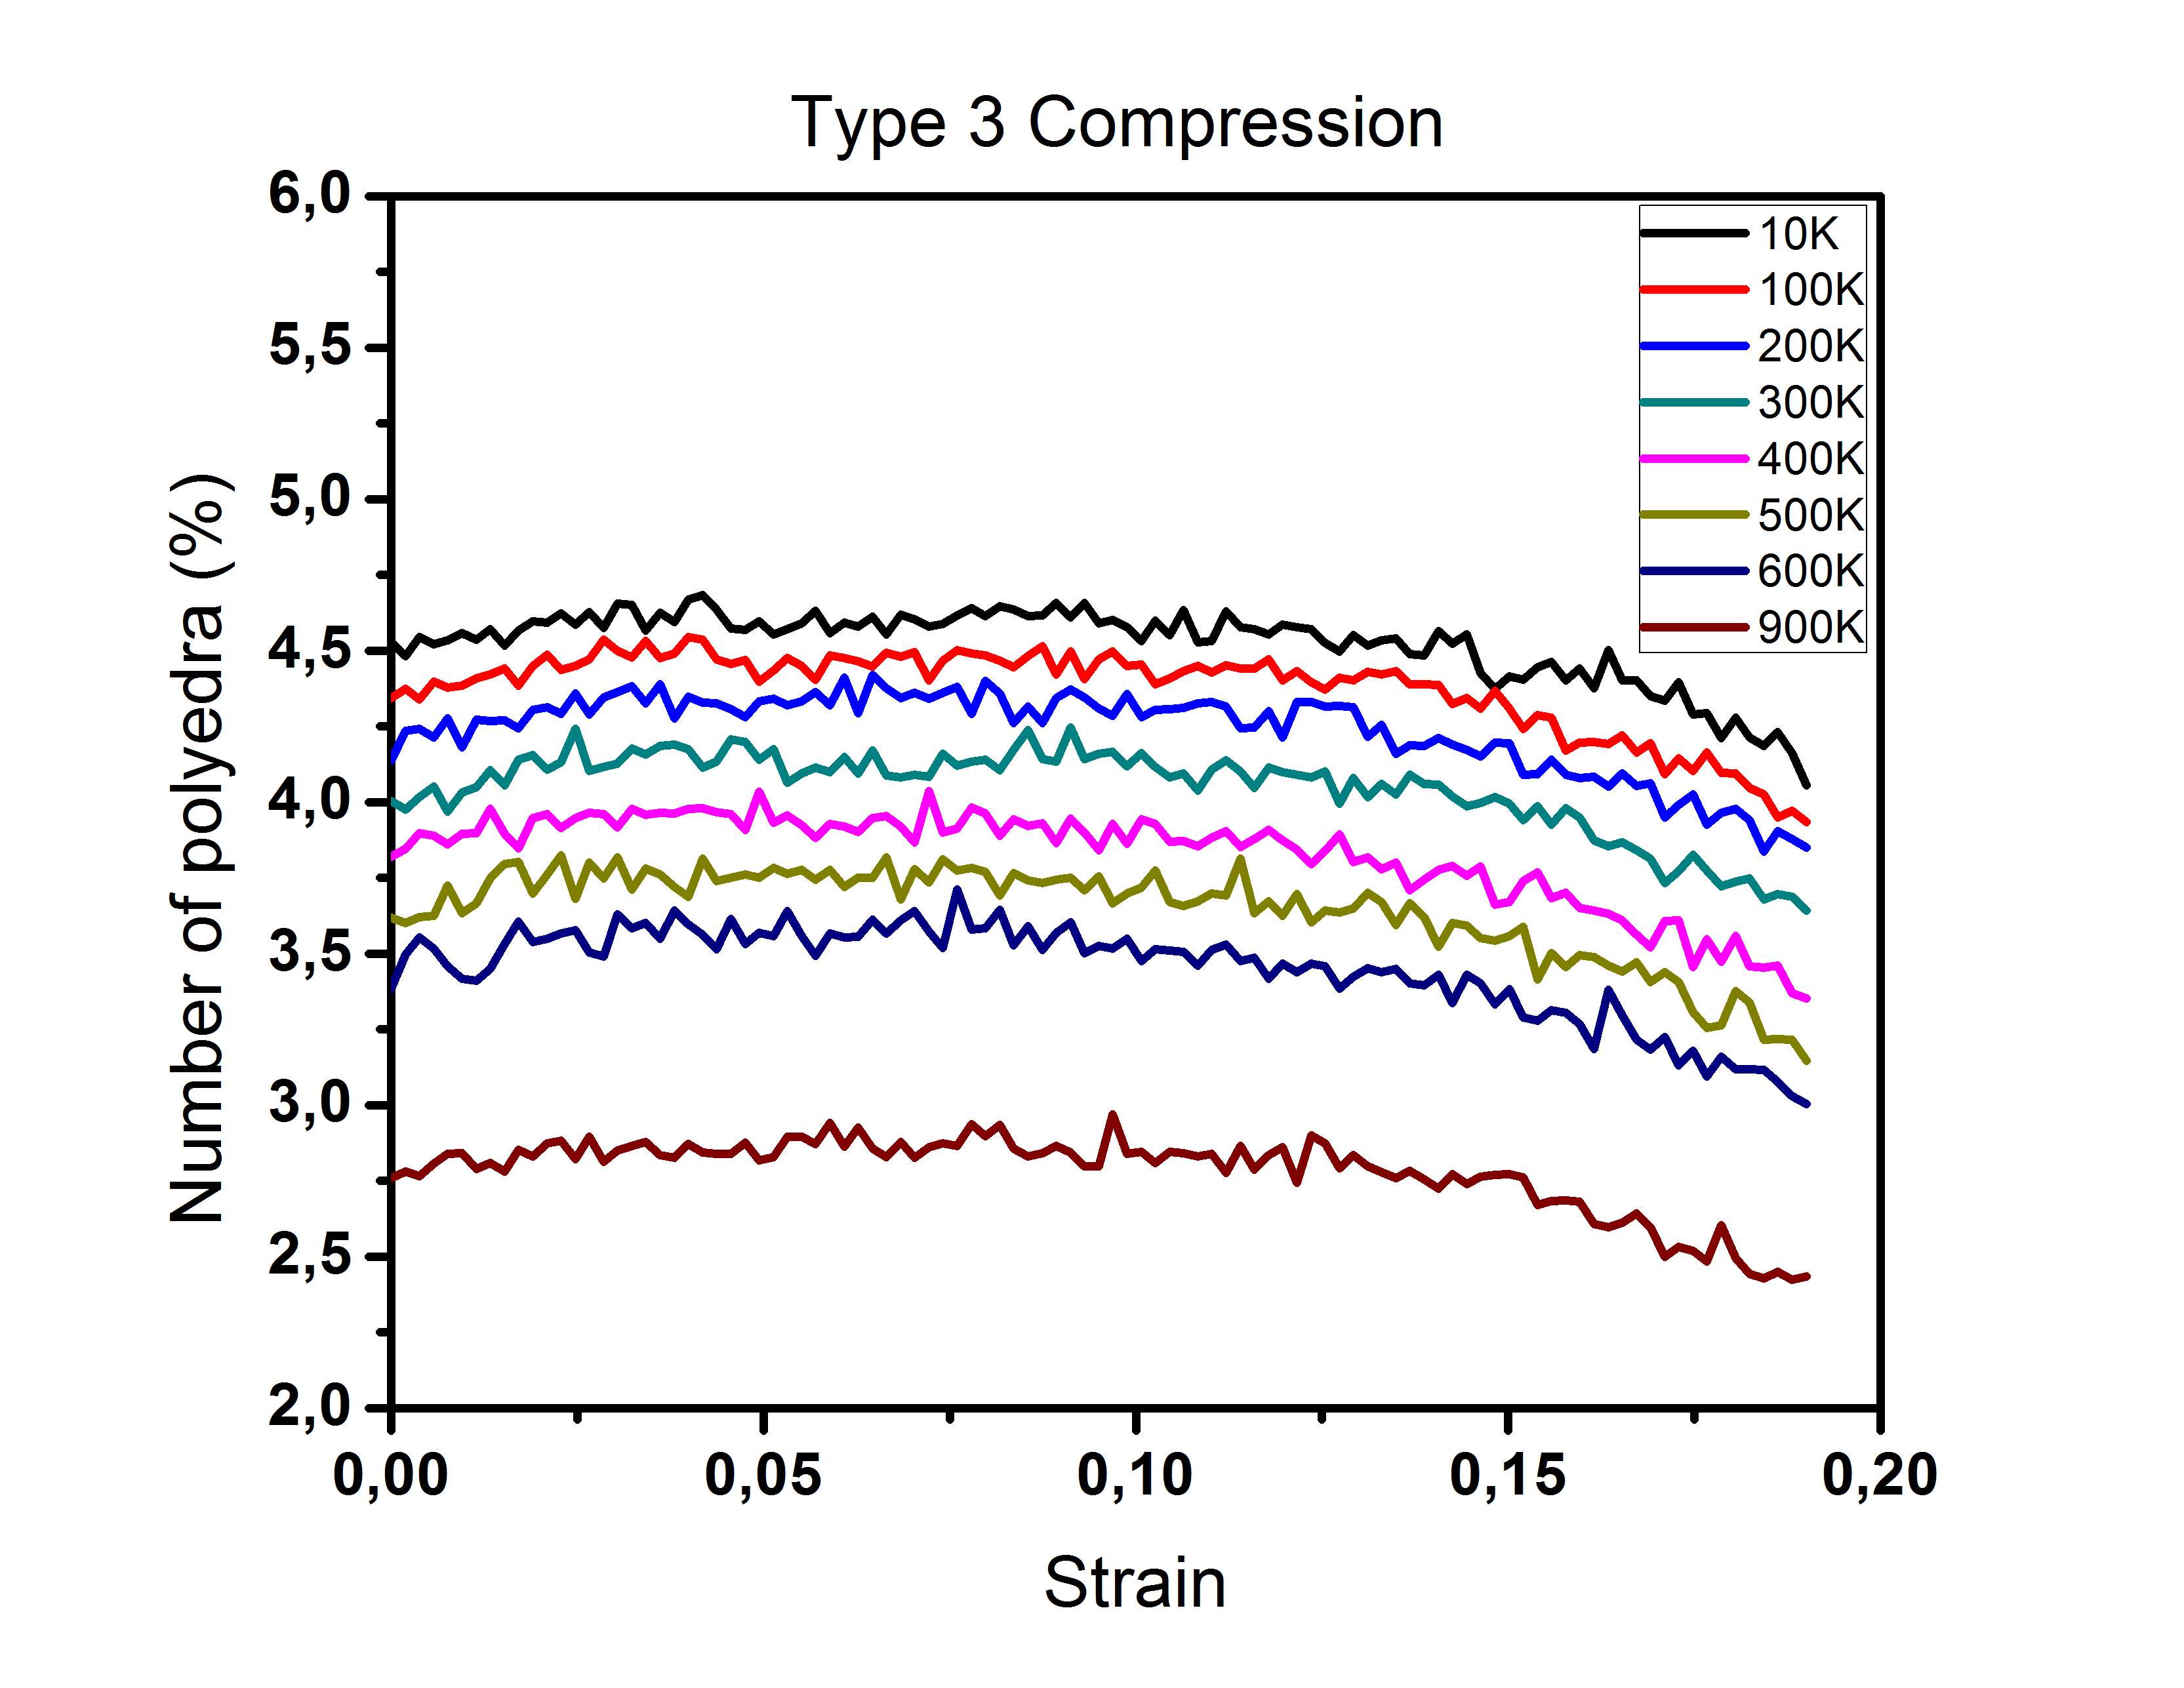
\includegraphics[width=8cm]{Figures/type3_COMP.png}
\caption{polyedros de voronoi tipo 3 vs. strain}
\end{figure}

\begin{figure}[H]
\centering
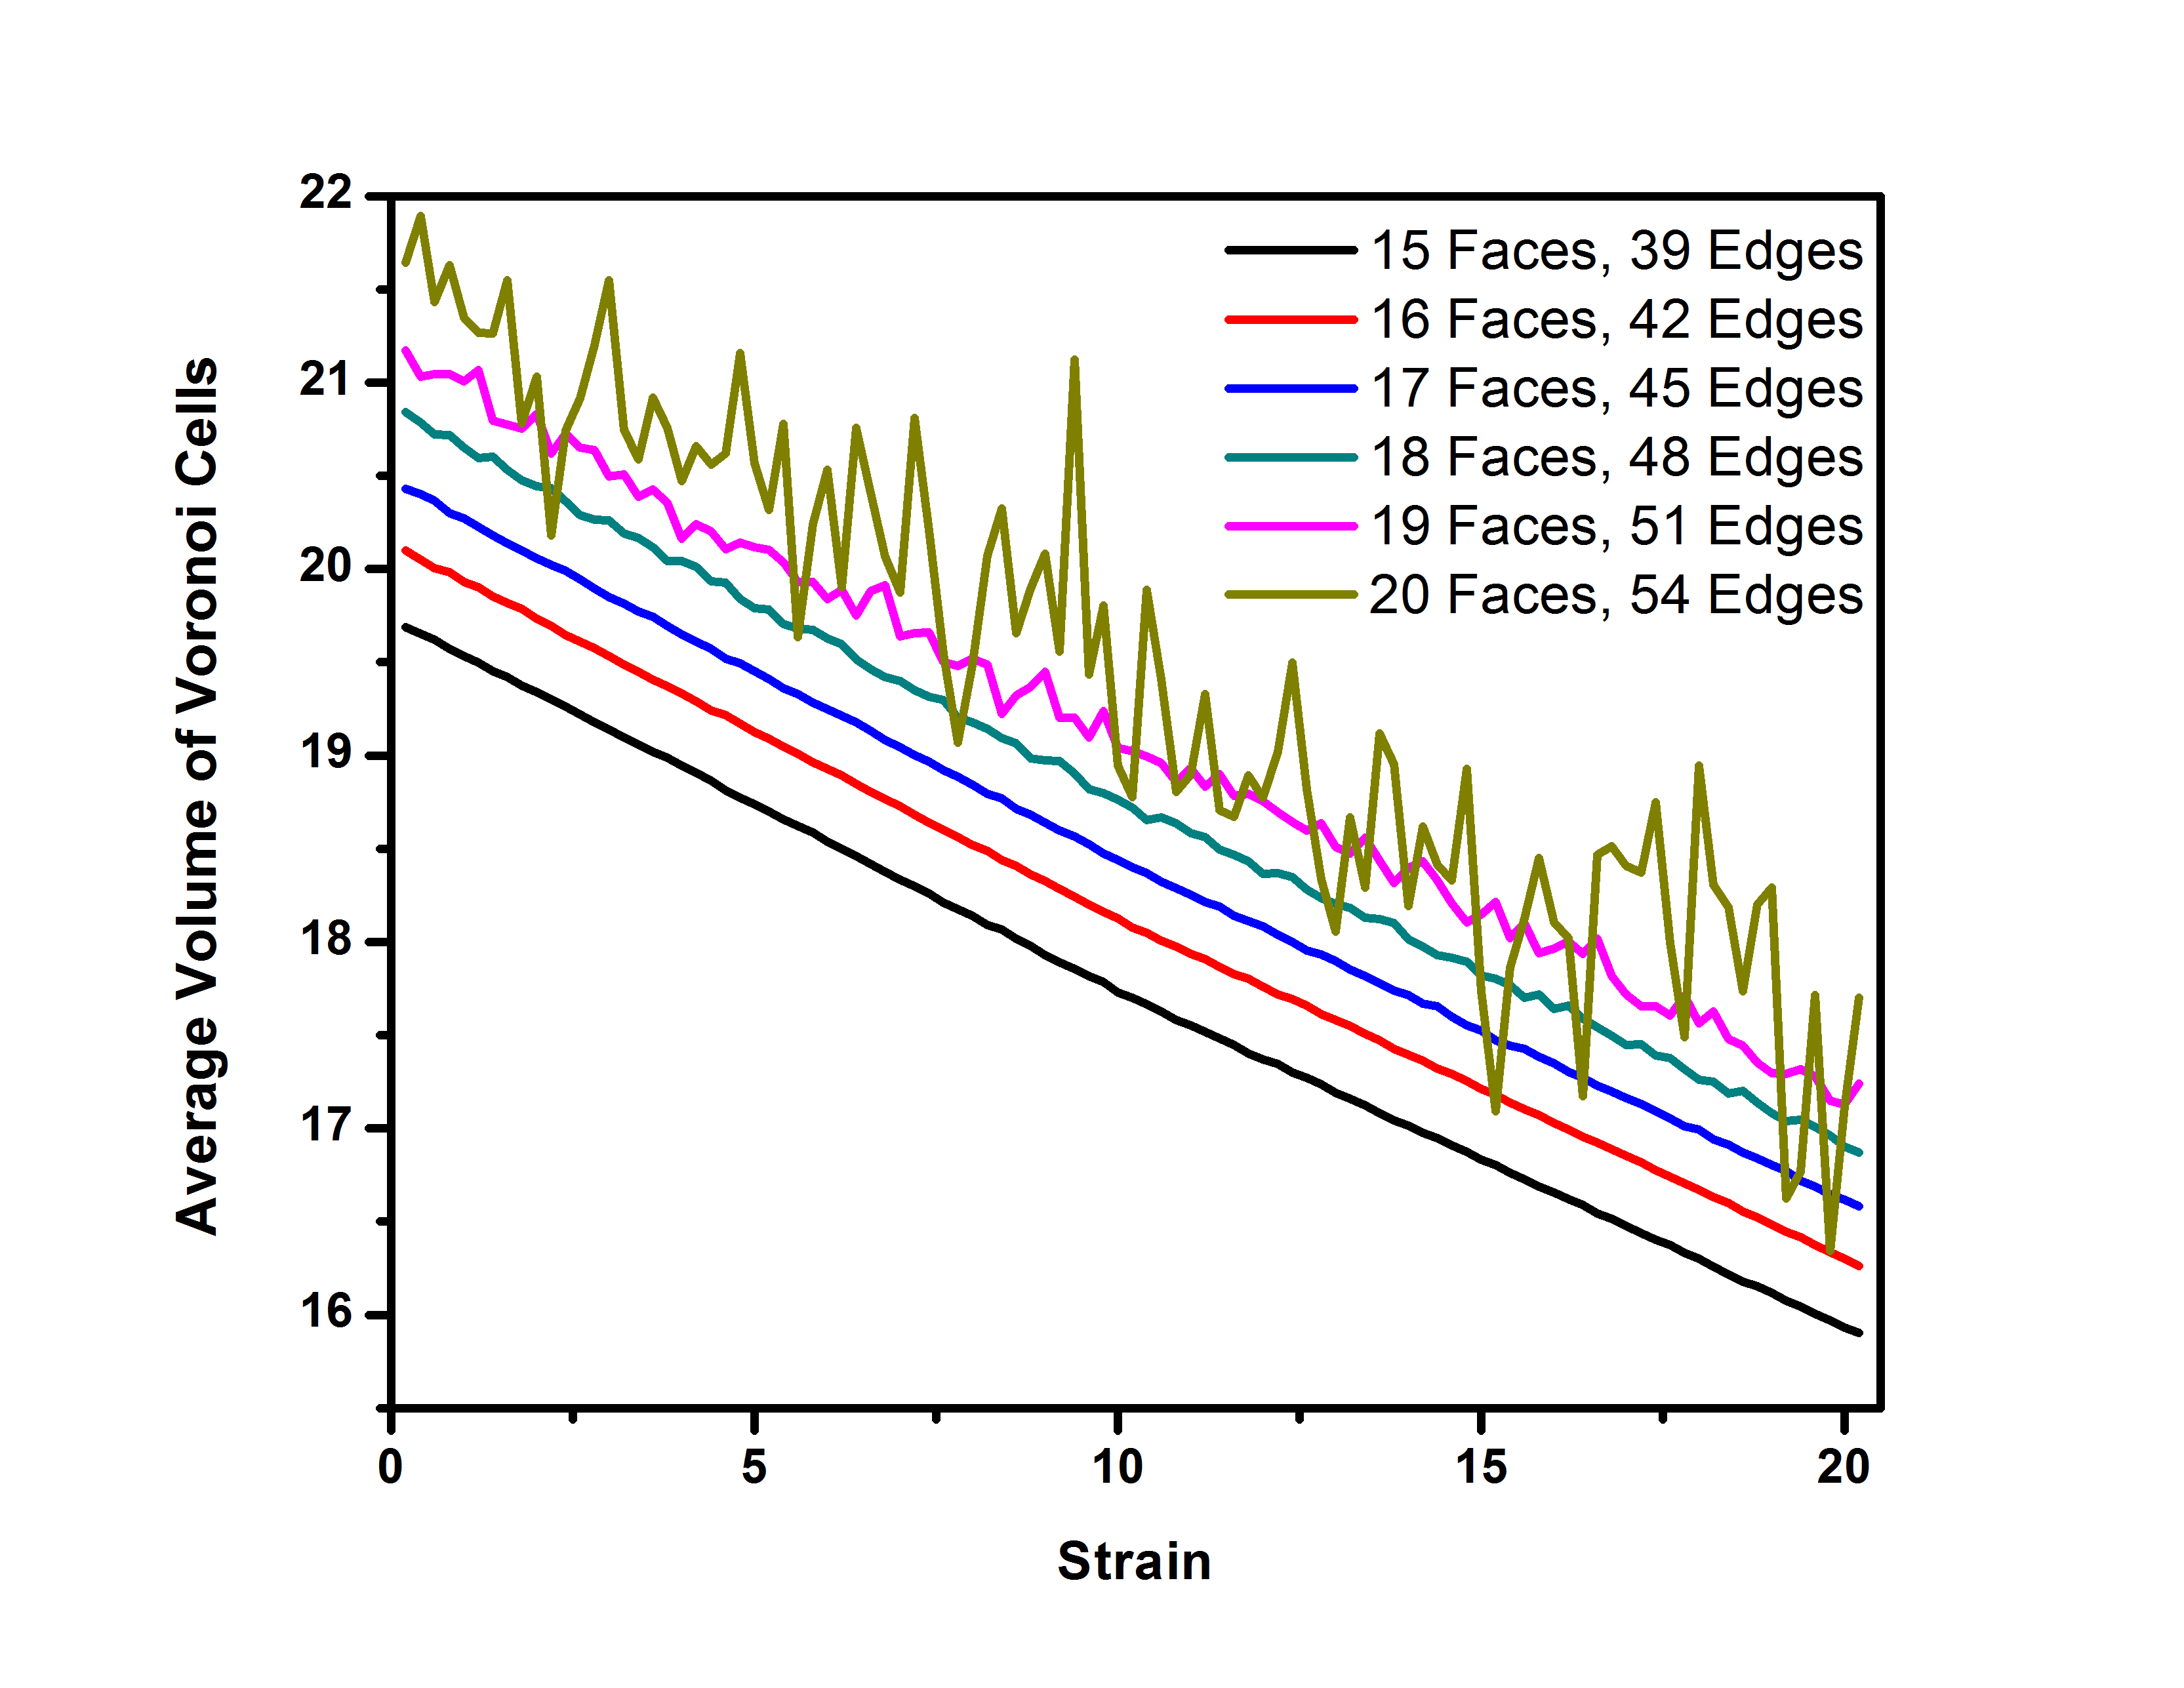
\includegraphics[width=8cm]{Figures/COMP_Vol_Step_A.png}
\caption{volumen promedio de voronoi cells (parte 1/2, temperatura desconocida)}
\end{figure}

\begin{figure}[H]
\centering
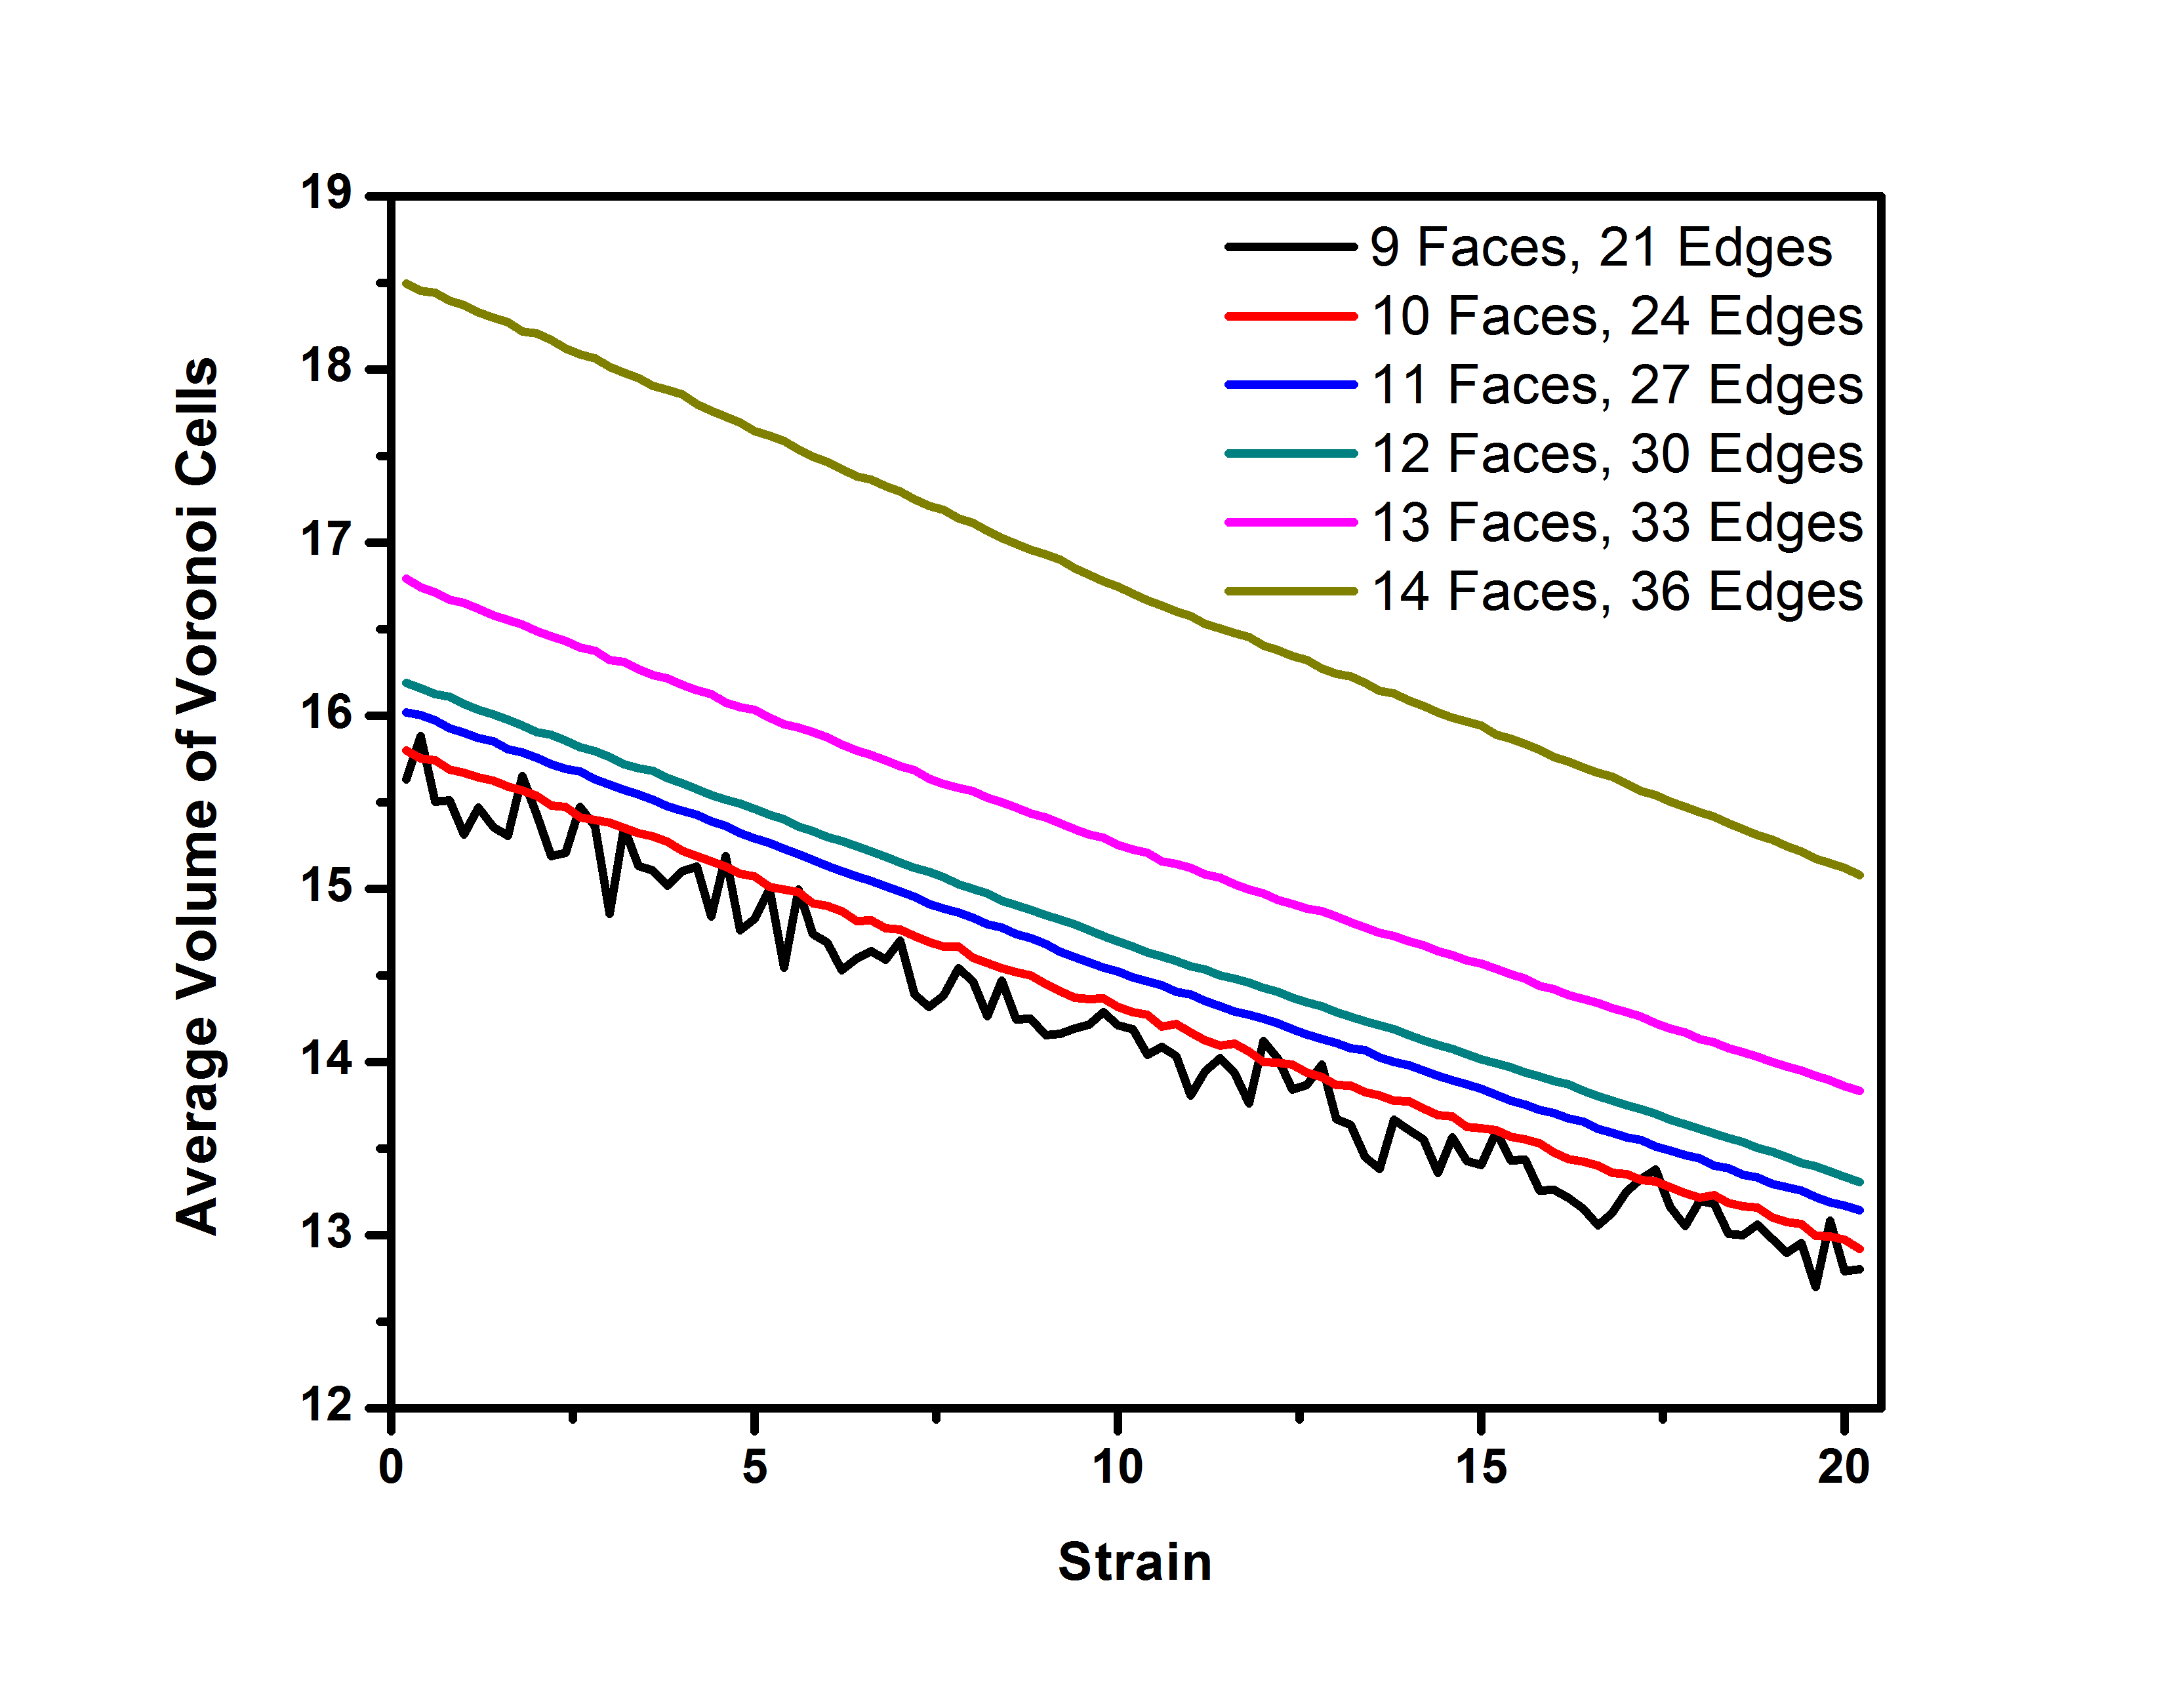
\includegraphics[width=8cm]{Figures/COMP_Vol_Step_B.png}
\caption{volumen promedio de voronoi cells (parte 2/2, temperatura desconocida)}
\end{figure}

\begin{figure}[H]
\centering
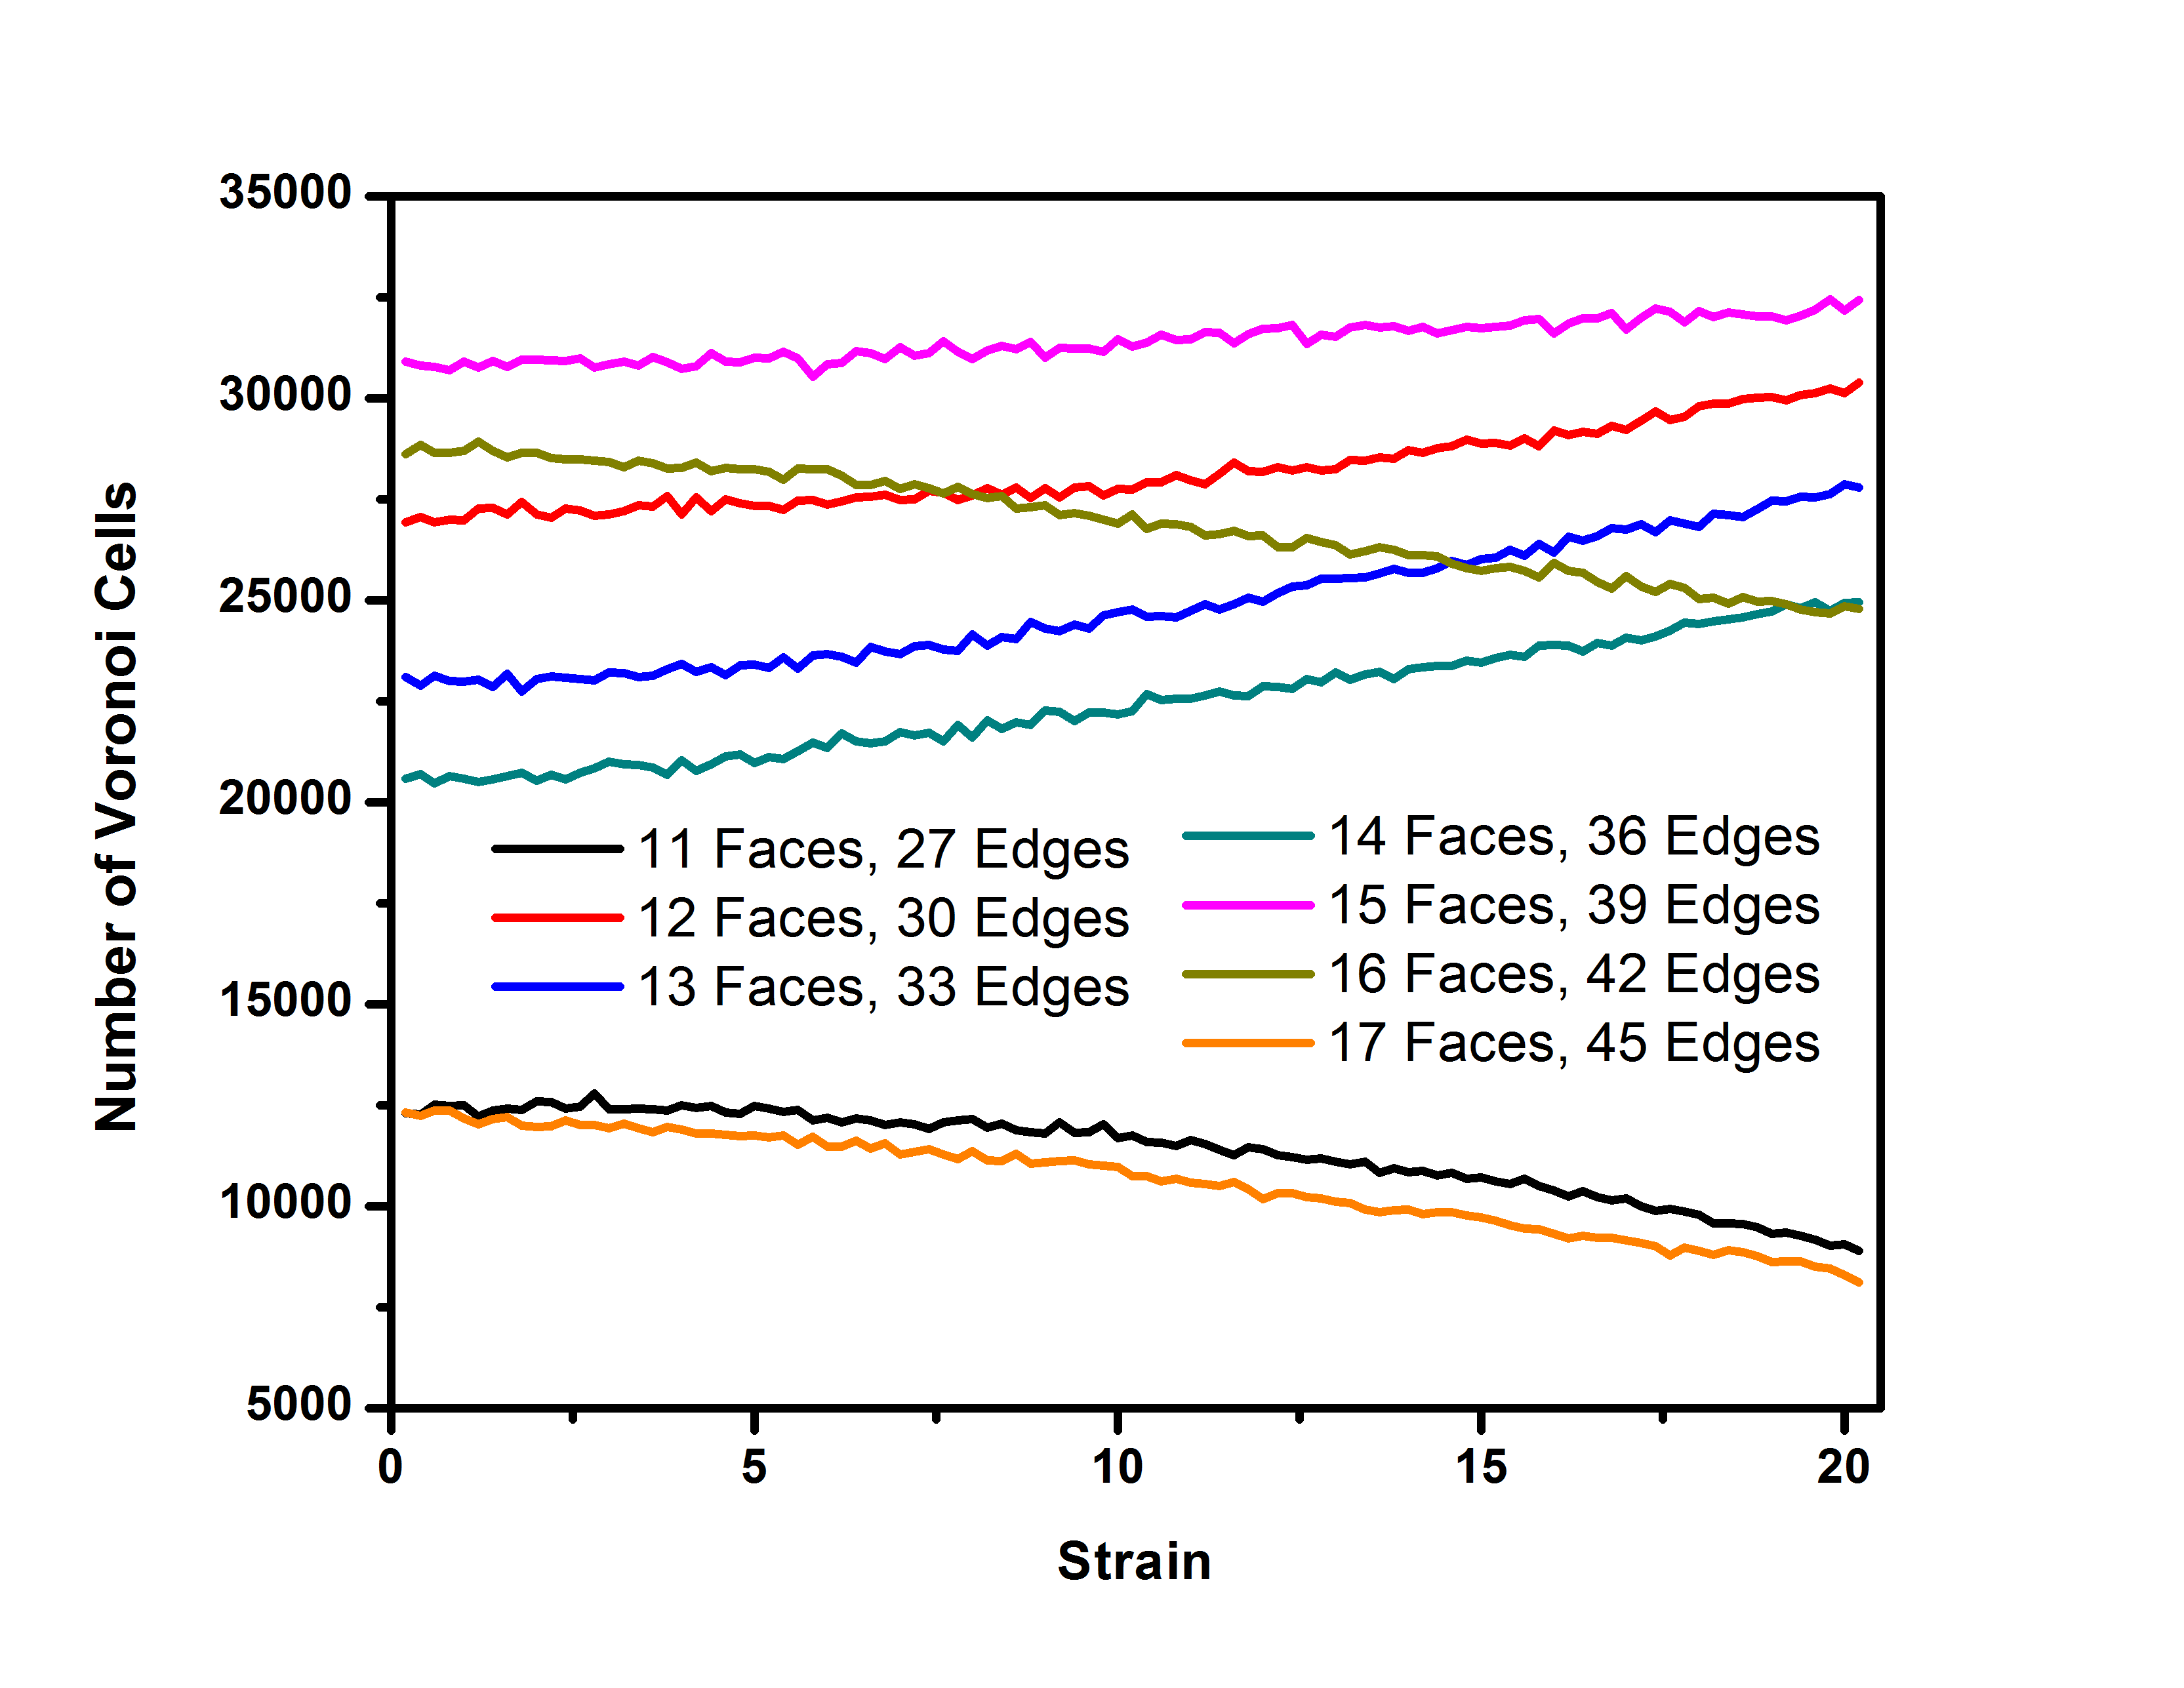
\includegraphics[width=8cm]{Figures/COMP_Num_Step.png}
\caption{numero celdas de voronoi (temperatura desconocida)}
\end{figure}

\begin{figure}[H]
\centering
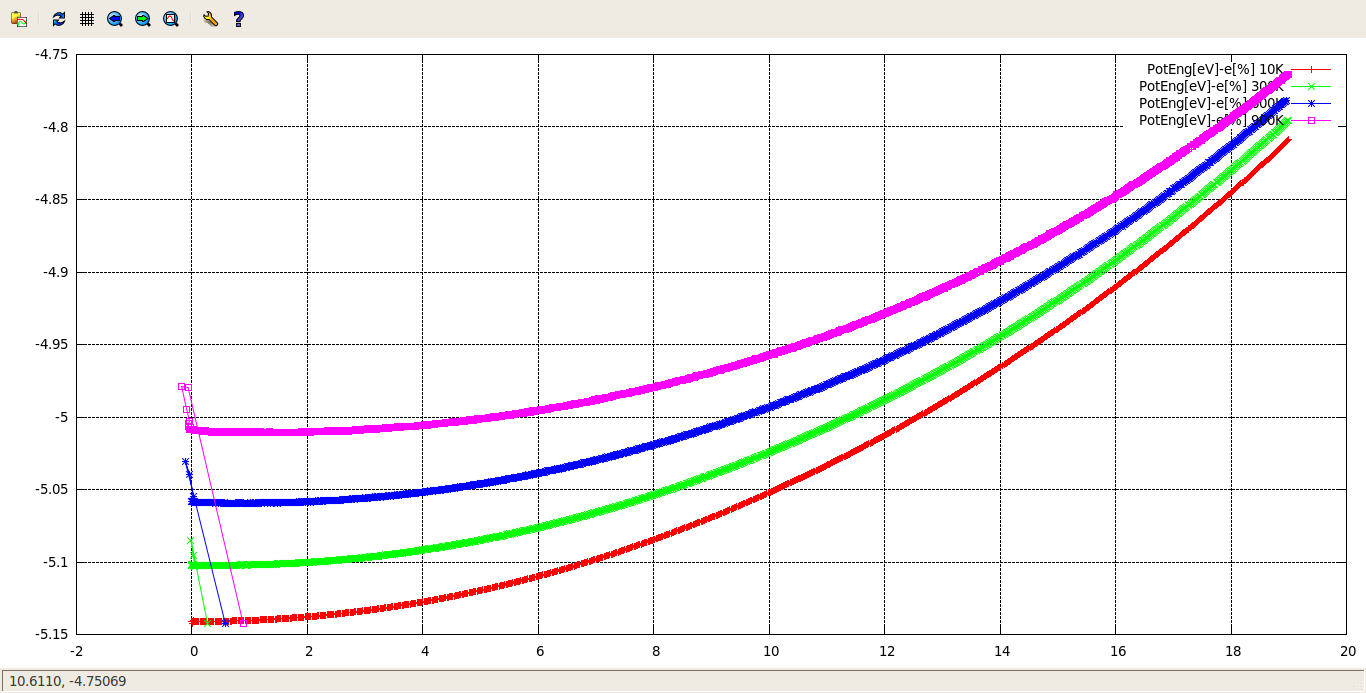
\includegraphics[width=8cm]{Figures/EngPot_COMP.png}
\caption{Energia potencial}
\end{figure}

\begin{figure}[H]
\centering
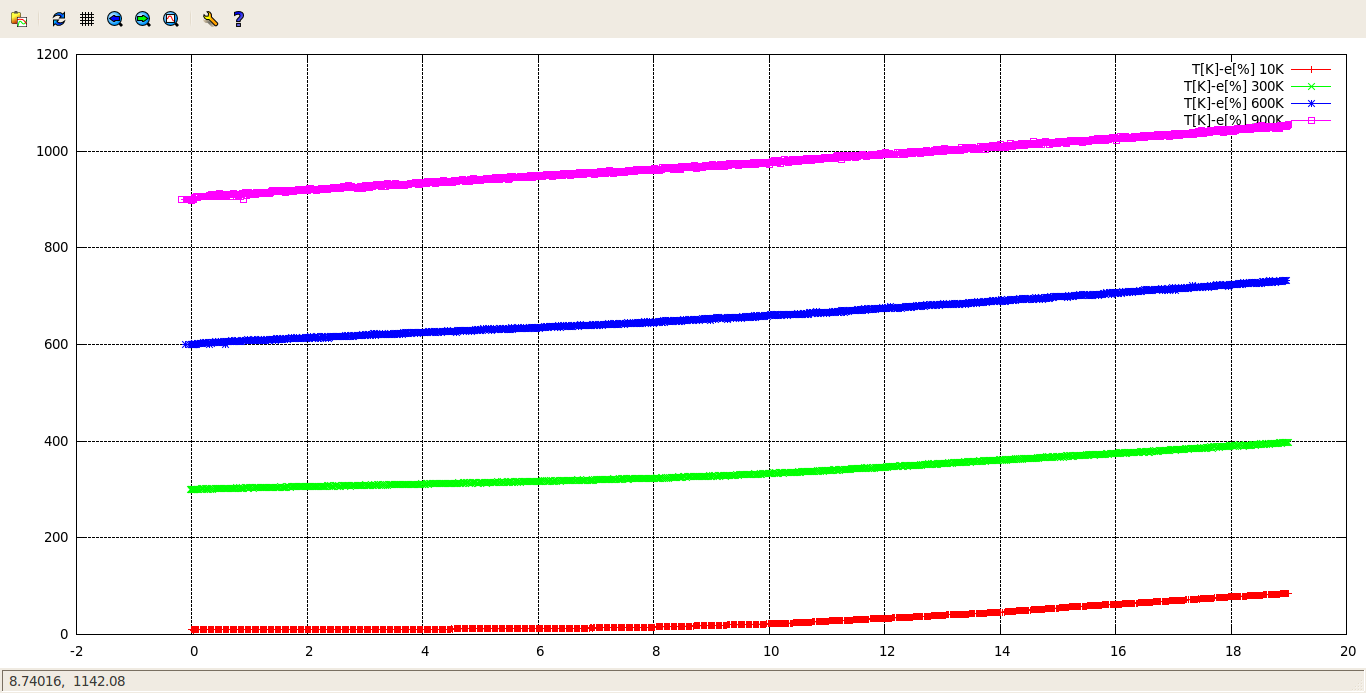
\includegraphics[width=8cm]{Figures/Temp_COMP.png}
\caption{Temperatura}
\end{figure}

\begin{figure}[H]
\centering
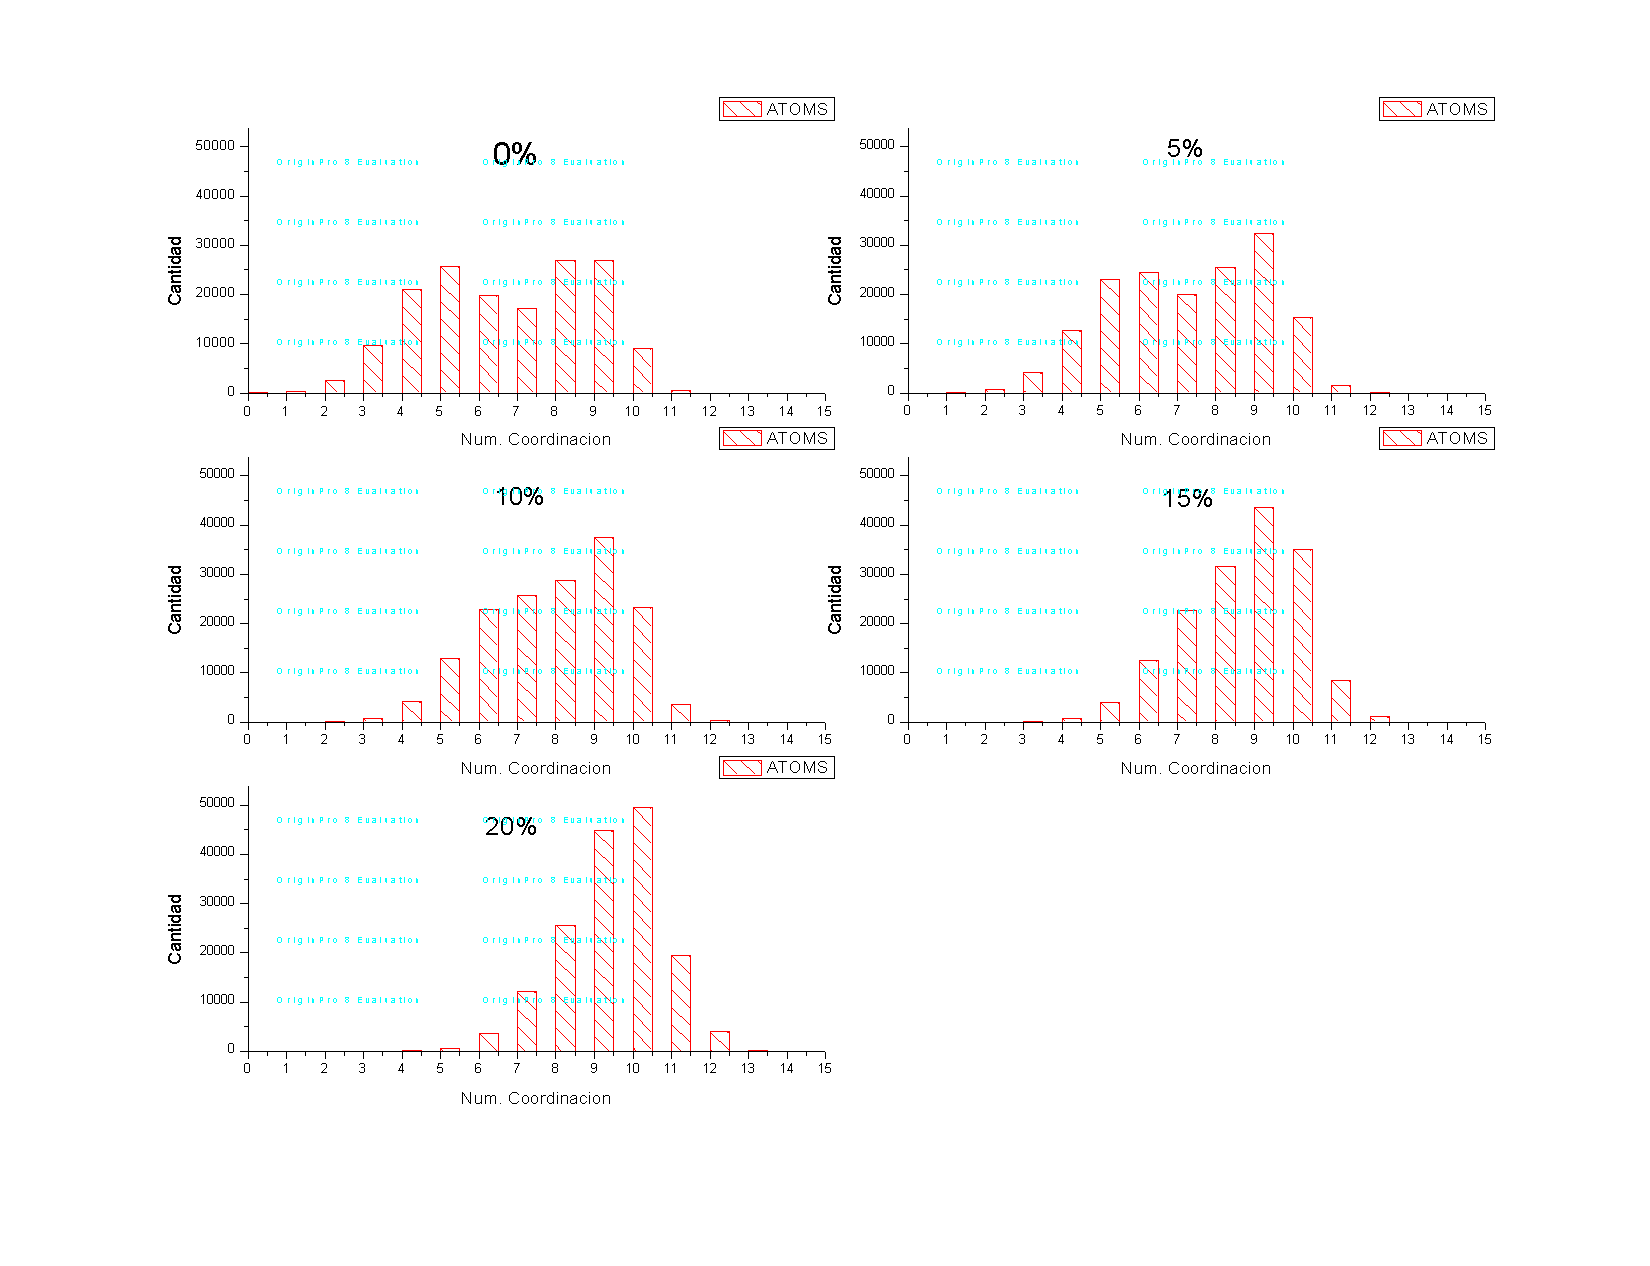
\includegraphics[width=16cm]{Figures/10-HistogramaCoord_COMP.png}
\caption{Histograma de numero de coordinacion a varios strains. 10K}
\end{figure}

\begin{figure}[H]
\centering
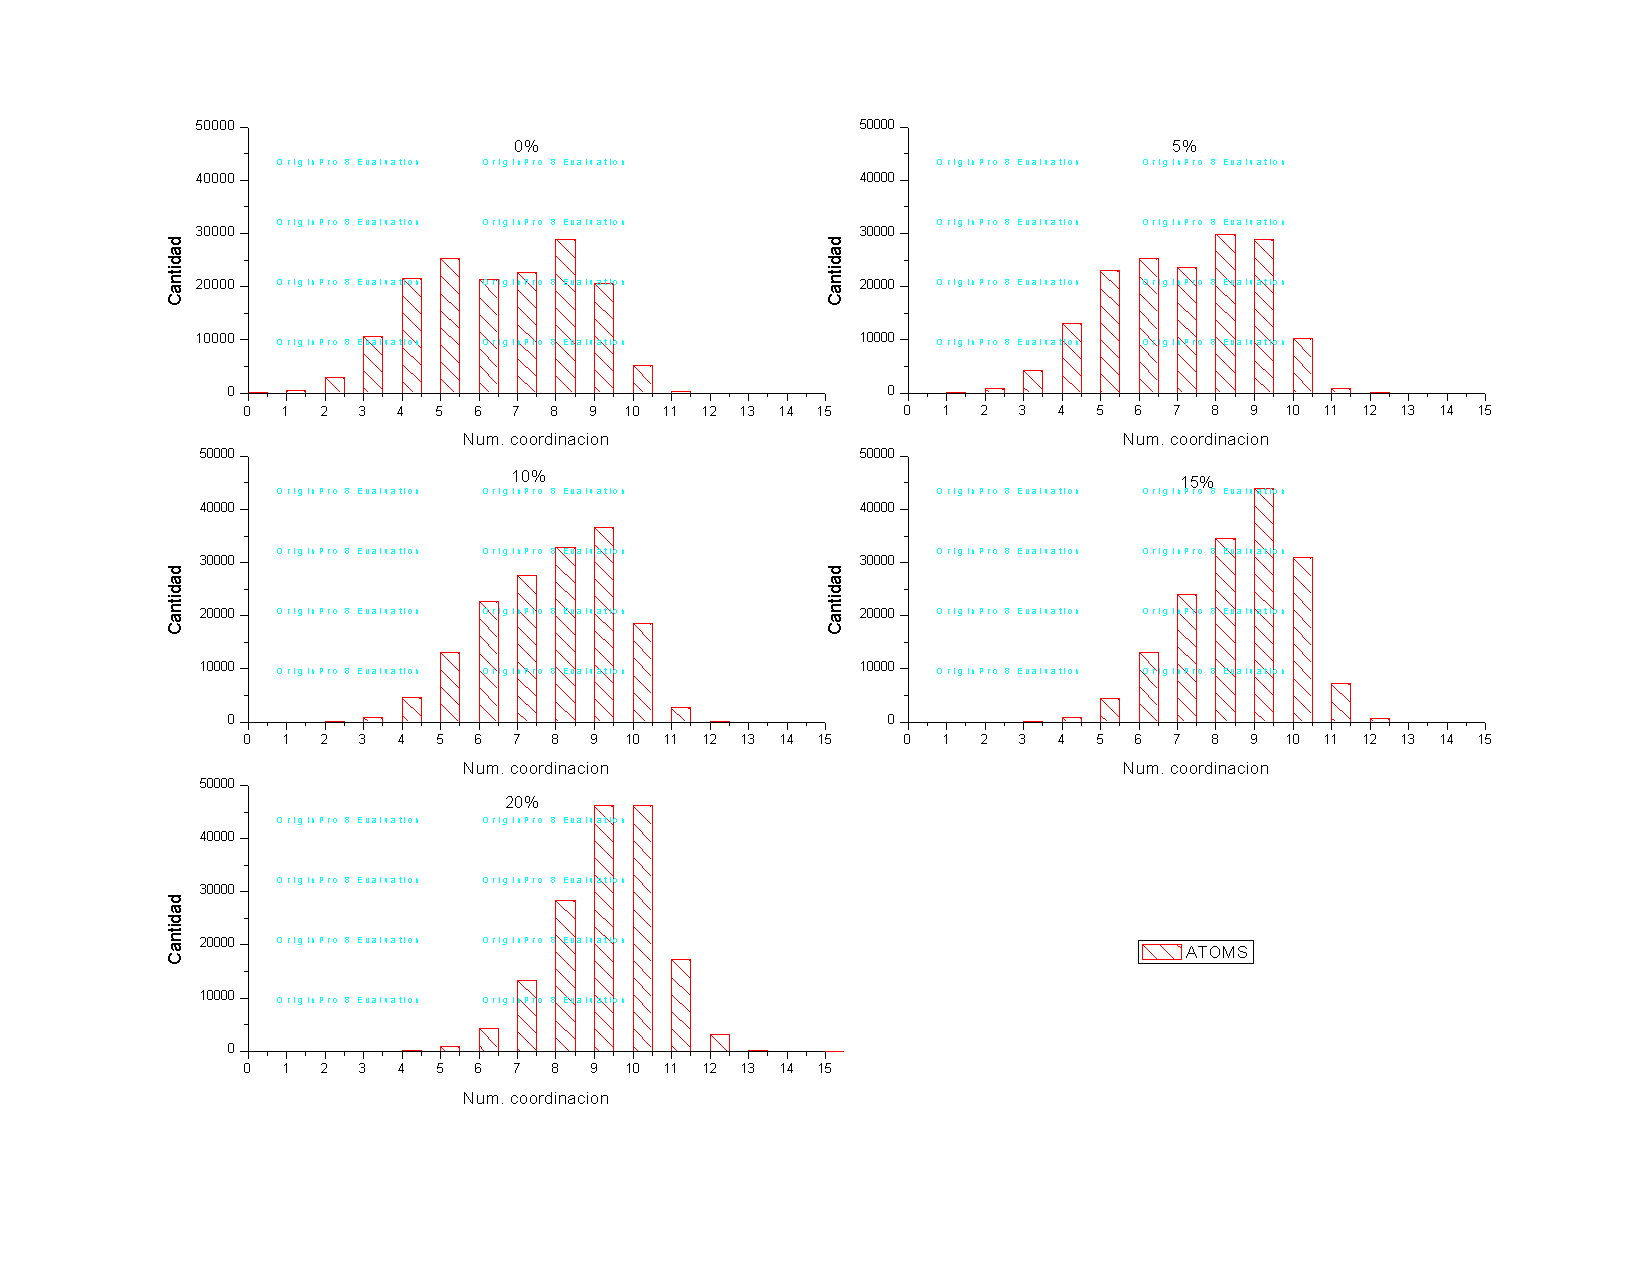
\includegraphics[width=16cm]{Figures/300-HistogramaCoord_COMP.png}
\caption{Histograma de numero de coordinacion a varios strains. 300K}
\end{figure}

\begin{figure}[H]
\centering
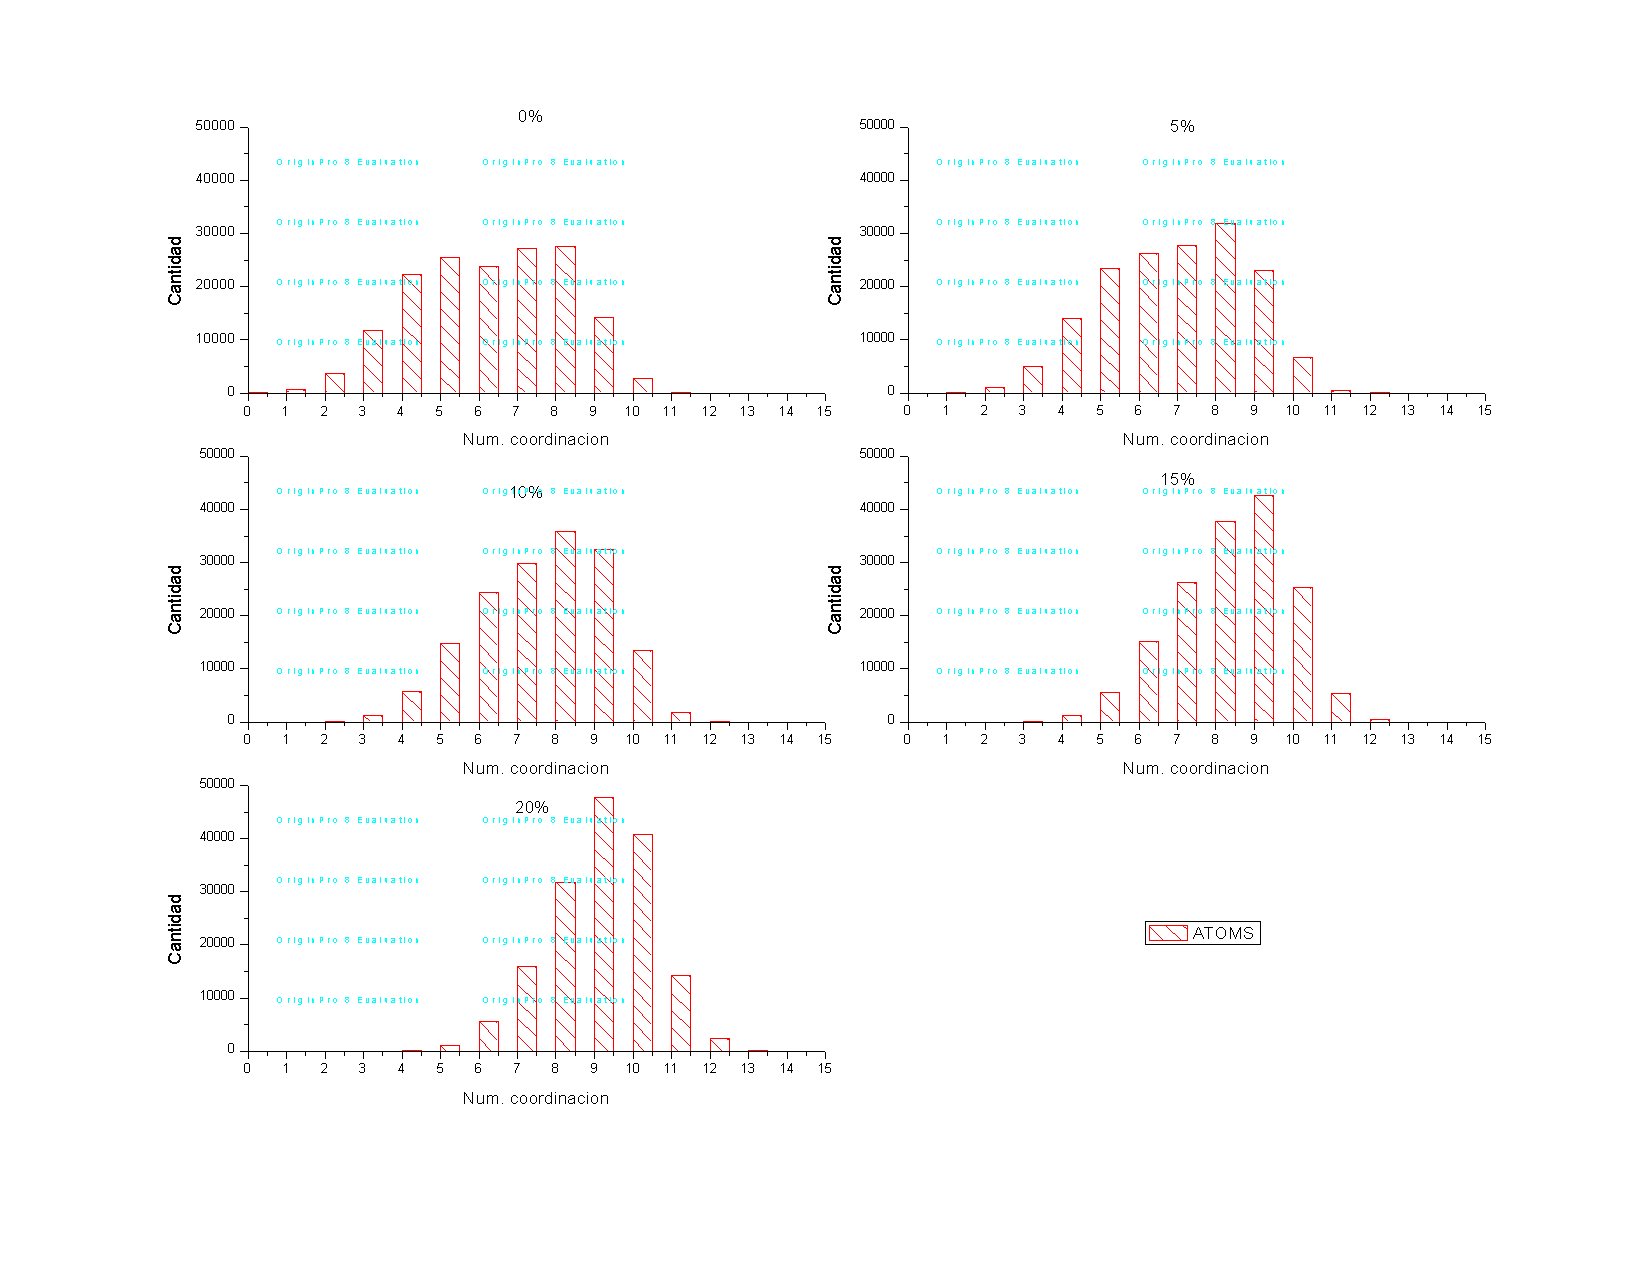
\includegraphics[width=16cm]{Figures/600-HistogramaCoord_COMP.png}
\caption{Histograma de numero de coordinacion a varios strains. 600K}
\end{figure}

\begin{figure}[H]
\centering
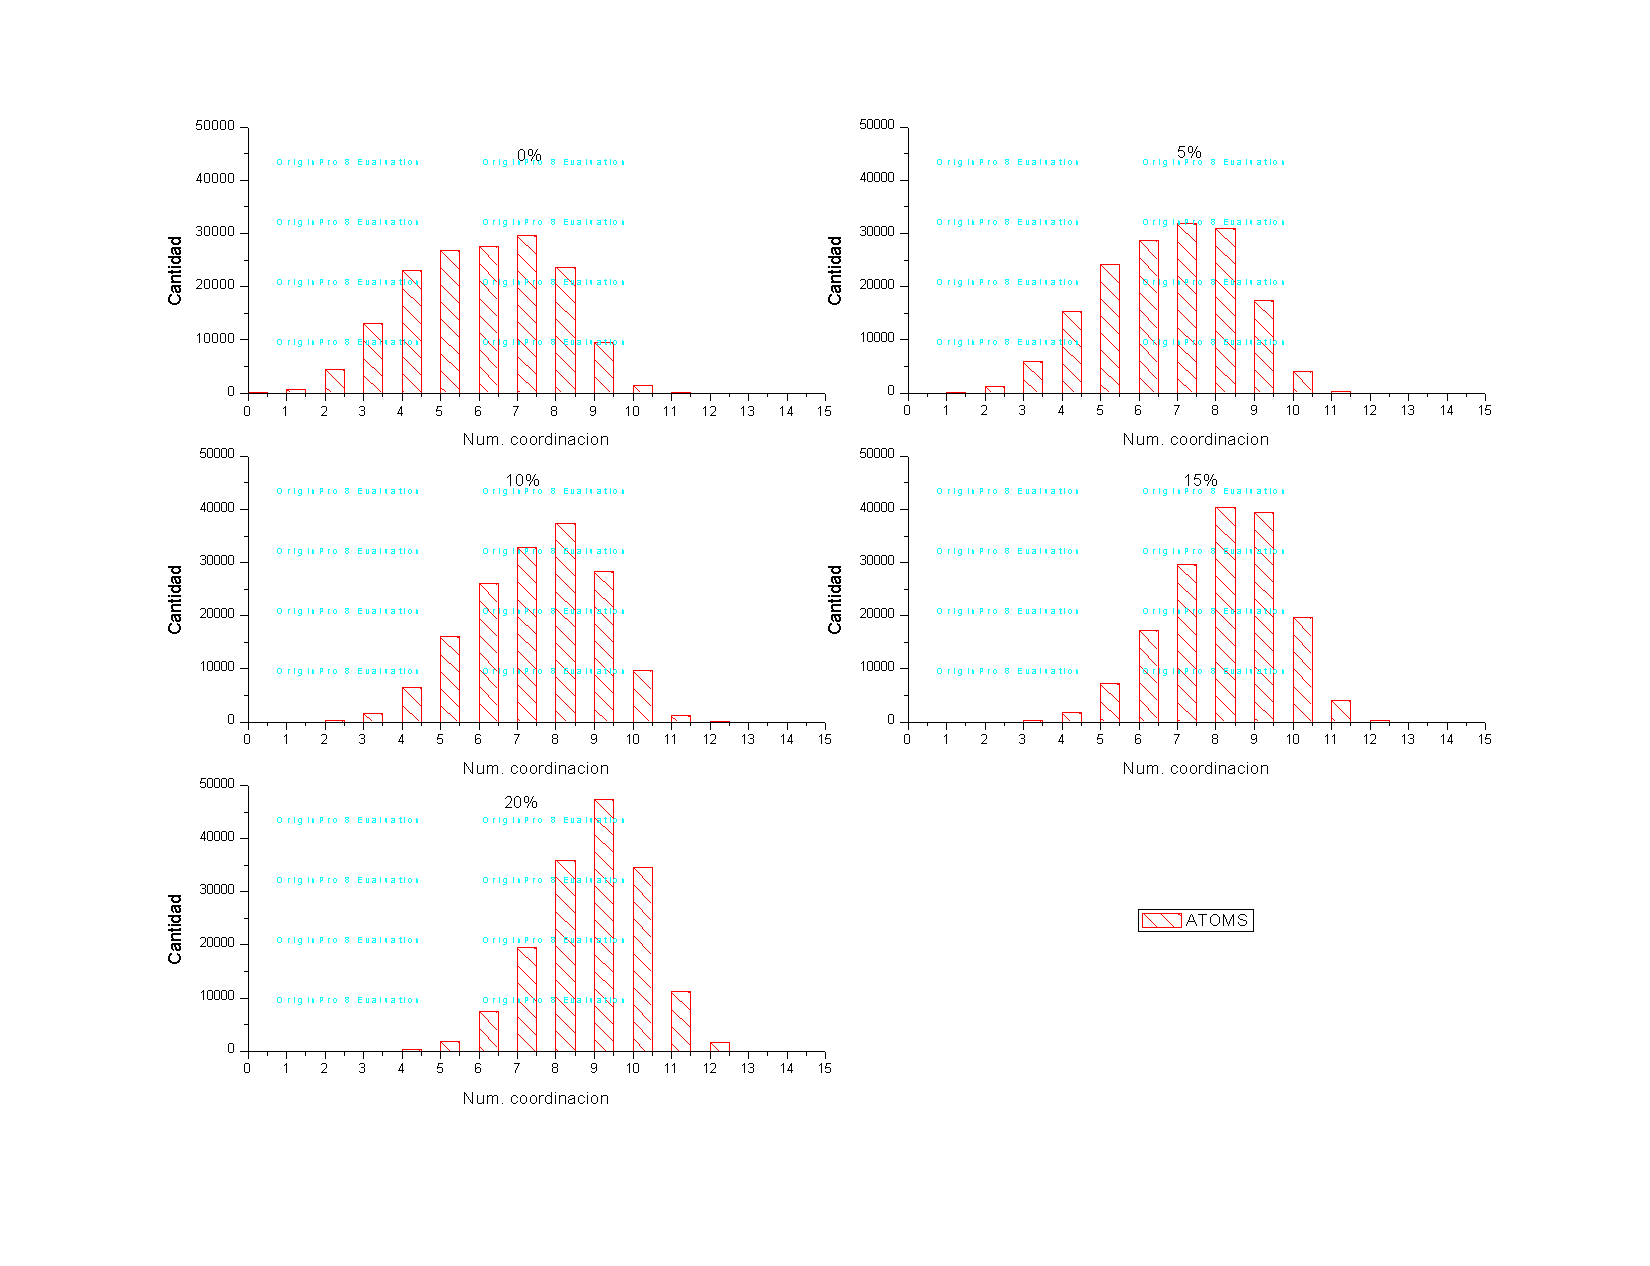
\includegraphics[width=16cm]{Figures/900-HistogramaCoord_COMP.png}
\caption{Histograma de numero de coordinacion a varios strains. 900K}
\end{figure}

\begin{lstlisting}[caption=script para relajacion]
 # 3d Uniaxial 
 
read_restart tmp.restart.50000

pair_style	eam/alloy 
pair_coeff	* *  ZrCu_lammps.eam Cu Zr 

compute cke all ke/atom
compute cpe all pe/atom
compute cstr all stress/atom pair
compute ccoord all coord/atom 3.0

thermo 100
thermo_style custom step temp ke pe etotal press pxx pyy pzz pxy pxz pyz ly lx lz 
thermo_modify	lost warn norm yes

reset_timestep	0

fix	INTEGRATE_FIX  all nve

dump OUT1 all custom 2500 dump_All_relajacion_*.lammpstrj x y z c_ccoord c_cpe c_cke
    vx vy vz id type c_cstr[1] c_cstr[2] c_cstr[3] c_cstr[4] c_cstr[5] c_cstr[6] 
restart	        50000 tmp.restart.relajacion.* 
thermo 100

fix DEFORM_FIX   all deform 1 z erate 0.001
timestep	0.002
run 50000
\end{lstlisting}

\begin{figure}[H]
\centering
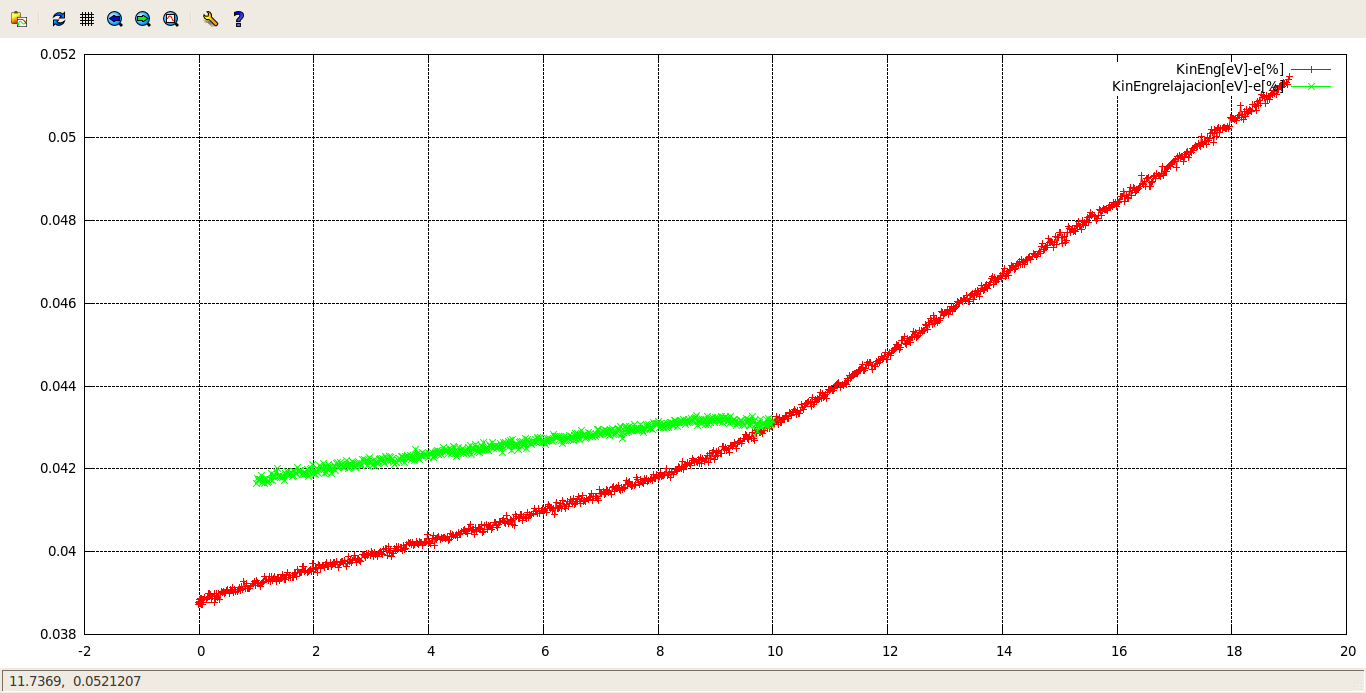
\includegraphics[width=10cm]{Figures/300_Relax_KinEng-deformacion_COMP.png}
\caption{Simulacion relajacion. 300K. Energia cinetica vs strain}
\end{figure}

\begin{figure}[H]
\centering
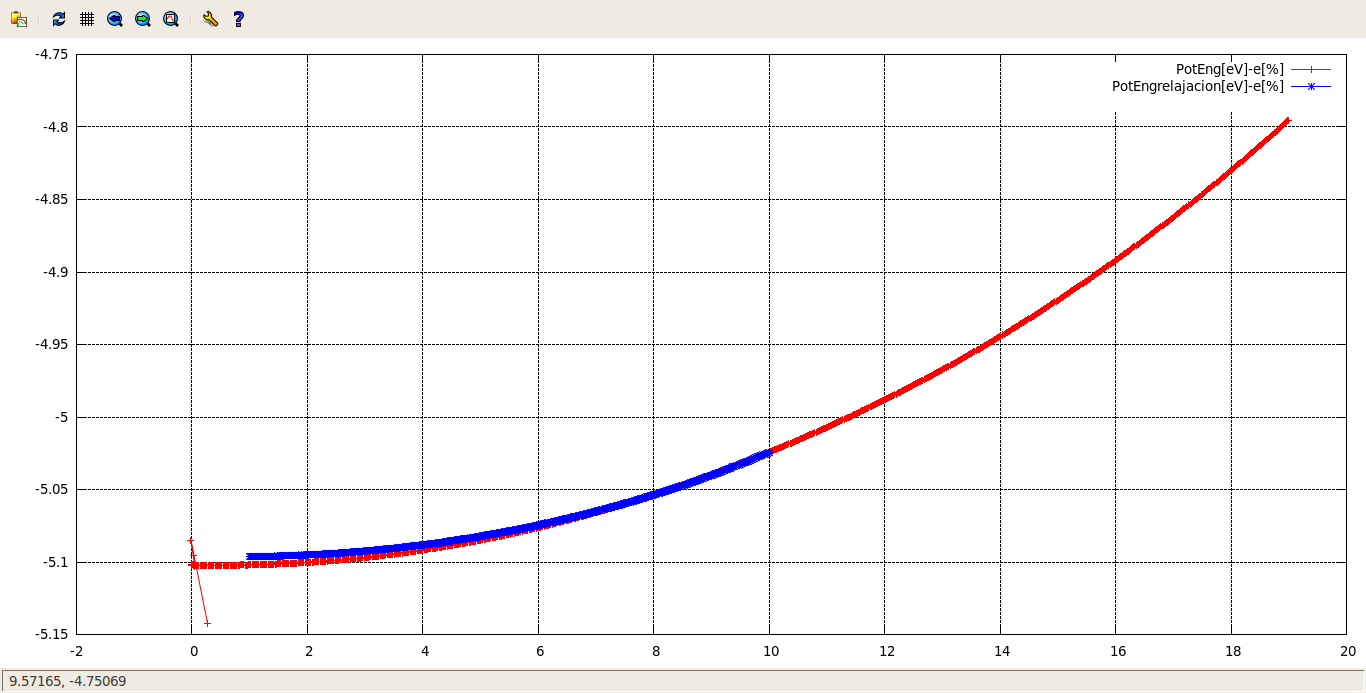
\includegraphics[width=10cm]{Figures/300_Relax_PotEng-deformacion_COMP.png}
\caption{Simulacion relajacion. 300K. Energia potencial vs strain}
\end{figure}

\begin{figure}[H]
\centering
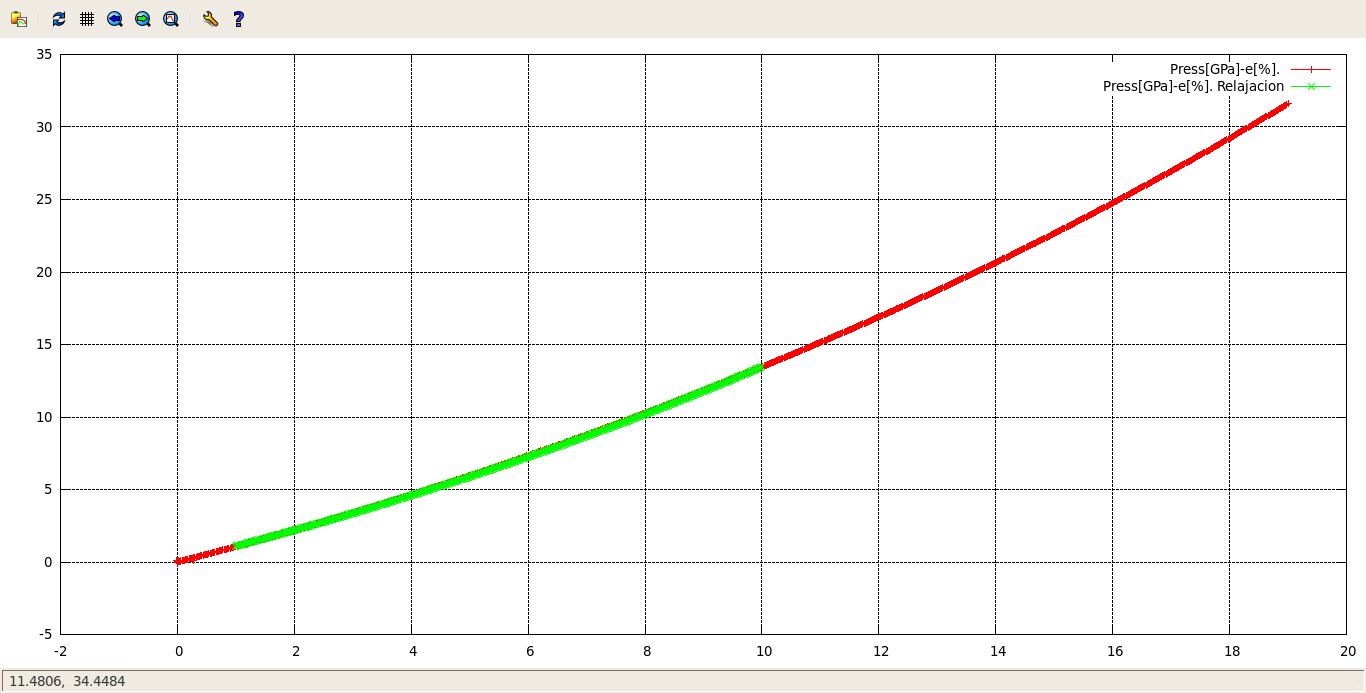
\includegraphics[width=10cm]{Figures/300_Relax_Press_COMP.png}
\caption{Simulacion relajacion. 300K. Press vs strain}
\end{figure}

\begin{figure}[H]
\centering
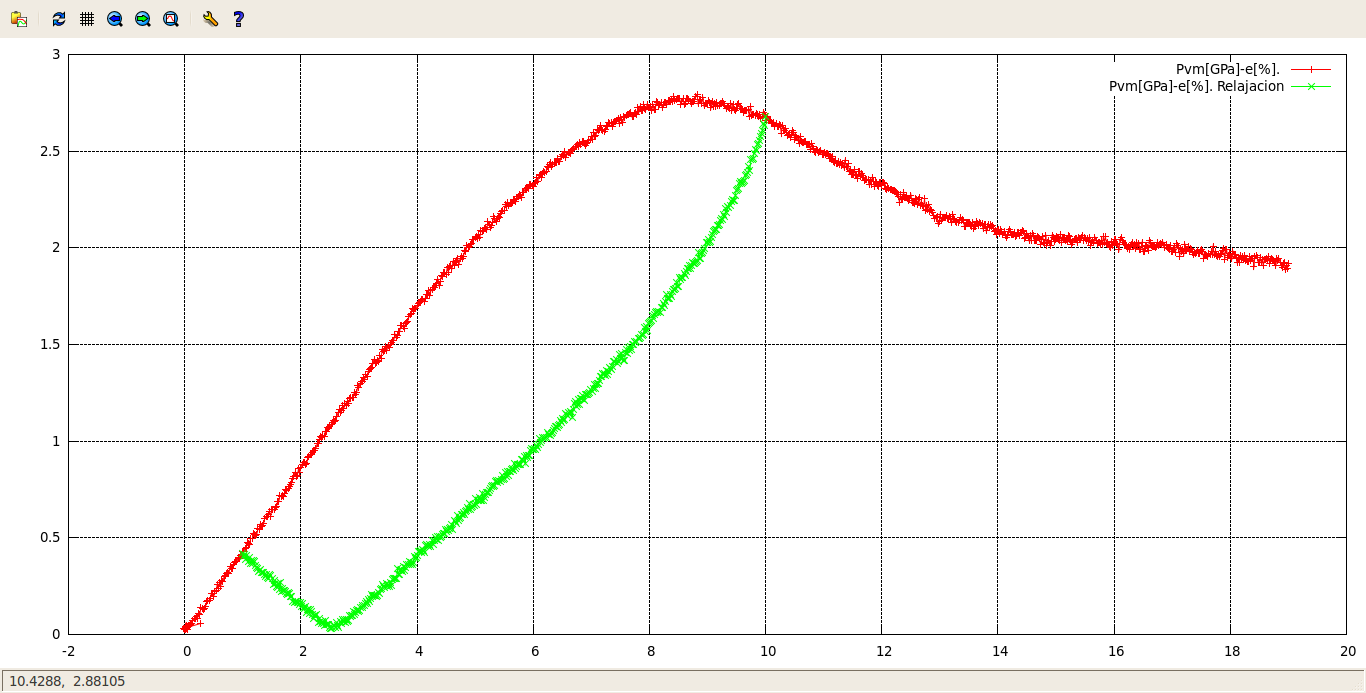
\includegraphics[width=10cm]{Figures/300_Relax_PVM-e_COMP.png}
\caption{Simulacion relajacion. 300K. Presion vonMises vs strain}
\end{figure}

\begin{figure}[H]
\centering
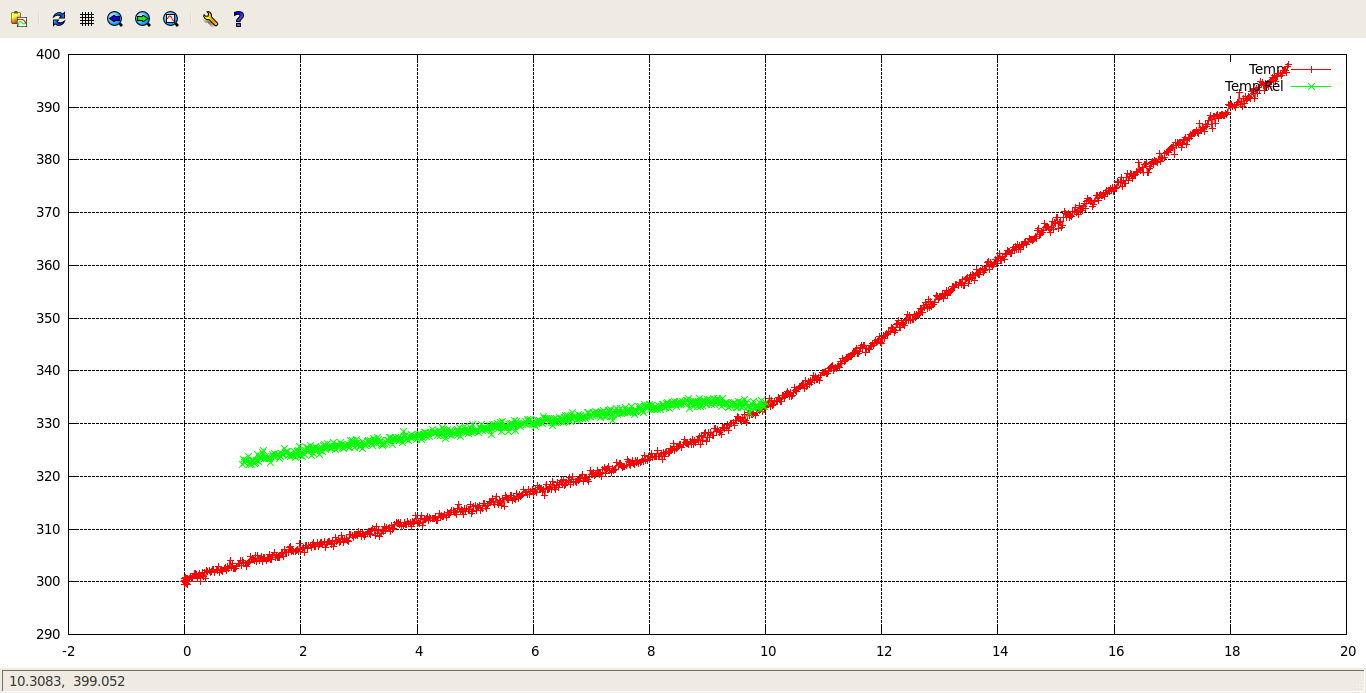
\includegraphics[width=10cm]{Figures/300_Relax_Temp_COMP.png}
\caption{Simulacion relajacion. 300K. Temperatura vs strain}
\end{figure}

\begin{figure}[H]
\centering
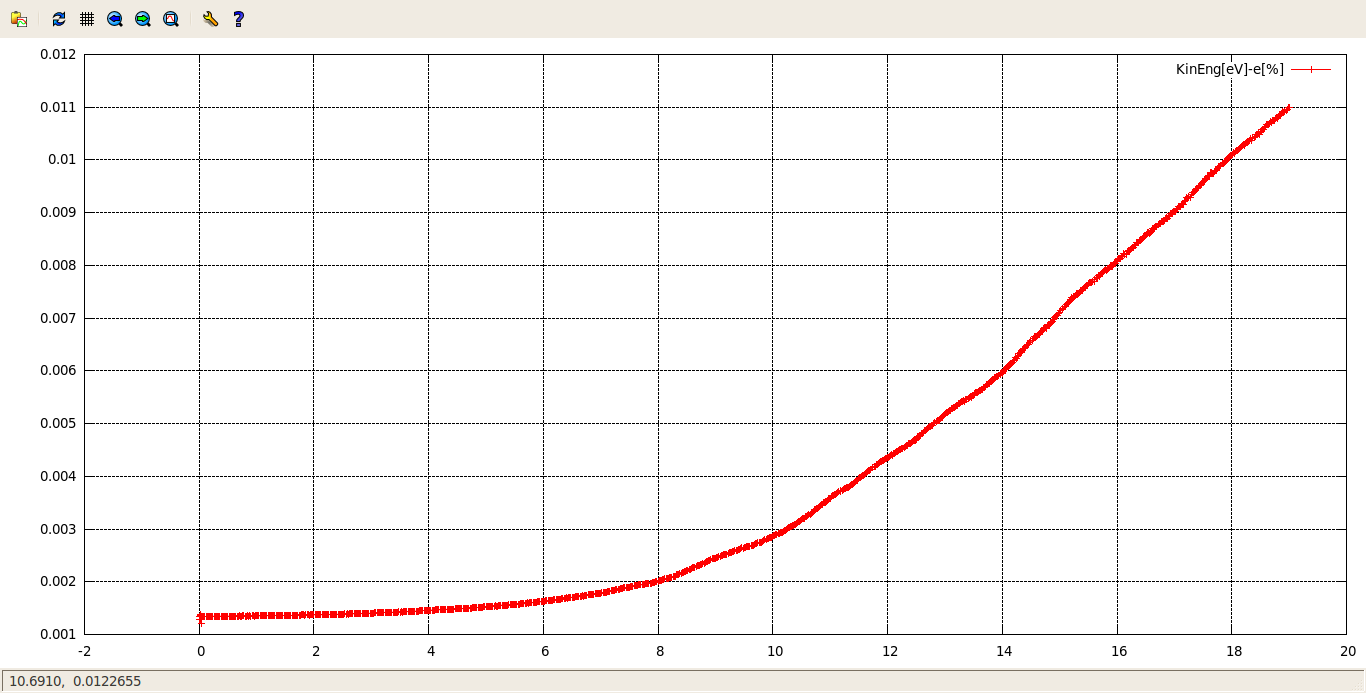
\includegraphics[width=8cm]{Figures/10-KinEng-deformacion.png}
\caption{10K. Energia cinetica vs strain}
\end{figure}

\begin{figure}[H]
\centering
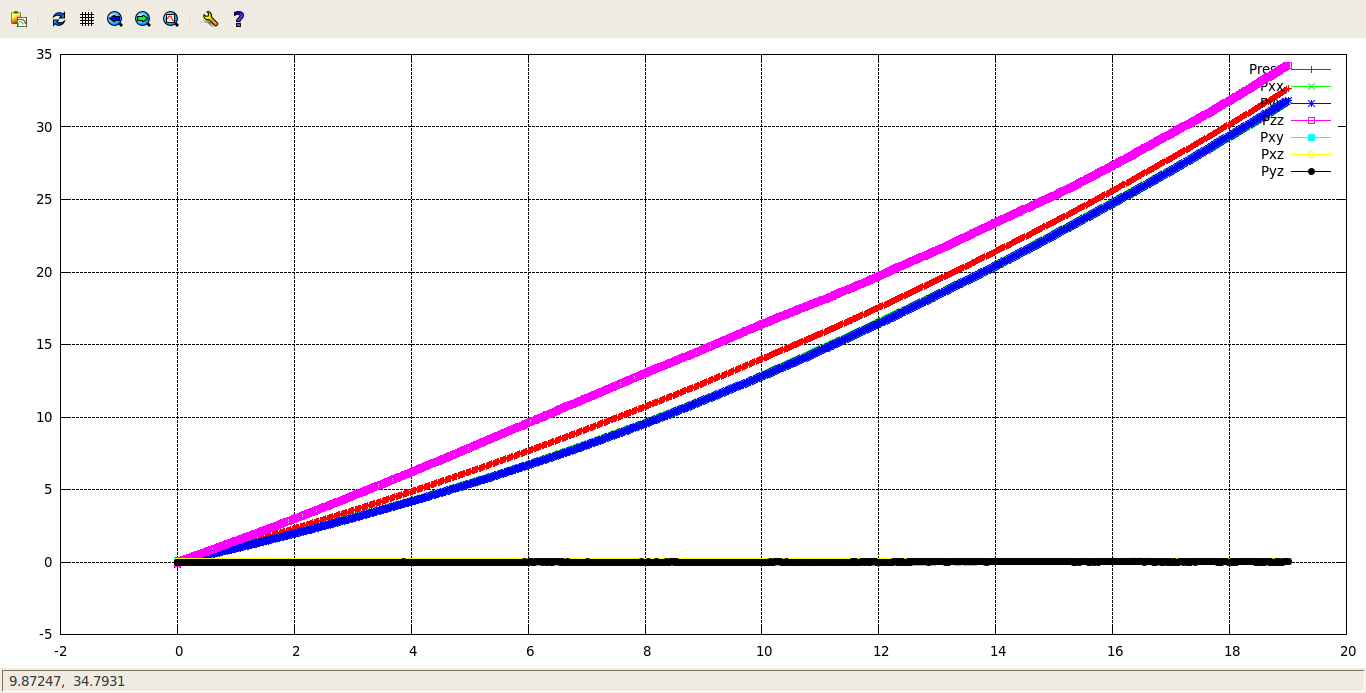
\includegraphics[width=8cm]{Figures/10-Tensiones-deformacion.png}
\caption{10K. Presiones vs strain}
\end{figure}

\begin{figure}[H]
\centering
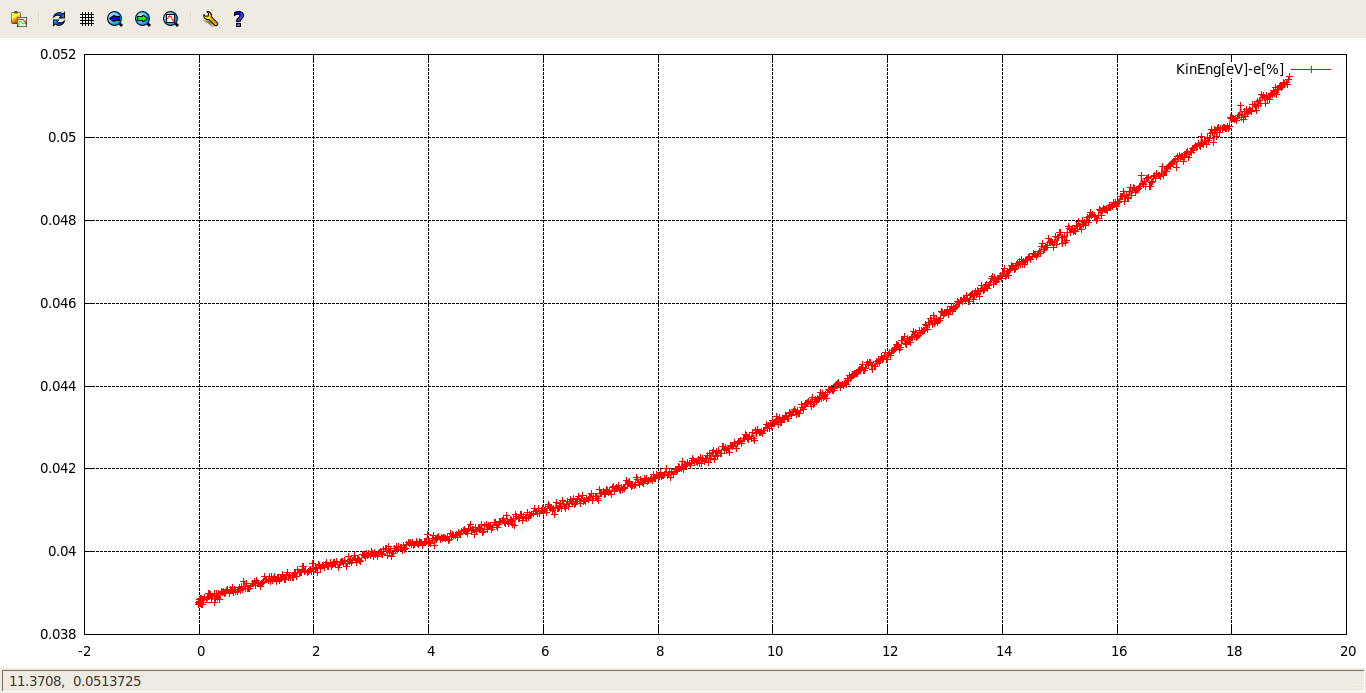
\includegraphics[width=8cm]{Figures/300-KinEng-deformacion.png}
\caption{300K. Energia cinetica vs strain}
\end{figure}

\begin{figure}[H]
\centering
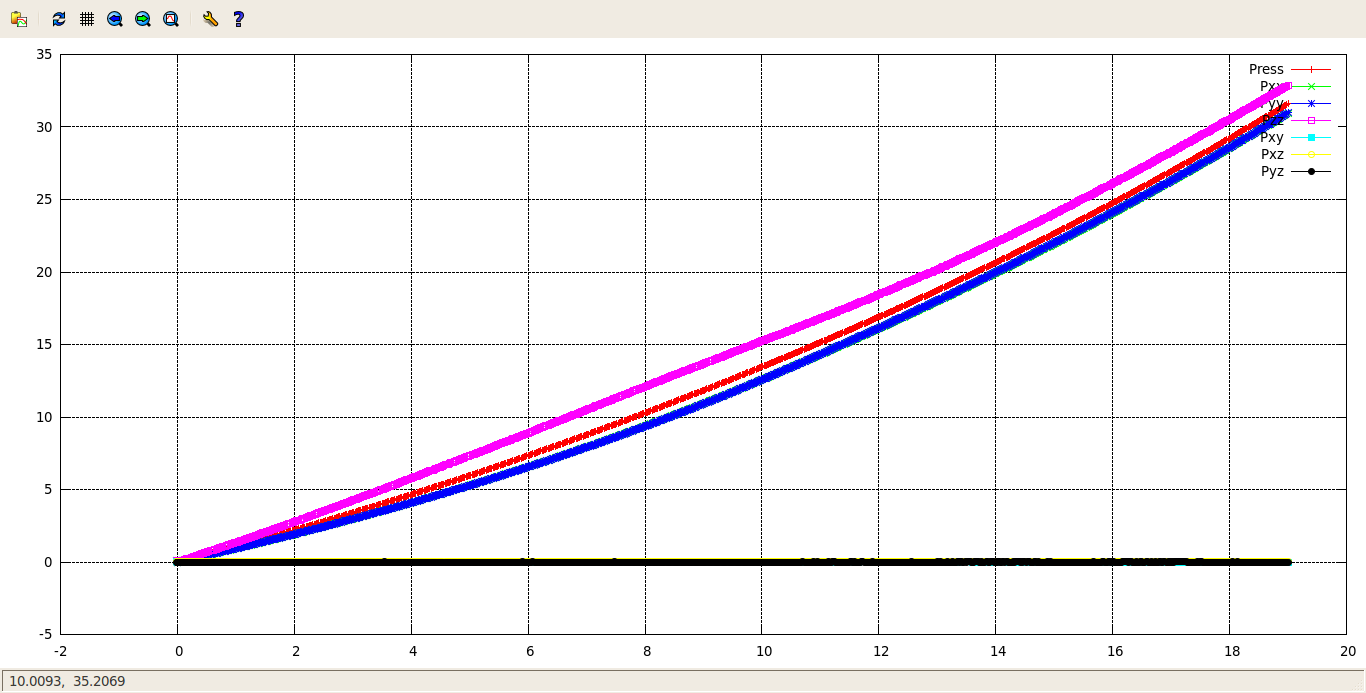
\includegraphics[width=8cm]{Figures/300-Tensiones-deformacion.png}
\caption{300K. Presiones vs strain}
\end{figure}

\begin{figure}[H]
\centering
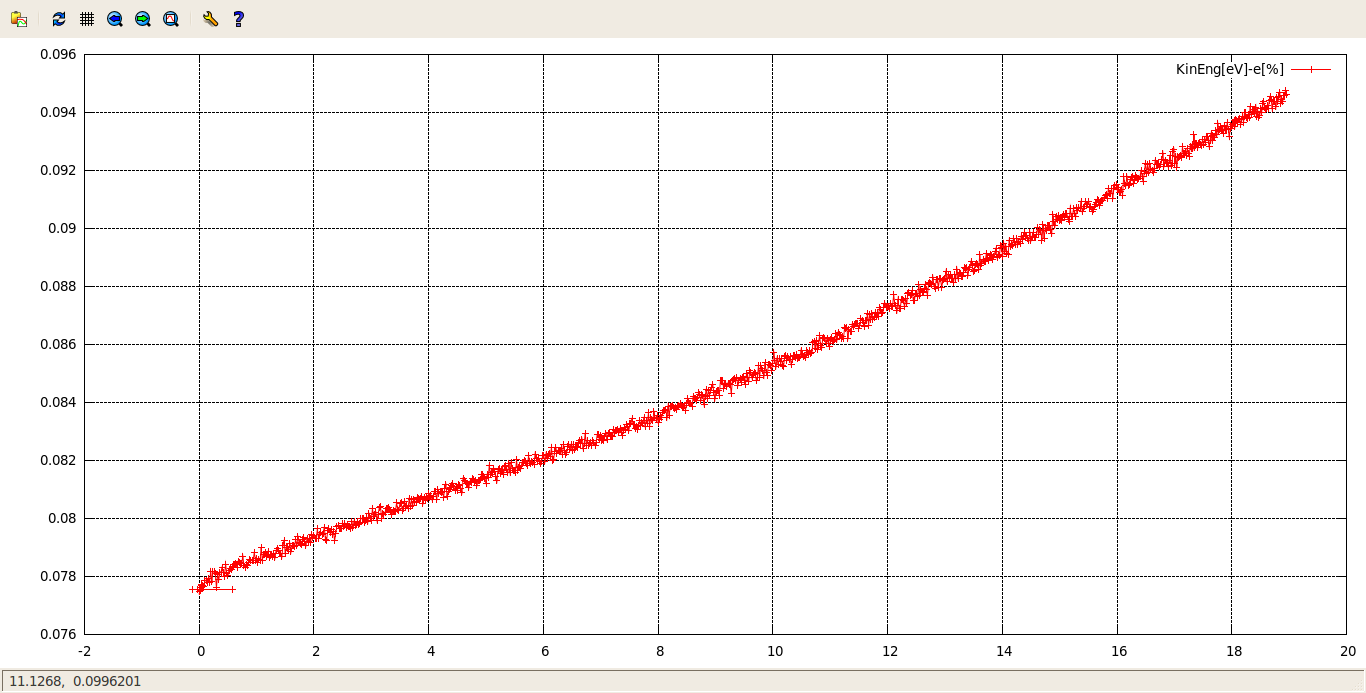
\includegraphics[width=8cm]{Figures/600-KinEng-deformacion.png}
\caption{600K. Energia cinetica vs strain}
\end{figure}

\begin{figure}[H]
\centering
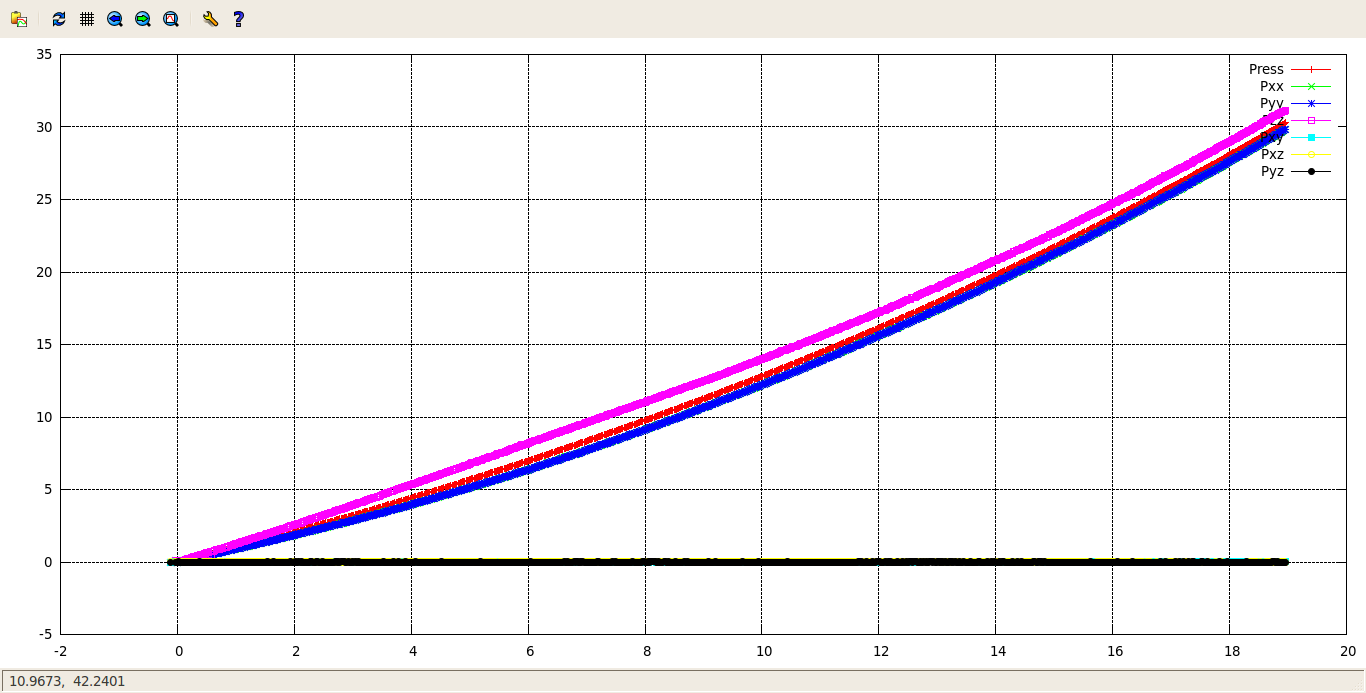
\includegraphics[width=8cm]{Figures/600-Tensiones-deformacion.png}
\caption{600K. Presiones vs strain}
\end{figure}

\begin{figure}[H]
\centering
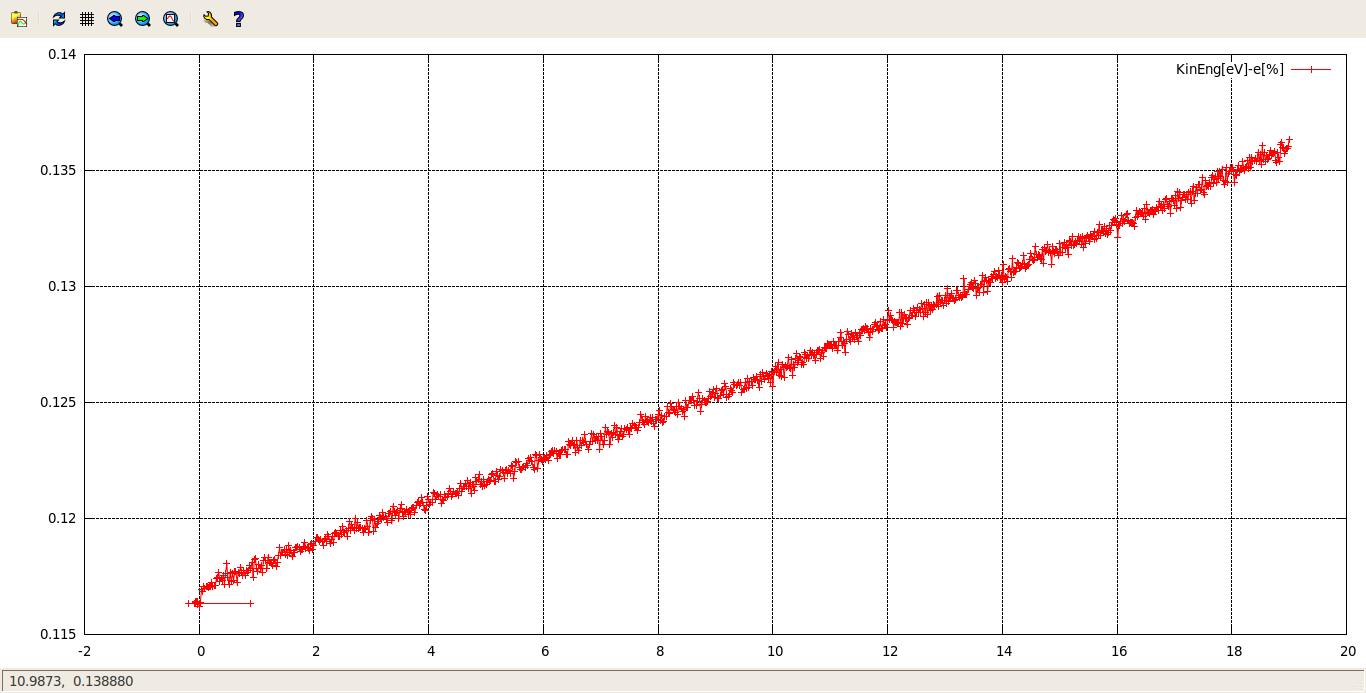
\includegraphics[width=8cm]{Figures/900-KinEng-deformacion.png}
\caption{900K. Energia cinetica vs strain}
\end{figure}

\begin{figure}[H]
\centering
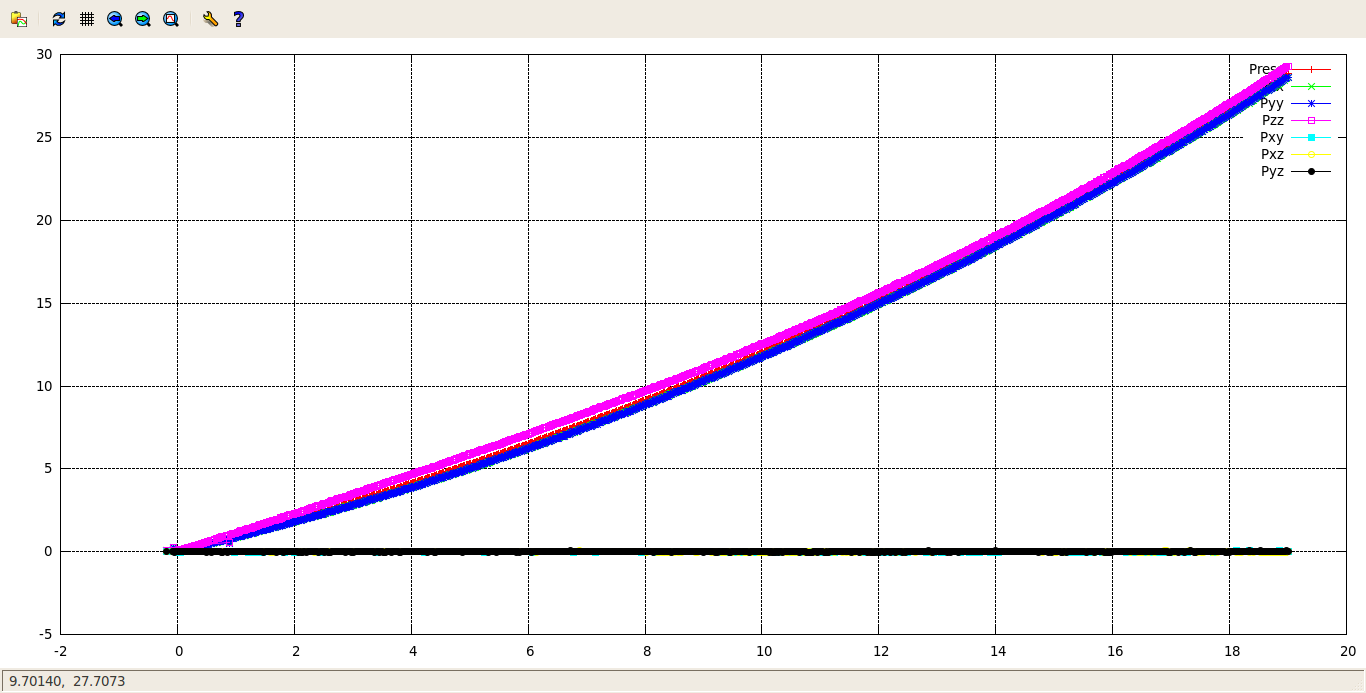
\includegraphics[width=8cm]{Figures/900-Tensiones-deformacion.png}
\caption{900K. Presiones vs strain}
\end{figure}

%
%	Traccion
%

\subsection{Traccion}

\begin{figure}[H]
\centering
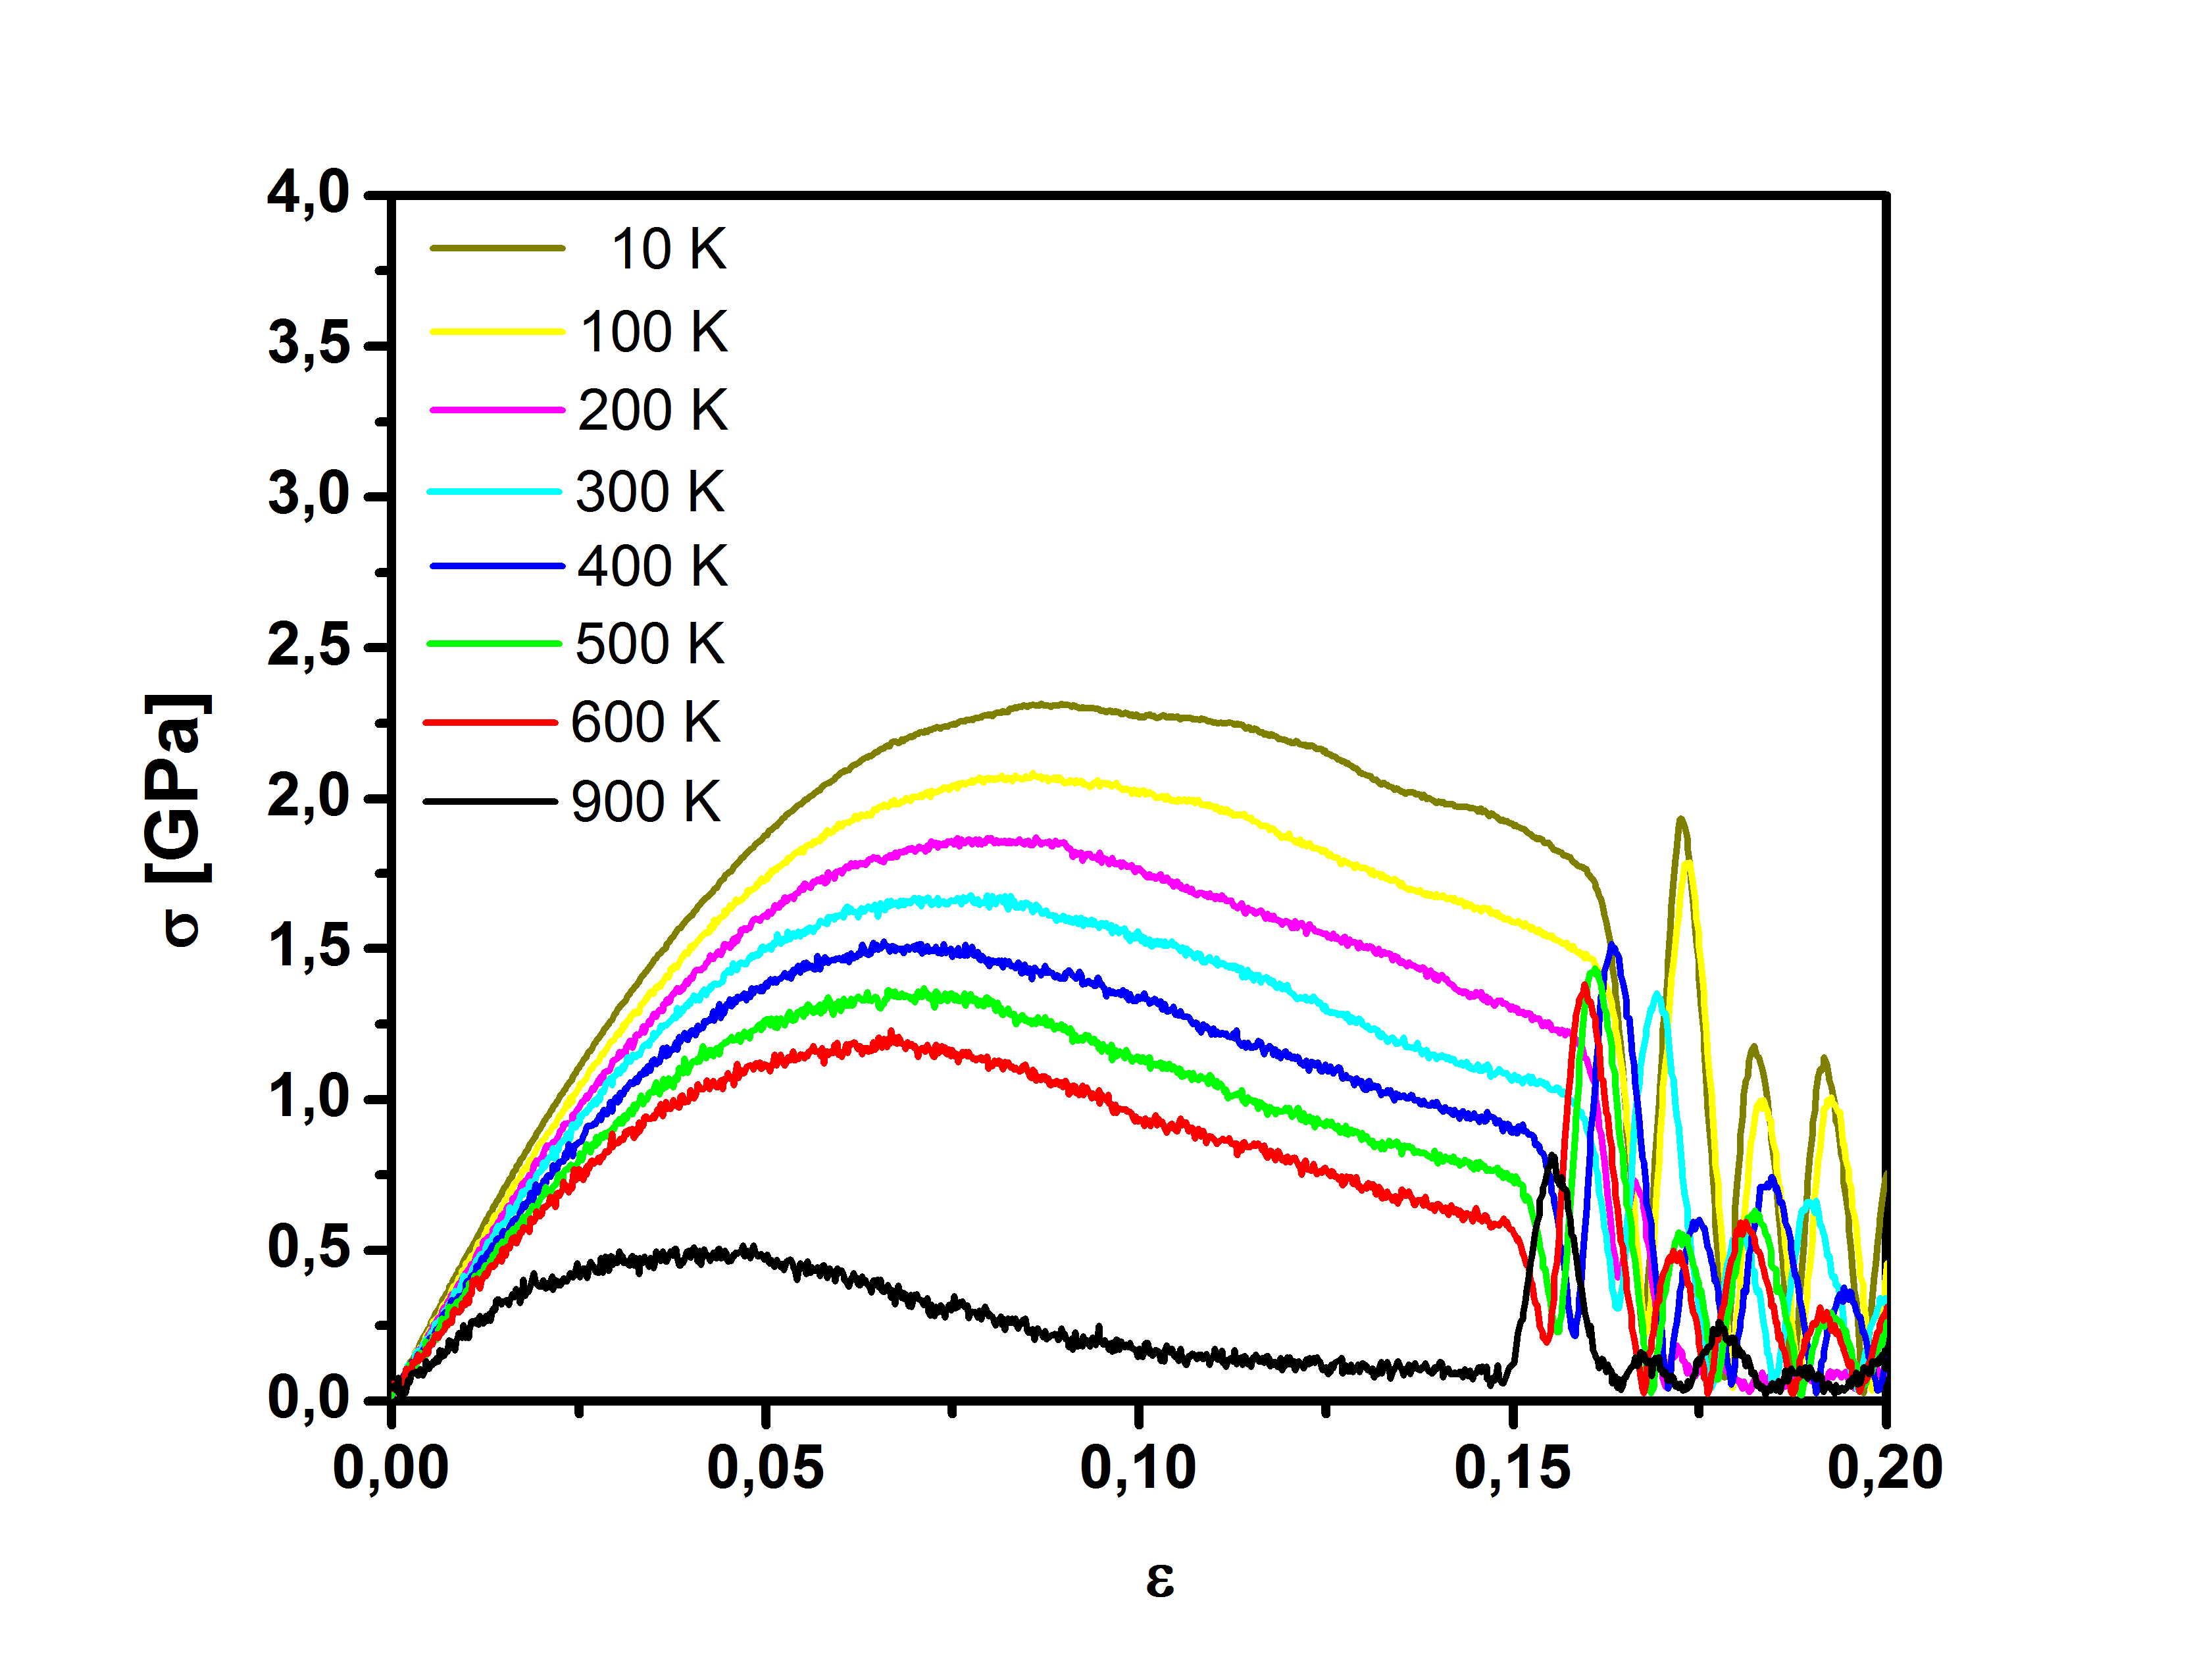
\includegraphics[width=8cm]{Figures/stress_strain_TEN.png}
\caption{Von Mises vs. strain}
\end{figure}

\begin{figure}[H]
\centering
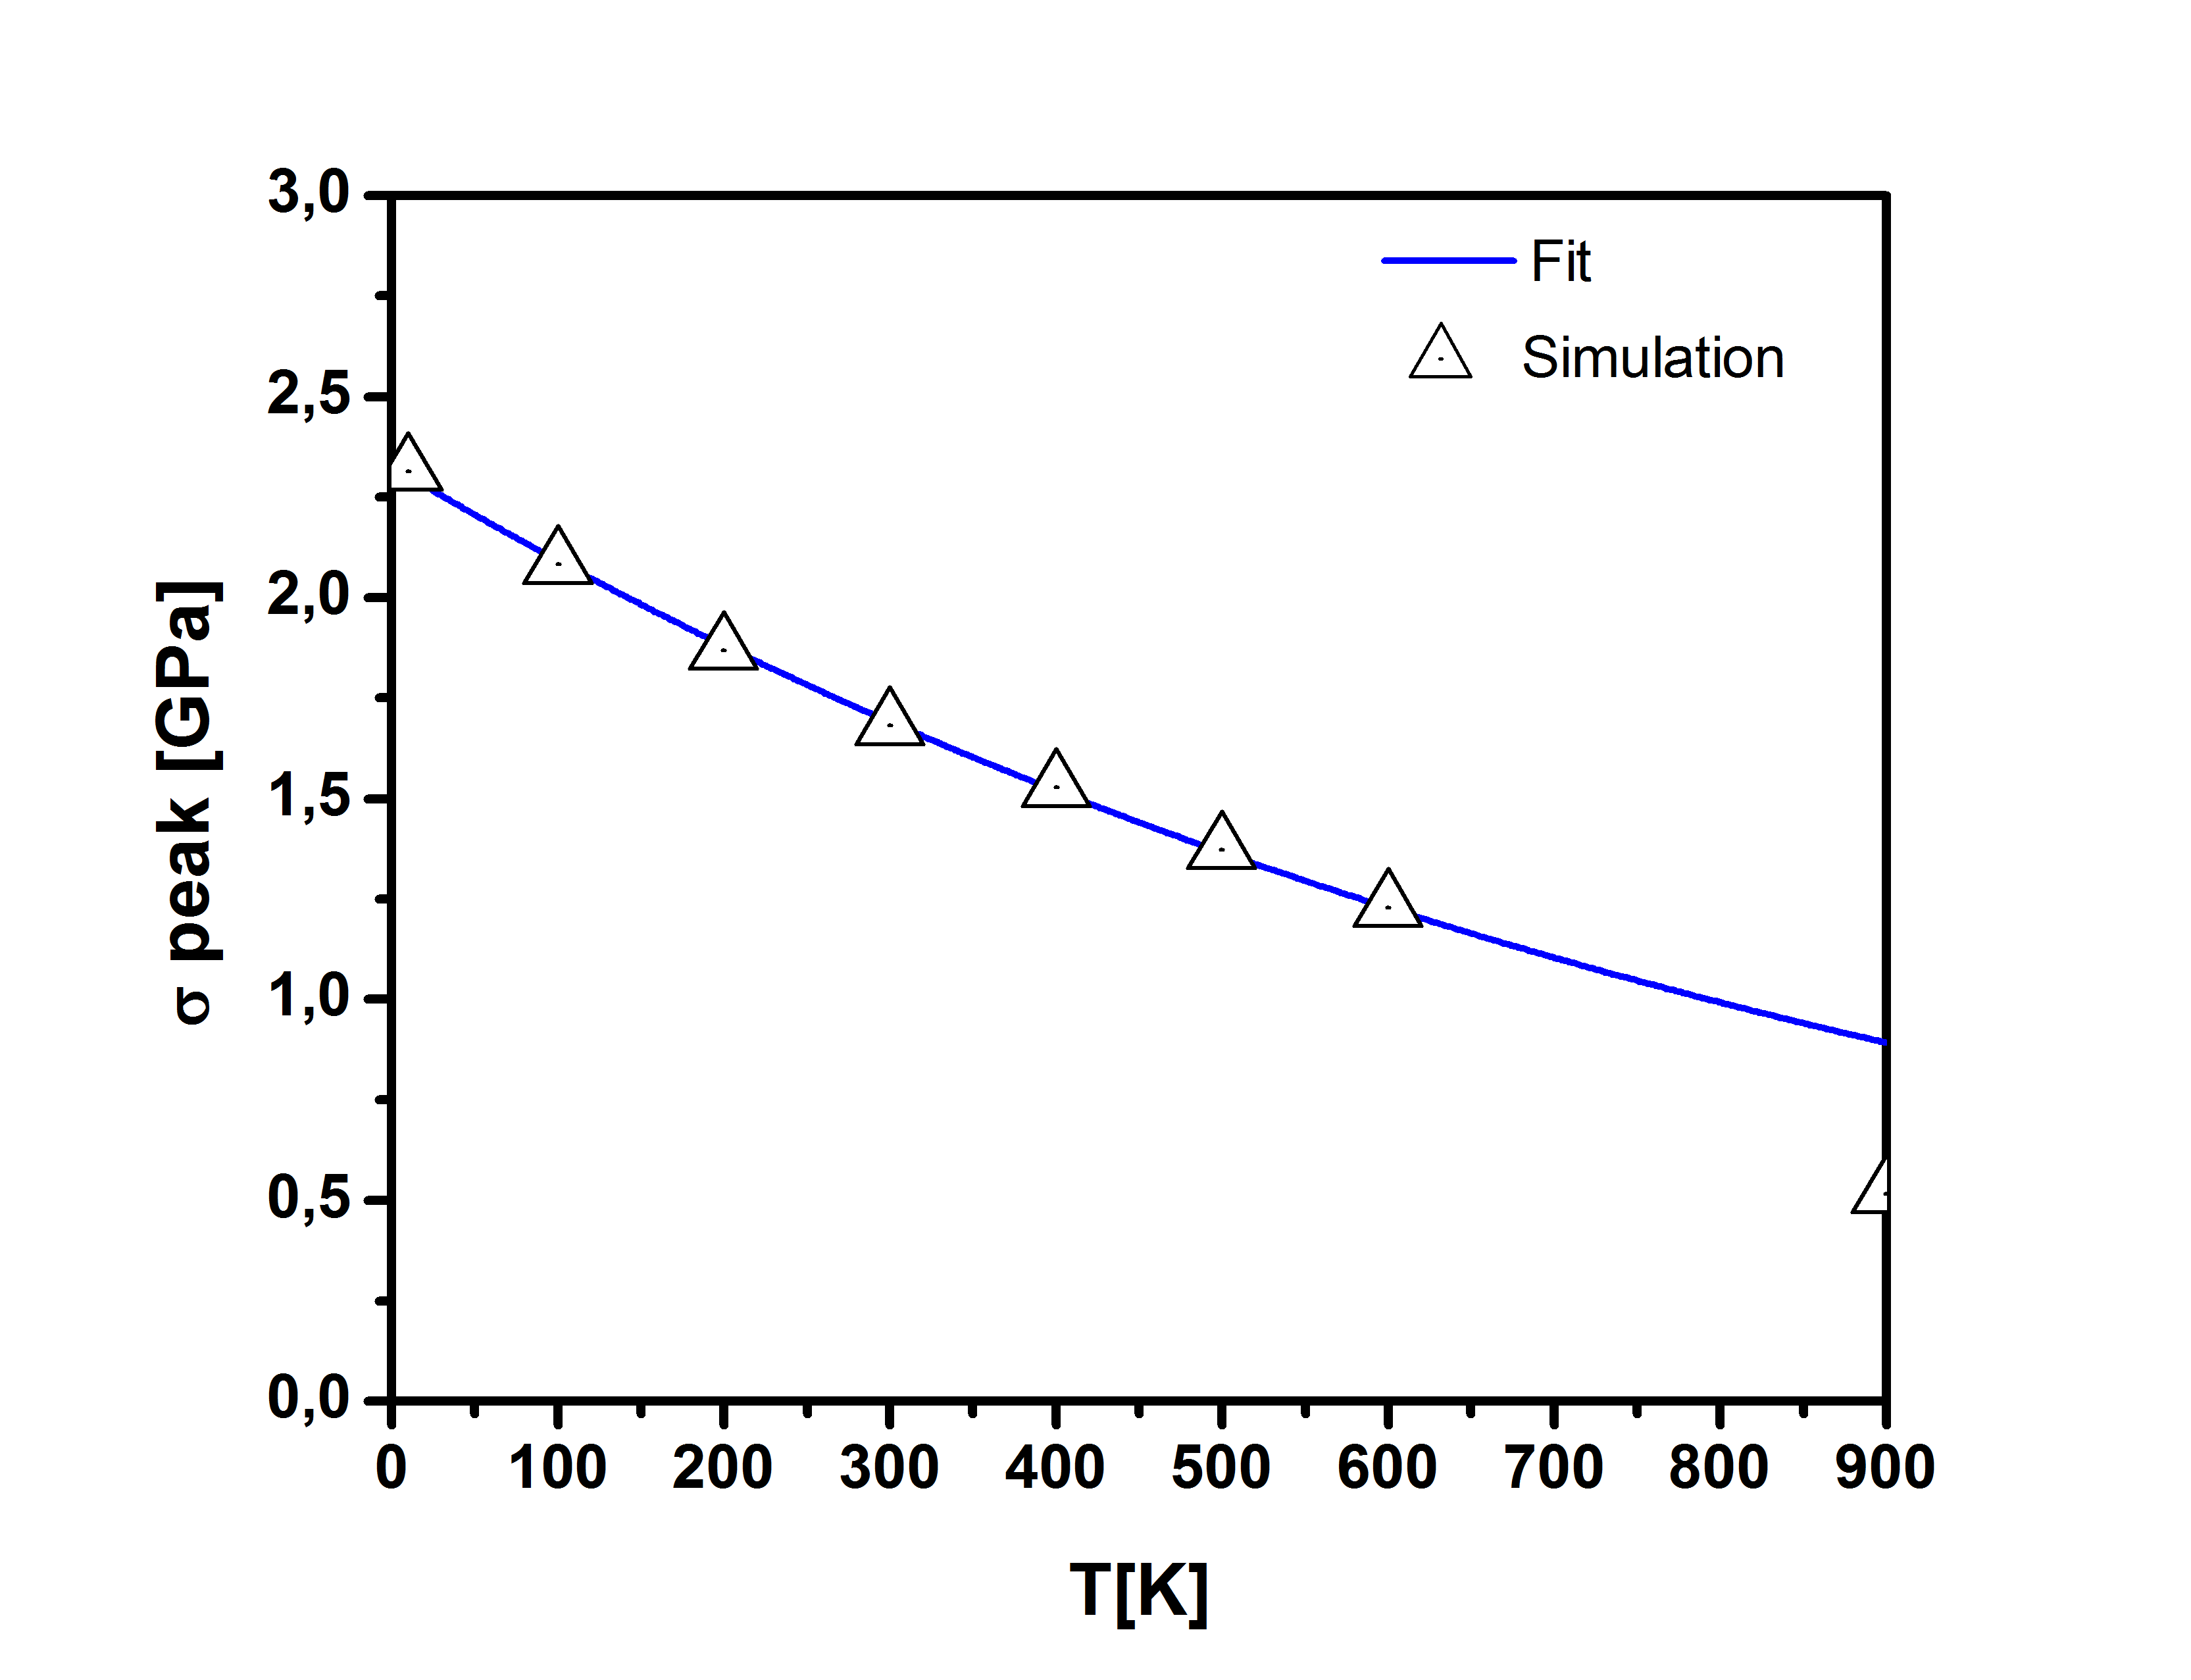
\includegraphics[width=8cm]{Figures/peakstress_T_TEN.png}
\caption{Von Mises maximo vs. Temperatura}
\end{figure}

\begin{figure}[H]
\centering
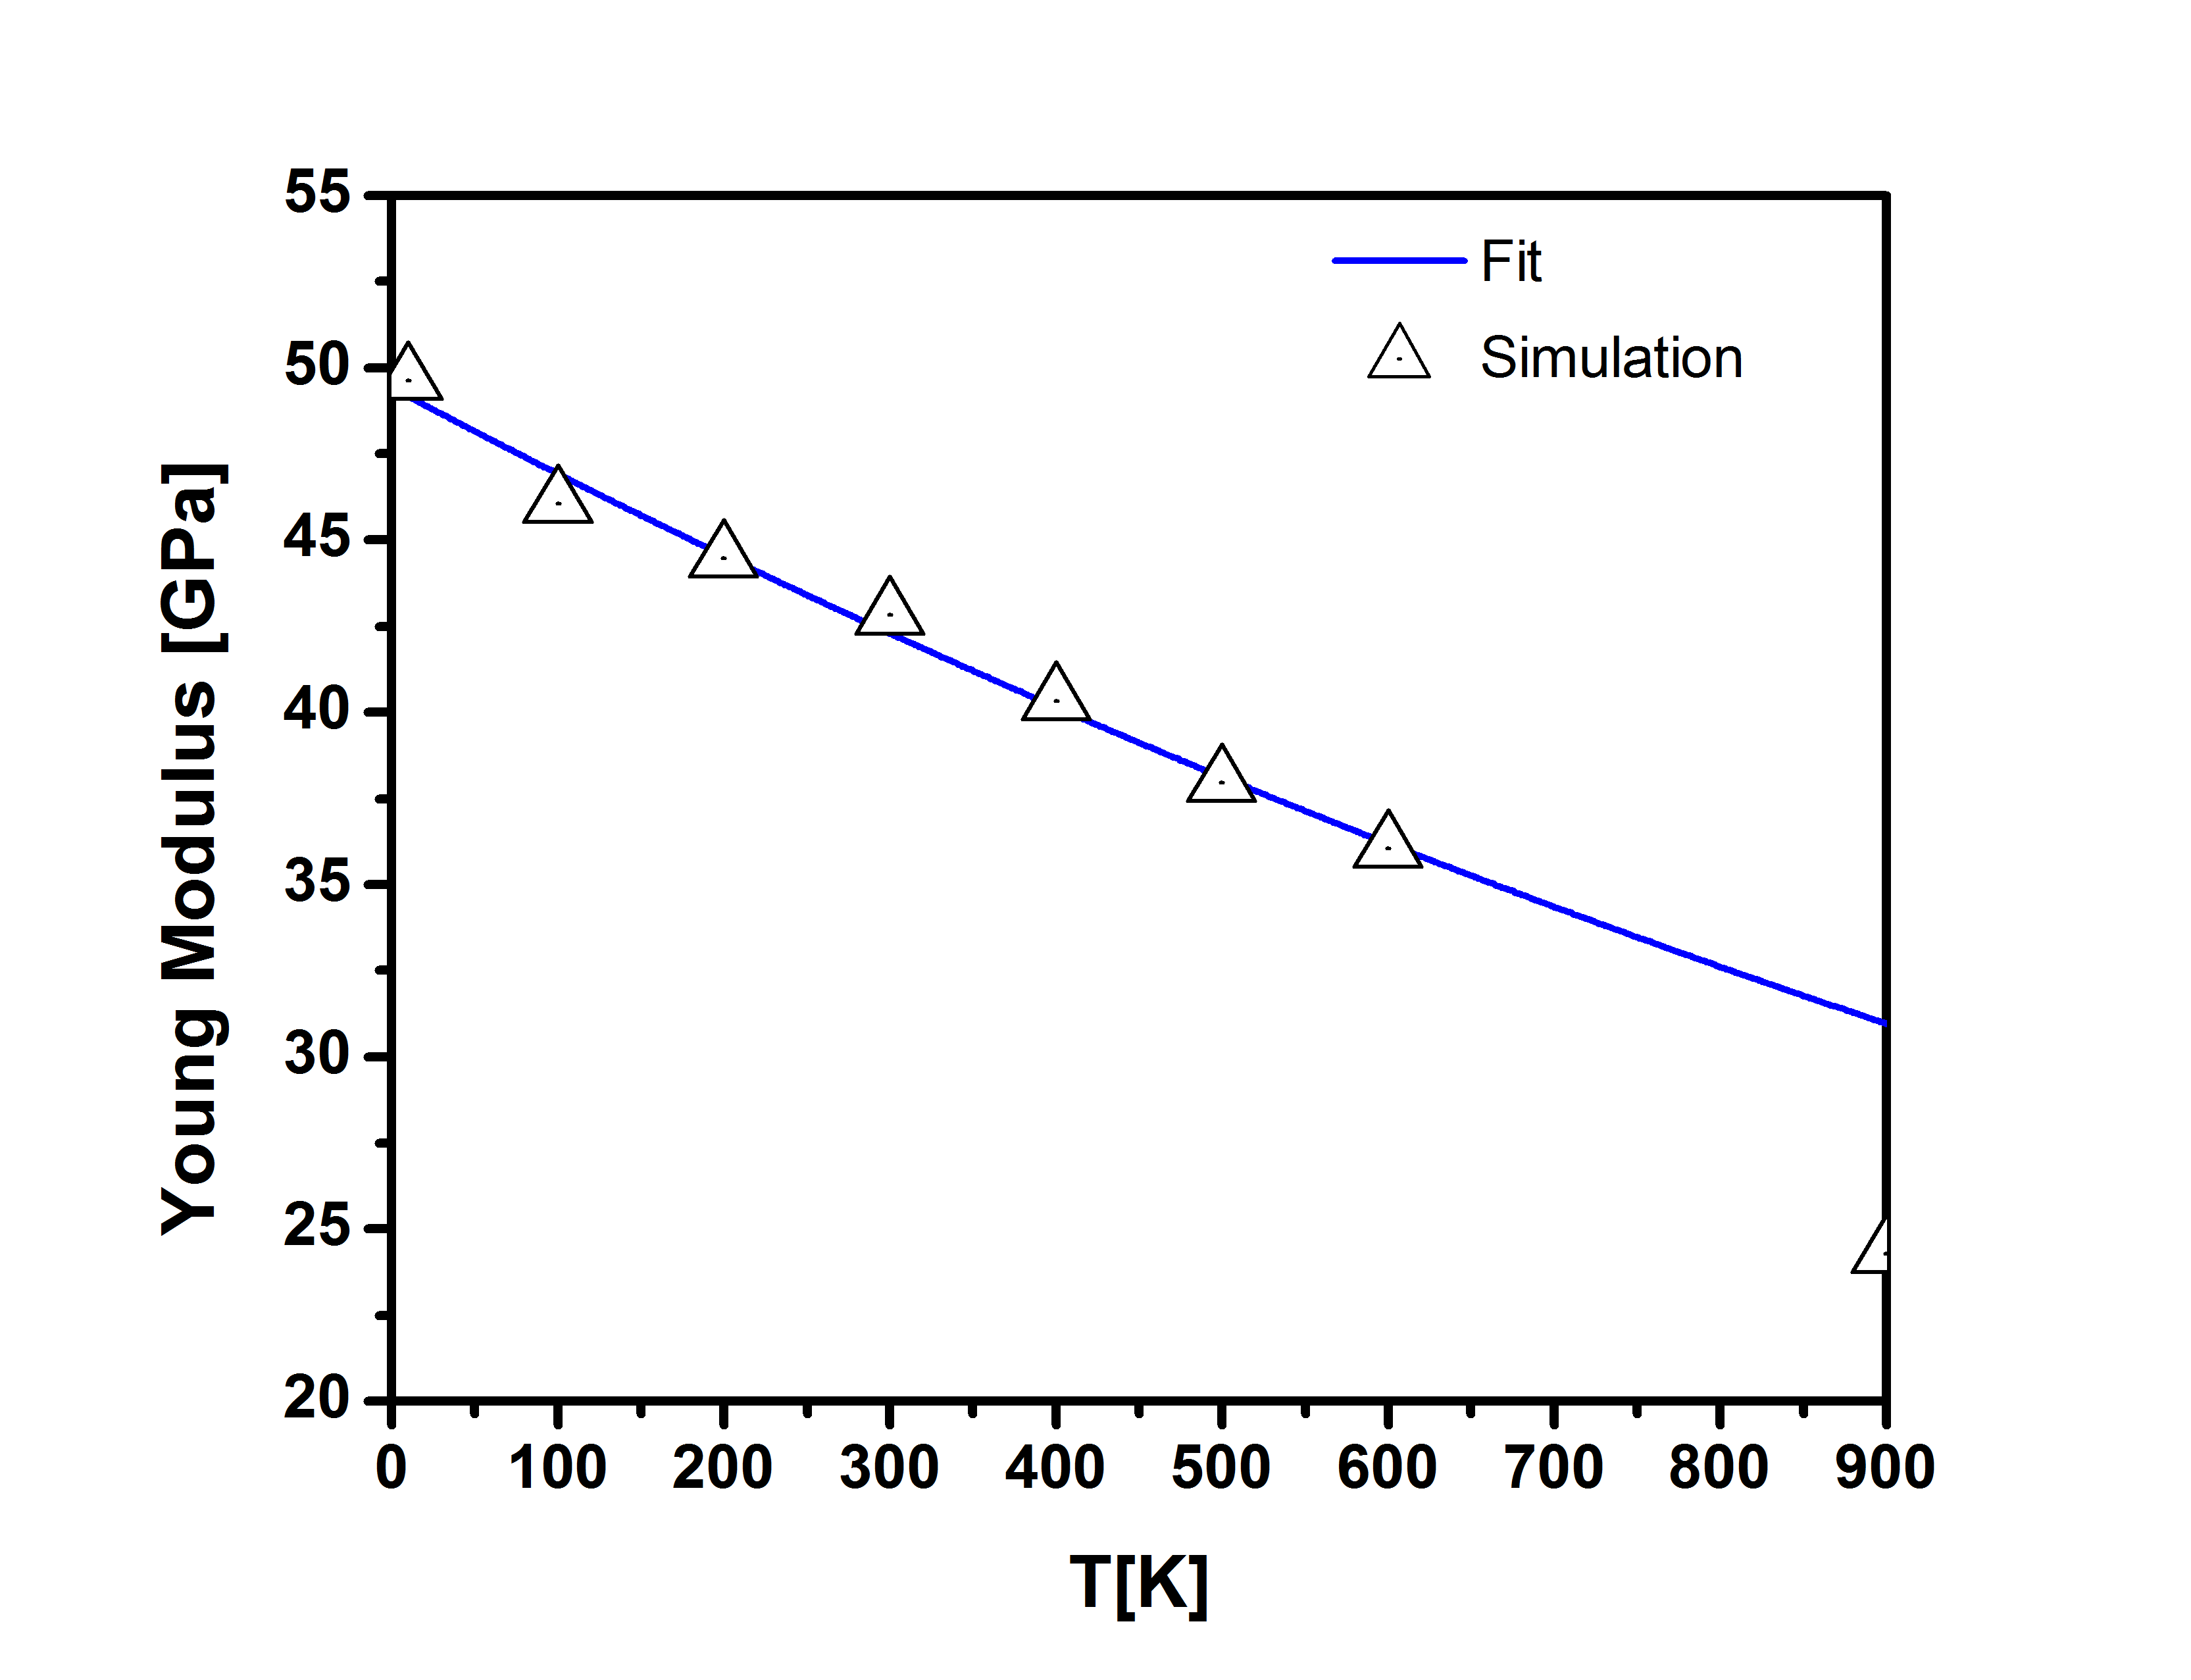
\includegraphics[width=8cm]{Figures/young_T_TEN.png}
\caption{Modulo Young vs. Temperatura}
\end{figure}

\begin{figure}[H]
\centering
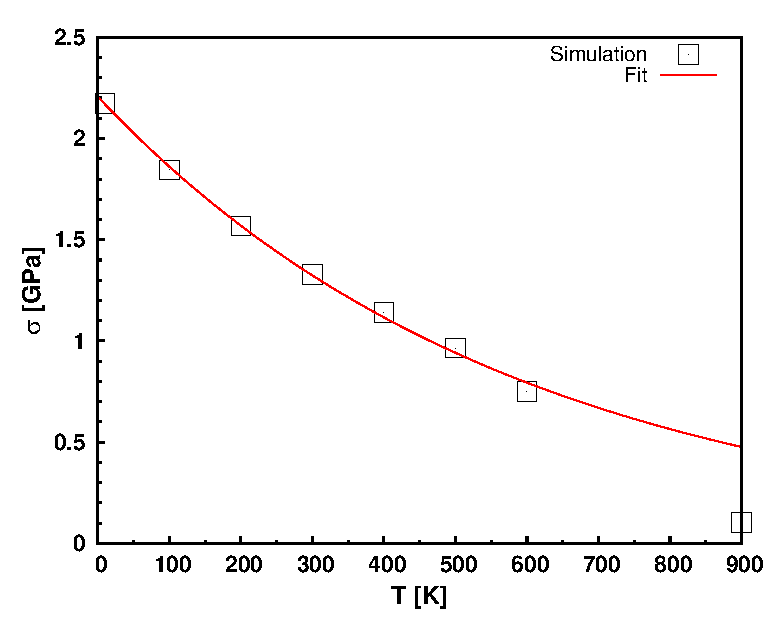
\includegraphics[width=8cm]{Figures/12stress_T_TENS.eps}
\caption{Von Mises a strain 12\% vs. Temperatura}
\end{figure}

\begin{figure}[H]
\centering
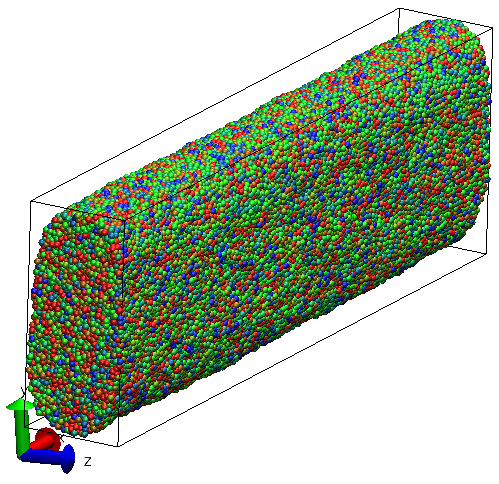
\includegraphics[width=8cm]{Figures/900libresTen.png}
\caption{Muestra a 300K cond. de frontera libres strain 20\%}
\end{figure}

\begin{figure}[H]
\centering
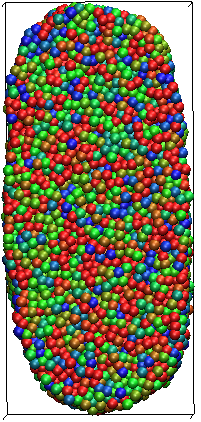
\includegraphics[width=2cm]{Figures/crossa.png}
\caption{Seccion transversal (cond. frontera libres) en el extremo de la muestra}
\end{figure}

\begin{figure}[H]
\centering
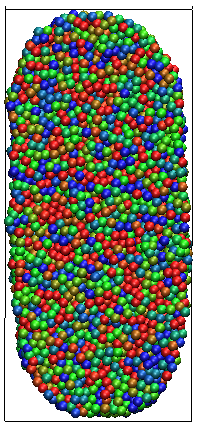
\includegraphics[width=2cm]{Figures/crossb.png}
\caption{Seccion transversal (cond. frontera libres) en el centro de la muestra}
\end{figure}

\begin{figure}[H]
\centering
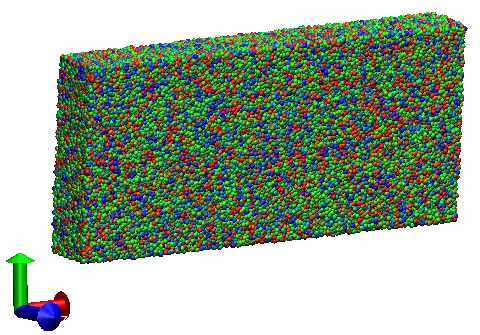
\includegraphics[width=8cm]{Figures/All_300K_6pstrain_sacale100-280_Trac.png}
\caption{Muestra a 300K cond. de frontera periodicas, 6\% strain, escala de colores 100-280 GPa}
\end{figure}

\begin{figure}[H]
\centering
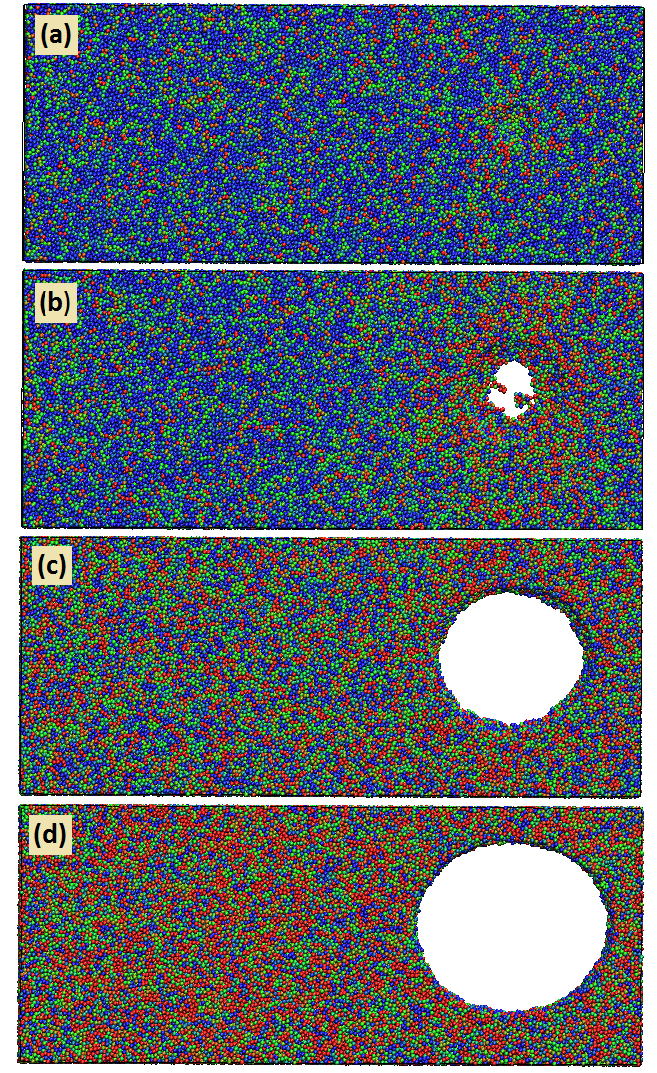
\includegraphics[width=8cm]{Figures/void_sequence.png}
\caption{Secuencia de formacion de void a 900K (strains 13.8, 14.2, 14.6, 15)}
\end{figure}

\begin{figure}[H]
\centering
\includegraphics[width=8cm]{Figures/VoidNucleationStrain_Vs_Temp_TENSION.png}
\caption{Strains de nucleacion de void vs. temperatura}
\end{figure}

\begin{figure}[H]
\centering
\includegraphics[width=8cm]{Figures/VoidNucleationStress_Vs_Temp_TENSION.png}
\caption{Stress de nucleacion de void vs. temperatura}
\end{figure}

\begin{figure}[H]
\centering
\includegraphics[width=8cm]{Figures/Tens_Polyedra_10K.jpeg}
\caption{Polyedros de voronoi vs. strain para 10K}
\end{figure}

\begin{figure}[H]
\centering
\includegraphics[width=8cm]{Figures/Polyedra_Vs_Strain_100K_TEN.png}
\caption{Num polyedros de voronoi vs. strain, a 100K}
\end{figure}

\begin{figure}[H]
\centering
\includegraphics[width=8cm]{Figures/Tens_Polyedra_200K.jpeg}
\caption{Polyedros de voronoi vs. strain para 200K}
\end{figure}

\begin{figure}[H]
\centering
\includegraphics[width=8cm]{Figures/Tens_Polyedra_300K.jpeg}
\caption{Polyedros de voronoi vs. strain para 300K}
\end{figure}

\begin{figure}[H]
\centering
\includegraphics[width=8cm]{Figures/Tens_Polyedra_400K.jpeg}
\caption{Polyedros de voronoi vs. strain para 400K}
\end{figure}

\begin{figure}[H]
\centering
\includegraphics[width=8cm]{Figures/Tens_Polyedra_500K.jpeg}
\caption{Polyedros de voronoi vs. strain para 500K}
\end{figure}

\begin{figure}[H]
\centering
\includegraphics[width=8cm]{Figures/Tens_Polyedra_600K.jpeg}
\caption{Polyedros de voronoi vs. strain para 600K}
\end{figure}

\begin{figure}[H]
\centering
\includegraphics[width=8cm]{Figures/Tens_Polyedra_900K.jpeg}
\caption{Polyedros de voronoi vs. strain para 900K}
\end{figure}

\begin{figure}[H]
\centering
\includegraphics[width=8cm]{Figures/Tension_Voro_Temp_5.jpeg}
\caption{Num polyedros de voronoi vs. temperatura, a strain 5\%}
\end{figure}

\begin{figure}[H]
\centering
\includegraphics[width=8cm]{Figures/poly_T_14strain_TEN.png}
\caption{Num polyedros de voronoi vs. temperatura, a strain 14\%}
\end{figure}

\begin{figure}[H]
\centering
\includegraphics[width=8cm]{Figures/type1_TEN.png}
\caption{polyedros de voronoi tipo 1 vs. strain}
\end{figure}

\begin{figure}[H]
\centering
\includegraphics[width=8cm]{Figures/type3_TEN.png}
\caption{polyedros de voronoi tipo 3 vs. strain}
\end{figure}

\begin{figure}[H]
\centering
\includegraphics[width=8cm]{Figures/TRAC_Vol_Step_A.png}
\caption{volumen promedio de voronoi cells (parte 1/2, temperatura desconocida)}
\end{figure}

\begin{figure}[H]
\centering
\includegraphics[width=8cm]{Figures/TRAC_Vol_Step_B.png}
\caption{volumen promedio de voronoi cells (parte 2/2, temperatura desconocida)}
\end{figure}

\begin{figure}[H]
\centering
\includegraphics[width=8cm]{Figures/TRAC_Num_Step_B.png}
\caption{numero celdas de voronoi (parte 1/4, temperatura desconocida)}
\end{figure}

\begin{figure}[H]
\centering
\includegraphics[width=8cm]{Figures/TRAC_Num_Step_C.png}
\caption{numero celdas de voronoi (parte 2/4, temperatura desconocida)}
\end{figure}

\begin{figure}[H]
\centering
\includegraphics[width=8cm]{Figures/TRAC_Num_Step_D.png}
\caption{numero celdas de voronoi (parte 3/4, temperatura desconocida)}
\end{figure}

\begin{figure}[H]
\centering
\includegraphics[width=8cm]{Figures/TRAC_Num_Step_E.png}
\caption{numero celdas de voronoi (parte 4/4, temperatura desconocida)}
\end{figure}

\begin{figure}[H]
\centering
\includegraphics[width=8cm]{Figures/600K_KinEnergy.png}
\caption{600K. Energia cinetica vs strain}
\end{figure}

\begin{figure}[H]
\centering
\includegraphics[width=8cm]{Figures/600K_PotEnergy.png}
\caption{600K. Energia potencial vs strain}
\end{figure}

\begin{figure}[H]
\centering
\includegraphics[width=8cm]{Figures/600K_PressVonMises.png}
\caption{600K. Presion von Mises vs strain}
\end{figure}

\begin{figure}[H]
\centering
\includegraphics[width=8cm]{Figures/600K_Temp.png}
\caption{600K. Temperatura vs strain}
\end{figure}

\begin{figure}[H]
\centering
\includegraphics[width=8cm]{Figures/600K_TensorPress.png}
\caption{600K. Presiones vs strain}
\end{figure}

\begin{figure}[H]
\centering
\includegraphics[width=8cm]{Figures/900K_KinEnergy.png}
\caption{900K. Energia cinetica vs strain}
\end{figure}

\begin{figure}[H]
\centering
\includegraphics[width=8cm]{Figures/900K_PotEnergy.png}
\caption{900K. Energia potencial vs strain}
\end{figure}

\begin{figure}[H]
\centering
\includegraphics[width=8cm]{Figures/900K_PressVonMises.png}
\caption{900K. Presion von Mises vs strain}
\end{figure}

\begin{figure}[H]
\centering
\includegraphics[width=8cm]{Figures/900K_Temp.png}
\caption{900K. Temperatura vs strain}
\end{figure}

\begin{figure}[H]
\centering
\includegraphics[width=8cm]{Figures/900K_TensorPress.png}
\caption{900K. Presiones vs strain}
\end{figure}

%
%	Ambas
%

\subsection{Comparacion}

\begin{figure}[H]
\centering
\includegraphics[width=8cm]{Figures/peakstress_T_BOTH.eps}
\caption{Von Mises maximo vs. Temperatura}
\end{figure}

\begin{figure}[H]
\centering
\includegraphics[width=8cm]{Figures/young_T_both.eps}
\caption{Modulo Young vs. Temperatura}
\end{figure}

\begin{figure}[H]
\centering
\includegraphics[width=8cm]{Figures/defstress_T_BOTH.eps}
\caption{Von Mises a strains vs. Temperatura}
\end{figure}

\begin{figure}[H]
\centering
\includegraphics[width=8cm]{Figures/Fit2_Tercios.png}
\caption{Comparacion curva Johnsohn}
\end{figure}


\section{Porosidad}

\subsection{Paper}

\begin{figure}[H]
  \centering
  \includegraphics[width=10cm]{Figures/Porosidad/spheres.png}
  \caption{Imágen de las nanopartículas esféricas de material.}
\end{figure}

\begin{figure}[H]
  \centering
  \includegraphics[width=10cm]{Figures/Porosidad/spheres3.png}
  \caption{Sinterizado 13\%}
\end{figure}

\begin{figure}[H]
  \centering
  \begin{tabular}{c}
    \subfloat[Porosidad 13\%, sin deformación]{\includegraphics[width=8cm]{Figures/Porosidad/13_0strain.png}} \\
    \subfloat[Porosidad 13\%, deformación 5\%]{\includegraphics[width=8cm]{Figures/Porosidad/13_5strain_comp.png}}
    \subfloat[Porosidad 13\%, deformación 12\%]{\includegraphics[width=8cm]{Figures/Porosidad/13_12strain_comp.png}}\\
  \end{tabular}
  \caption{Coloreado de una sección de la muestra con
  porosidad 13\% según la deformación cortante. El coloreado fue hecho usando Ovito, el color azul siendo 0.1 o menor y el color rojo 0.3 o mayor.
  (a) Estado inicial de la muestra (b) 5\% deformación por compresión (c) 12\% deformación por compresión.}
\end{figure}

\begin{figure}[H]
  \centering
  \begin{tabular}{c}
    \subfloat[Porosidad 13\%, sin deformación]{\includegraphics[width=8cm]{Figures/Porosidad/13_0strain.png}} \\
    \subfloat[Porosidad 13\%, deformación 5\%]{\includegraphics[width=8cm]{Figures/Porosidad/13_6strain_tens.png}}
    \subfloat[Porosidad 13\%, deformación 12\%]{\includegraphics[width=8cm]{Figures/Porosidad/13_20strain_tens.png}}\\
  \end{tabular}
  \caption{Coloreado de una sección de la muestra con
  porosidad 13\% según la deformación cortante. El coloreado fue hecho usando Ovito, el color azul siendo 0.1 o menor y el color rojo 0.3 o
  mayor. (a) 6\% deformación por tracción (b) 20\% deformación por tracción.}
  \label{C5:fg:ss_tens_13}
\end{figure}

\subsection{Fuera paper}

\begin{figure}[H]
  \centering
  \begin{tabular}{c}
    \subfloat[Porosidad 3\%, sin deformación]{\includegraphics[width=8cm]{Figures/Porosidad/3_0strain_pores.png}} \\
    \subfloat[Porosidad 3\%, deformación 5\%]{\includegraphics[width=8cm]{Figures/Porosidad/3_5strain_comp.png}}
    \subfloat[Porosidad 3\%, deformación 12\%]{\includegraphics[width=8cm]{Figures/Porosidad/3_12strain_comp.png}}\\
  \end{tabular}
  \caption[Coloreado de una sección de la muestra con porosidad 3\% según la deformación cortante para compresión.]{Coloreado de una sección de la muestra con
  porosidad 3\% según la deformación cortante. El coloreado fue hecho usando Ovito, el color azul siendo 0.1 o menor y el color rojo 0.3 o mayor.
  (a) Estado inicial de la muestra (b) 5\% deformación por compresión (c) 12\% deformación por compresión.}
  \label{C5:fg:ss_comp_3}
\end{figure}

\begin{figure}[H]
  \centering
  \begin{tabular}{c}
    \subfloat[Porosidad 6\%, sin deformación]{\includegraphics[width=8cm]{Figures/Porosidad/6_0strain_pores.png}} \\
    \subfloat[Porosidad 6\%, deformación 5\%]{\includegraphics[width=8cm]{Figures/Porosidad/6_5strain_comp.png}}
    \subfloat[Porosidad 6\%, deformación 12\%]{\includegraphics[width=8cm]{Figures/Porosidad/6_12strain_comp.png}}\\
  \end{tabular}
  \caption[Coloreado de una sección de la muestra con porosidad 6\% según la deformación cortante para compresión.]{Coloreado de una sección de la muestra con
  porosidad 6\% según la deformación cortante. El coloreado fue hecho usando Ovito, el color azul siendo 0.1 o menor y el color rojo 0.3 o mayor.
  (a) Estado inicial de la muestra (b) 5\% deformación por compresión (c) 12\% deformación por compresión.}
  \label{C5:fg:ss_comp_6}
\end{figure}

\begin{figure}[H]
  \centering
  \begin{tabular}{c}
    \subfloat[Porosidad 13\%, sin deformación]{\includegraphics[width=8cm]{Figures/Porosidad/13_0strain.png}} \\
    \subfloat[Porosidad 13\%, deformación 5\%]{\includegraphics[width=8cm]{Figures/Porosidad/13_5strain_comp.png}}
    \subfloat[Porosidad 13\%, deformación 12\%]{\includegraphics[width=8cm]{Figures/Porosidad/13_12strain_comp.png}}\\
  \end{tabular}
  \caption[Coloreado de una sección de la muestra con porosidad 13\% según la deformación cortante para compresión.]{Coloreado de una sección de la muestra con
  porosidad 13\% según la deformación cortante. El coloreado fue hecho usando Ovito, el color azul siendo 0.1 o menor y el color rojo 0.3 o mayor.
  (a) Estado inicial de la muestra (b) 5\% deformación por compresión (c) 12\% deformación por compresión.}
  \label{C5:fg:ss_comp_13}
\end{figure}

\begin{figure}[H]
  \centering
  \begin{tabular}{c}
    \subfloat[Porosidad 3\%, sin deformación]{\includegraphics[width=8cm]{Figures/Porosidad/3_0strain_pores_tens.png}}
    \subfloat[Porosidad 3\%, deformación 5\%]{\includegraphics[width=8cm]{Figures/Porosidad/3_5strain_tens.png}} \\
    \subfloat[Porosidad 3\%, deformación 12\%]{\includegraphics[width=8cm]{Figures/Porosidad/3_12strain_tens.png}}
    \subfloat[Porosidad 3\%, deformación 20\%]{\includegraphics[width=8cm]{Figures/Porosidad/3_20strain_tens.png}}
  \end{tabular}
  \caption[Coloreado de una sección de la muestra con porosidad 3\% según la deformación cortante para tracción.]{Coloreado de una sección de la muestra con
  porosidad 3\% según la deformación cortante. El coloreado fue hecho usando Ovito, el color azul siendo 0.1 o menor y el color rojo 0.3 o
  mayor. (a) Estado inicial de la muestra. (b) 5\% deformación por tracción (c) 12\% deformación por tracción. (d) 20\% deformación por tracción.}
  \label{C5:fg:ss_tens_3}
\end{figure}

\clearpage

\begin{figure}[H]
  \centering
  \begin{tabular}{c}
    \subfloat[Porosidad 6\%, sin deformación]{\includegraphics[width=8cm]{Figures/Porosidad/6_0strain_pores_tens.png}} 
    \subfloat[Porosidad 6\%, deformación 5\%]{\includegraphics[width=8cm]{Figures/Porosidad/6_5strain_tens.png}} \\
    \subfloat[Porosidad 6\%, deformación 12\%]{\includegraphics[width=8cm]{Figures/Porosidad/6_12strain_tens.png}}
    \subfloat[Porosidad 6\%, deformación 20\%]{\includegraphics[width=8cm]{Figures/Porosidad/6_20strain_tens.png}}
  \end{tabular}
  \caption[Coloreado de una sección de la muestra con porosidad 6\% según la deformación cortante para tracción.]{Coloreado de una sección de la muestra con
  porosidad 6\% según la deformación cortante. El coloreado fue hecho usando Ovito, el color azul siendo 0.1 o menor y el color rojo 0.3 o
  mayor. (a) Estado inicial de la muestra. (b) 5\% deformación por tracción (c) 12\% deformación por tracción. (d) 20\% deformación por tracción.}
  \label{C5:fg:ss_tens_6}
\end{figure}

\clearpage

\begin{figure}[H]
  \centering
  \begin{tabular}{c}
    \subfloat[Porosidad 13\%, sin deformación]{\includegraphics[width=8cm]{Figures/Porosidad/13_0strain_pores_tens.png}} 
    \subfloat[Porosidad 13\%, deformación 5\%]{\includegraphics[width=8cm]{Figures/Porosidad/13_5strain_tens.png}}\\
    \subfloat[Porosidad 13\%, deformación 12\%]{\includegraphics[width=8cm]{Figures/Porosidad/13_12strain_tens.png}}
    \subfloat[Porosidad 13\%, deformación 20\%]{\includegraphics[width=8cm]{Figures/Porosidad/13_20strain_tens2.png}}
  \end{tabular}
  \caption[Coloreado de una sección de la muestra con porosidad 13\% según la deformación cortante para tracción.]{Coloreado de una sección de la muestra con
  porosidad 13\% según la deformación cortante. El coloreado fue hecho usando Ovito, el color azul siendo 0.1 o menor y el color rojo 0.3 o
  mayor. (a) Estado inicial de la muestra. (b) 5\% deformación por tracción (c) 12\% deformación por tracción. (d) 20\% deformación por tracción.}
  \label{C5:fg:ss_tens_13}
\end{figure}

\begin{figure}[H]
\centering
\includegraphics[width=8cm]{Figures/Porosidad/5_0strain.png}
\caption{Porosidad 3\%. 0 strain}
\end{figure}

\begin{figure}[H]
\centering
\includegraphics[width=8cm]{Figures/Porosidad/5_0strain_color.png}
\caption{Porosidad 3\%. 0 strain}
\end{figure}

\begin{figure}[H]
\centering
\includegraphics[width=8cm]{Figures/Porosidad/5_2strain_color.png}
\caption{Porosidad 3\%. 2\% strain}
\end{figure}

\begin{figure}[H]
\centering
\includegraphics[width=8cm]{Figures/Porosidad/5_14strain_color.png}
\caption{Porosidad 3\%. 14\% strain}
\end{figure}

\begin{figure}[H]
\centering
\includegraphics[width=8cm]{Figures/Porosidad/5_15strain_color.png}
\caption{Porosidad 3\%. 15\% strain}
\end{figure}

\begin{figure}[H]
\centering
\includegraphics[width=8cm]{Figures/Porosidad/9_0strain.png}
\caption{Porosidad 6\%. 0 strain}
\end{figure}

\begin{figure}[H]
\centering
\includegraphics[width=8cm]{Figures/Porosidad/9_0strain_color.png}
\caption{Porosidad 6\%. 0 strain}
\end{figure}

\begin{figure}[H]
\centering
\includegraphics[width=8cm]{Figures/Porosidad/9_2strain_color.png}
\caption{Porosidad 6\%. 2\% strain}
\end{figure}

\begin{figure}[H]
\centering
\includegraphics[width=8cm]{Figures/Porosidad/9_15strain_color.png}
\caption{Porosidad 6\%. 15\% strain}
\end{figure}

\begin{figure}[H]
\centering
\includegraphics[width=8cm]{Figures/Porosidad/18_0strain.png}
\caption{Porosidad 13\%. 0 strain}
\end{figure}

\begin{figure}[H]
\centering
\includegraphics[width=8cm]{Figures/Porosidad/18_0strain_color.png}
\caption{Porosidad 13\%. 0 strain}
\end{figure}

\begin{figure}[H]
\centering
\includegraphics[width=8cm]{Figures/Porosidad/18_2strain_color.png}
\caption{Porosidad 13\%. 2\% strain}
\end{figure}

\begin{figure}[H]
\centering
\includegraphics[width=8cm]{Figures/Porosidad/18_15strain_color.png}
\caption{Porosidad 13\%. 15\% strain}
\end{figure}

\begin{figure}[H]
\centering
\includegraphics[width=8cm]{Figures/Porosidad/18_20strain_color.png}
\caption{Porosidad 13\%. 20\% strain}
\end{figure}

\begin{figure}[H]
\centering
\includegraphics[width=8cm]{Figures/Porosidad/porosity_cu_strain.eps}
\caption{Polyedros de voronoi centrados en atomos de cobre vs strain. Compresion}
\end{figure}

\begin{figure}[H]
\centering
\includegraphics[width=8cm]{Figures/Porosidad/porosity_Pzz_strain_comp.eps}
\caption{Pzz vs. strain. Compresion.}
\end{figure}

\begin{figure}[H]
\centering
\includegraphics[width=8cm]{Figures/Porosidad/porosity_Pzz_strain_comp_dash.eps}
\caption{Pzz vs. strain. Compresion. La linea punteada indica donde SVF = 1}
\end{figure}

\begin{figure}[H]
\centering
\includegraphics[width=8cm]{Figures/Porosidad/porosity_Pzz_strain_tens.eps}
\caption{Pzz vs. strain. Traccion.}
\end{figure}

%\begin{figure}[H]
%\centering
%\includegraphics[width=8cm]{Figures/Porosidad/porosity_Pzz_strain_tens_dash.eps}
%\caption{Pzz vs. strain. Traccion.}
%\end{figure}

\begin{figure}[H]
\centering
\includegraphics[width=8cm]{Figures/Porosidad/porosity_stress_strain_comp.eps}
\caption{Stress VM vs strain. Compresion.}
\end{figure}

\begin{figure}[H]
\centering
\includegraphics[width=8cm]{Figures/Porosidad/porosity_stress_strain_comp_dash.eps}
\caption{Stress VM vs strain. Compresion. La linea punteada indica donde SVF = 1}
\end{figure}

\begin{figure}[H]
\centering
\includegraphics[width=8cm]{Figures/Porosidad/porosity_stress_strain_tens.eps}
\caption{Stress VM vs strain. Traccion.}
\end{figure}

%\begin{figure}[H]
%\centering
%\includegraphics[width=8cm]{Figures/Porosidad/porosity_stress_strain_tens_dash.eps}
%\caption{???}
%\end{figure}

\begin{figure}[H]
\centering
\includegraphics[width=8cm]{Figures/Porosidad/porosity_SVF_strain.eps}
\caption{Fraccion de volumen solido vs. strain}
\end{figure}

\begin{figure}[H]
\centering
\includegraphics[width=8cm]{Figures/Porosidad/porosity_SVF_strain_comp.eps}
\caption{Fraccion de volumen solido vs. strain. Compresion}
\end{figure}

\begin{figure}[H]
\centering
\includegraphics[width=8cm]{Figures/Porosidad/porosity_SVF_strain_comp_dash.eps}
\caption{Fraccion de volumen solido vs. strain. Compresion. La linea punteada marca cuando SVF = 1. Para 13\% porosidad vemos que hay cambios de pendiente al 0.01, 0.095 y 0.12 strain. Estos valores se corresponden con los puntos donde la curva temperatura-strain cambia de pendiente. Para 6\% porosidad hay cambio de pendiente a 0.005, 0.04 y 0.065 strain. El primer cambio de pendiente es tal vez poco significativo, ya que la resolución de la curva es justamente 0.005 strain. }
\end{figure}

%\begin{figure}[H]
%\centering
%\includegraphics[width=8cm]{Figures/Porosidad/porosity_SVF_strain_comp_dash2.eps}
%\caption{???}
%\end{figure}

\begin{figure}[H]
\centering
\includegraphics[width=8cm]{Figures/Porosidad/porosity_SVF_strain_tens.eps}
\caption{Fraccion de volumen solido vs. strain. Traccion}
\end{figure}

%\begin{figure}[H]
%\centering
%\includegraphics[width=8cm]{Figures/Porosidad/porosity_SVF_strain_tens_dash.eps}
%\caption{???}
%\end{figure}

%\begin{figure}[H]
%\centering
%\includegraphics[width=8cm]{Figures/Porosidad/porosity_SVF_strain_tens_dash2.eps}
%\caption{???}
%\end{figure}

\begin{figure}[H]
\centering
\includegraphics[width=8cm]{Figures/Porosidad/porosity_temp_strain_comp.eps}
\caption{Temperatura vs strain. Compresion}
\end{figure}

\begin{figure}[H]
\centering
\includegraphics[width=8cm]{Figures/Porosidad/porosity_temp_strain_comp_dash.eps}
\caption{Temperatura vs. strain. Compresion. La linea punteada indica cuando SVF = 1}
\end{figure}

\begin{figure}[H]
\centering
\includegraphics[width=8cm]{Figures/Porosidad/porosity_temp_strain_tens.eps}
\caption{Temperatura vs strain. Traccion}
\end{figure}

%\begin{figure}[H]
%\centering
%\includegraphics[width=8cm]{Figures/Porosidad/porosity_temp_strain_tens_dash.eps}
%\caption{???}
%\end{figure}

\begin{figure}[H]
\centering
\includegraphics[width=8cm]{Figures/Porosidad/porosity_tipe3_strain_comp.eps}
\caption{Polyedros de voronoi tipo 3 Compresion.}
\end{figure}

\begin{figure}[H]
\centering
\includegraphics[width=8cm]{Figures/Porosidad/porosity_tipe3_strain_tens.eps}
\caption{Polyedros de voronoi tipo 3. Traccion}
\end{figure}

\begin{figure}[H]
\centering
\includegraphics[width=8cm]{Figures/Porosidad/porosidad_STZObservation_3_0.png}
\caption{Porosidad 3\%. Surgimiento de STZ lejos de los poros. Strain 0. Atomos shear strain superior a 0.25. Compresion. Parte 1/3}
\end{figure}

\begin{figure}[H]
\centering
\includegraphics[width=8cm]{Figures/Porosidad/porosidad_STZObservation_3_0005.png}
\caption{Porosidad 3\%. Surgimiento de STZ lejos de los poros. Strain 0.005. Atomos shear strain superior a 0.25. Compresion. Parte 2/3}
\end{figure}

\begin{figure}[H]
\centering
\includegraphics[width=8cm]{Figures/Porosidad/porosidad_STZObservation_3_01.png}
\caption{Porosidad 3\%. Surgimiento de STZ lejos de los poros. Strain 0.1. Atomos shear strain superior a 0.25. Compresion. Parte 3/3}
\end{figure}

\begin{figure}[H]
\centering
\includegraphics[width=8cm]{Figures/Porosidad/porosidad_3_faceAS_0_02.png}
\caption{Porosidad 3\%. Cara de la muestra. Strain 0. Color coding con shear strain entre 0 y 0.2. Compresion. Parte 1/3}
\end{figure}

\begin{figure}[H]
\centering
\includegraphics[width=8cm]{Figures/Porosidad/porosidad_3_faceAS_0_02_0005.png}
\caption{Porosidad 3\%. Cara de la muestra. Strain 0.005. Color coding con shear strain entre 0 y 0.2. Compresion. Parte 2/3}
\end{figure}

\begin{figure}[H]
\centering
\includegraphics[width=8cm]{Figures/Porosidad/porosidad_3_faceAS_0_02_001.png}
\caption{Porosidad 3\%. Cara de la muestra. Strain 0.01. Color coding con shear strain entre 0 y 0.2. Compresion. Parte 3/3}
\end{figure}

\begin{figure}[H]
\centering
\includegraphics[width=8cm]{Figures/Porosidad/porosidad_6_shearstrain04_0.png}
\caption{Porosidad 6\%. Strain 0. Los átomos coloreados son aquellos con shear strain superior a 0.4. Los mayores valores de shear strain se dan alrededor de los poros. Incluso cuando los poros ya se han colapsado, la distribución de shear strain conserva la misma forma. Compresion. Parte 1/4}
\end{figure}

\begin{figure}[H]
\centering
\includegraphics[width=8cm]{Figures/Porosidad/porosidad_6_shearstrain04_006.png}
\caption{Porosidad 6\%. Strain 0.06. Los átomos coloreados son aquellos con shear strain superior a 0.4. Los mayores valores de shear strain se dan alrededor de los poros. Incluso cuando los poros ya se han colapsado, la distribución de shear strain conserva la misma forma. Compresion. Parte 2/4}
\end{figure}

\begin{figure}[H]
\centering
\includegraphics[width=8cm]{Figures/Porosidad/porosidad_6_shearstrain04_012.png}
\caption{Porosidad 6\%. Strain 0.12. Los átomos coloreados son aquellos con shear strain superior a 0.4. Los mayores valores de shear strain se dan alrededor de los poros. Incluso cuando los poros ya se han colapsado, la distribución de shear strain conserva la misma forma. Compresion. Parte 3/4}
\end{figure}

\begin{figure}[H]
\centering
\includegraphics[width=8cm]{Figures/Porosidad/porosidad_6_shearstrain04_018.png}
\caption{Porosidad 6\%. Strain 0.18. Los átomos coloreados son aquellos con shear strain superior a 0.4. Los mayores valores de shear strain se dan alrededor de los poros. Incluso cuando los poros ya se han colapsado, la distribución de shear strain conserva la misma forma. Compresion. Parte 4/4}
\end{figure}

\begin{figure}[H]
\centering
\includegraphics[width=8cm]{Figures/Porosidad/porosidad_13_0_puente.png}
\caption{Porosidad 13\%. Strain 0. Con 13\% porosidad, a 0.005 deformacion ya pueden observarse átomos sometidos a tensiones altas. Estos se ubican alrededor de los poros o separando poros formando una especie de puente como se puede observar en las dos figuras siguientes. Los átomos presentes son aquellos con shear strain superior a 0.2. Compresion. Parte 1/2}
\end{figure}

\begin{figure}[H]
\centering
\includegraphics[width=8cm]{Figures/Porosidad/porosidad_13_0005_puente.png}
\caption{Porosidad 13\%. Strain 0. Con 13\% porosidad, a 0.005 deformacion ya pueden observarse átomos sometidos a tensiones altas. Estos se ubican alrededor de los poros o separando poros formando una especie de puente como se puede observar en las dos figuras siguientes. Los átomos presentes son aquellos con shear strain superior a 0.2. Compresion. Parte 2/2}
\end{figure}

\begin{figure}[H]
\centering
\includegraphics[width=8cm]{Figures/Porosidad/porosidad_13_shearstrain_poro_0.png}
\caption{Porosidad 13\%. Strain 0. A 13\% porosidad no se observan STZ. Los STZ que se observan en deformaciones superiores son producto de poros que han colapsado. Sin embargo, estos STZ crecen muy poco. Shear strain superior a 0.2. Compresion. Parte 1/3}
\end{figure}

\begin{figure}[H]
\centering
\includegraphics[width=8cm]{Figures/Porosidad/porosidad_13_shearstrain_poro_001.png}
\caption{Porosidad 13\%. Strain 0.03. A 13\% porosidad no se observan STZ. Los STZ que se observan en deformaciones superiores son producto de poros que han colapsado. Sin embargo, estos STZ crecen muy poco. Shear strain superior a 0.2. Compresion. Parte 2/3}
\end{figure}

\begin{figure}[H]
\centering
\includegraphics[width=8cm]{Figures/Porosidad/porosidad_13_shearstrain_poro_003.png}
\caption{Porosidad 13\%. Strain 0.03. A 13\% porosidad no se observan STZ. Los STZ que se observan en deformaciones superiores son producto de poros que han colapsado. Sin embargo, estos STZ crecen muy poco. Shear strain superior a 0.2. Compresion. Parte 3/3}
\end{figure}

\begin{figure}[H]
\centering
\includegraphics[width=8cm]{Figures/Porosidad/porosidad_3_kinetic_4strain.png}
\caption{Porosidad 3\%. Strain 4\%. Kinetic energy coloring. Slice a compresion. No se observa heating alrededor de los poros. La muestra se ve bastante uniforme.}
\end{figure}

\begin{figure}[H]
\centering
\includegraphics[width=8cm]{Figures/Porosidad/porosidad_6_kinetic_4strain.png}
\caption{Porosidad 6\%. Strain 4\%. Kinetic energy coloring. Slice a compresion. No se observa heating alrededor de los poros. La muestra se ve bastante uniforme.}
\end{figure}

\begin{figure}[H]
\centering
\includegraphics[width=8cm]{Figures/Porosidad/porosidad_13_kinetic_4strain.png}
\caption{Porosidad 13\%. Strain 4\%. Kinetic energy coloring. Slice a compresion. No se observa heating alrededor de los poros. La muestra se ve bastante uniforme.}
\end{figure}

\begin{figure}[H]
\centering
\includegraphics[width=8cm]{Figures/Porosidad/porosidad_3_muestra_0strain.png}
\caption{Porosidad 3\%. Strain 0\%.}
\end{figure}

\begin{figure}[H]
\centering
\includegraphics[width=8cm]{Figures/Porosidad/porosidad_3_muestra_2strain.png}
\caption{Porosidad 3\%. Strain 2\%. Compresion.}
\end{figure}

\begin{figure}[H]
\centering
\includegraphics[width=8cm]{Figures/Porosidad/porosidad_3_muestra_2strain_color_0_02.png}
\caption{Porosidad 3\%. Strain 2\%. Shear strain entre 0 y 0.2. Compresion.}
\end{figure}

\begin{figure}[H]
\centering
\includegraphics[width=8cm]{Figures/Porosidad/porosidad_3_muestra_2strain_color_slice_0_02.png}
\caption{Porosidad 3\%. Strain 2\%. Shear strain entre 0 y 0.2. Slice compresion.}
\end{figure}

\begin{figure}[H]
\centering
\includegraphics[width=8cm]{Figures/Porosidad/porosidad_6_muestra_0strain.png}
\caption{Porosidad 6\%. Strain 0\%.}
\end{figure}

\begin{figure}[H]
\centering
\includegraphics[width=8cm]{Figures/Porosidad/porosidad_6_muestra_2strain.png}
\caption{Porosidad 6\%. Strain 2\%. Compresion.}
\end{figure}

\begin{figure}[H]
\centering
\includegraphics[width=8cm]{Figures/Porosidad/porosidad_6_muestra_2strain_color_0_02.png}
\caption{Porosidad 6\%. Strain 2\%. Shear strain entre 0 y 0.2. Compresion.}
\end{figure}

\begin{figure}[H]
\centering
\includegraphics[width=8cm]{Figures/Porosidad/porosidad_6_muestra_2strain_color_slice_0_02.png}
\caption{Porosidad 6\%. Strain 2\%. Shear strain entre 0 y 0.2. Slice compresion.}
\end{figure}

\begin{figure}[H]
\centering
\includegraphics[width=8cm]{Figures/Porosidad/porosidad_13_muestra_0strain.png}
\caption{Porosidad 13\%. Strain 0\%.}
\end{figure}

\begin{figure}[H]
\centering
\includegraphics[width=8cm]{Figures/Porosidad/porosidad_13_muestra_2strain.png}
\caption{Porosidad 13\%. Strain 2\%. Compresion.}
\end{figure}

\begin{figure}[H]
\centering
\includegraphics[width=8cm]{Figures/Porosidad/porosidad_13_muestra_2strain_color_0_02.png}
\caption{Porosidad 13\%. Strain 2\%. Shear strain entre 0 y 0.2. Compresion.}
\end{figure}

\begin{figure}[H]
\centering
\includegraphics[width=8cm]{Figures/Porosidad/porosidad_13_muestra_2strain_color_slice_0_02.png}
\caption{Porosidad 13\%. Strain 2\%. Shear strain entre 0 y 0.2. Slice compresion.}
\end{figure}

\begin{figure}[H]
\centering
\includegraphics[width=8cm]{Figures/Porosidad/porosidad_trac_umbral.png}
\caption{Porosidad 3\%. Traccion. Grafico de la cantidad de atomos que, de un paso a otro (pasos de 0.005 strain) se agregan a aquellos atomos que superan un umbral de Shear Strain de 0.2. Hasta 0.045, a cada paso se agrega un namero de atomos similar. Entre 0.05 y 0.07 la tendencia aumenta, estableciéndose en un número superior.}
\end{figure}

\begin{figure}[H]
\centering
\includegraphics[width=8cm]{Figures/Porosidad/porosidad_trac_umbral2.png}
\caption{Porosidad 3\%. Traccion. Numero de atomos que no superan los 0.2 shear strain.}
\end{figure}

\begin{figure}[H]
\centering
\includegraphics[width=8cm]{Figures/Porosidad/porosidad_3_strain0005_color_0_04.png}
\caption{Porosidad 3\%. Traccion. Strain 0.005, color coding entre 0 y 0.4 shear strain, atomos mostrados superan 0.2 shear strain. A strains tan bajos como 0.005, ya hay unión de poros como se observaba en compresión. Sin embargo, hay mayor cantidad de átomos alejados de poros sometidos a strains altos, como se puede ver a la derecha de la imagen.}
\end{figure}

\begin{figure}[H]
\centering
\includegraphics[width=8cm]{Figures/Porosidad/porosidad_3_strain002_color_0_04.png}
\caption{Porosidad 3\%. Traccion. Strain 0.02, color coding entre 0 y 0.4 shear strain, atomos mostrados superan 0.2 shear strain. }
\end{figure}

\begin{figure}[H]
\centering
\includegraphics[width=8cm]{Figures/Porosidad/porosidad_trac_umbral3.png}
\caption{Porosidad 3\%. Traccion. Gráfico de la cantidad de átomos que, de un paso a otro (pasos de 0.005 strain) se agregan a aquellos átomos que superan un umbral de Shear Strain de 0.3. La tendencia a aumentar es marcada a partir de strains 0.045, y en 0.07 se da un gran salto. Los átomos que en la figura anterior se identificaron como átomos sometidos a alto strain pero separados de los poros no se observan de igual manera cuando el umbral de shear strain se setea a 0.3. Figura siguiente.}
\end{figure}

\begin{figure}[H]
\centering
\includegraphics[width=8cm]{Figures/Porosidad/porosidad_3_strain007_color_0_04.png}
\caption{Porosidad 3\%. Traccion. Strain 0.07, color coding entre 0 y 0.4 shear strain, atomos mostrados superan 0.3 shear strain.}
\end{figure}

Los icosahedros, según Arman, son shear resistant. En compresión, para todas las porosidades, se observa un aumento general en el número de icosahedros, y luego una disminución. Esto podría indicar hardening seguido de softening. El máximo hardening llega a deformaciones mayores mientras mayor sea la porosidad. Hay que tener en cuenta que todas los strains (incluso aquellos de las imágenes anteriores) fueron obtenidas con la fórmula ingenieril. Tal vez esto tenga influencia sobre las curvas.

Según Arman, las zonas con presencia de átomos de Tipo 3 y ausencia de átomos Tipo 1 y 6 son aquellas con mejores condiciones para la nucleación de STZs. Viendo los gráficos, la cantidad de átomos de tipo 3 aumentan al principio, pero luego disminuyen. Esta disminución podría estar relacionada con la deceleración en la formación de STZs, y también con el hardening (“As argued by Chen, the critical shear stress driving the formation of STZ will increase in order to sustain a plastic deformation rate as the nucleation sites exhaust, thus giving rise to the transient strain hardening” ?). Faltaría analizar un slice de la muestra para ver como se agrupan los átomos de distintos tipos en función del shear strain.

El que a 13\% porosidad el hardening tarde más en llegar a su máximo coincide con que los átomos de Tipo 3 tarden más en reducirse. Se observa facilmente analizando el crossover entre ambos tipos. A 3\%: Strain 0.202, No. of Voronoi cells 4.8\%. A 6\%: Strain 0.217, No of Voronoi cells 4.73\%. A 13\%: Strain 0.26, No. of Voronoi cells 4.5\%.

En tracción no se observan cambios de este tipo. Los porcentajes de Voronoi se mantienen relativamente constantes. Restaría ver si hay cambios entre Tipos de Voronoi.

\begin{figure}[H]
\centering
\includegraphics[width=8cm]{Figures/Porosidad/Porosidad_3_noVoronoi_strain.png}
\caption{Porosidad 3\%. Compresion. Voronoi cells vs strain.}
\end{figure}

\begin{figure}[H]
\centering
\includegraphics[width=8cm]{Figures/Porosidad/Porosidad_6_noVoronoi_strain.png}
\caption{Porosidad 6\%. Compresion. Voronoi cells vs strain.}
\end{figure}

\begin{figure}[H]
\centering
\includegraphics[width=8cm]{Figures/Porosidad/Porosidad_13_noVoronoi_strain.png}
\caption{Porosidad 13\%. Compresion. Voronoi cells vs strain.}
\end{figure}

\begin{figure}[H]
\centering
\includegraphics[width=8cm]{Figures/Porosidad/Porosidad_3_noVoronoi_strain_trac.png}
\caption{Porosidad 3\%. Traccion. Voronoi cells vs strain.}
\end{figure}

\begin{figure}[H]
\centering
\includegraphics[width=8cm]{Figures/Porosidad/Porosidad_6_noVoronoi_strain_trac.png}
\caption{Porosidad 6\%. Traccion. Voronoi cells vs strain.}
\end{figure}

\begin{figure}[H]
\centering
\includegraphics[width=8cm]{Figures/Porosidad/Porosidad_13_noVoronoi_strain_trac.png}
\caption{Porosidad 13\%. Traccion. Voronoi cells vs strain.}
\end{figure}

\begin{figure}[H]
\centering
\includegraphics[width=8cm]{Figures/Porosidad/Porosidad_noVoronoi_strain_tipo1_comp.png}
\caption{Compresion. Voronoi cells vs strain. Tipo 1}
\end{figure}

\begin{figure}[H]
\centering
\includegraphics[width=8cm]{Figures/Porosidad/Porosidad_noVoronoi_strain_tipo2_comp.png}
\caption{Compresion. Voronoi cells vs strain. Tipo 2}
\end{figure}

\begin{figure}[H]
\centering
\includegraphics[width=8cm]{Figures/Porosidad/Porosidad_noVoronoi_strain_tipo3_comp.png}
\caption{Compresion. Voronoi cells vs strain. Tipo 3}
\end{figure}

\begin{figure}[H]
\centering
\includegraphics[width=8cm]{Figures/Porosidad/Porosidad_noVoronoi_strain_tipo4_comp.png}
\caption{Compresion. Voronoi cells vs strain. Tipo 4}
\end{figure}

\begin{figure}[H]
\centering
\includegraphics[width=8cm]{Figures/Porosidad/Porosidad_noVoronoi_strain_tipo5_comp.png}
\caption{Compresion. Voronoi cells vs strain. Tipo 5}
\end{figure}

\begin{figure}[H]
\centering
\includegraphics[width=8cm]{Figures/Porosidad/Porosidad_noVoronoi_strain_tipo6_comp.png}
\caption{Compresion. Voronoi cells vs strain. Tipo 6}
\end{figure}

\begin{figure}[H]
\centering
\includegraphics[width=8cm]{Figures/Porosidad/Porosidad_noVoronoi_strain_tipo7_comp.png}
\caption{Compresion. Voronoi cells vs strain. Tipo 7}
\end{figure}

\begin{figure}[H]
\centering
\includegraphics[width=8cm]{Figures/Porosidad/Porosidad_3_CU_tipo1.png}
\caption{Type 1 atoms, porosidad 3\%, 0 strain. Los atomos rojos son atomos de Cu, los azules de Zr. El 97.7\% de los atomos de Tipo 1 son atomos de Cu. La proporcion de atomos de Cu, en lineas generales, va aumentando hacia el 100\% con el strain. Compresion}
\end{figure}

\begin{figure}[H]
\centering
\includegraphics[width=8cm]{Figures/Porosidad/Porosidad_3_CU_tipo2.png}
\caption{Type 2 atoms, porosidad 3\%, 0 strain. El 96.4\% de los atomos de Tipo 2 son atomos de Cu. La proporcion de atomos de Cu se mantiene relativamente constante con el strain. Compresion}
\end{figure}

\begin{figure}[H]
\centering
\includegraphics[width=8cm]{Figures/Porosidad/Porosidad_3_CU_tipo3.png}
\caption{Type 3 atoms, porosidad 3\%, 0 strain. El 99.6\% de los atomos de Tipo 3 son atomos de Cu. La proporcion de atomos de Cu se mantiene constante con el strain hasta cierto punto (ver Figura atomos tipo 3). Con la disminucion general de atomos de tipo 3, disminuye ligeramente la proporcion de atomos de Cu. Al final terminan siendo alrededor del 96\%. Compresion}
\end{figure}

\begin{figure}[H]
\centering
\includegraphics[width=8cm]{Figures/Porosidad/Porosidad_3_CU_tipo4.png}
\caption{Type 4 atoms, porosidad 3\%, 0 strain. El 95.7\% de los atomos de Tipo 4 son atomos de Cu. La proporcion de atomos de Cu se mantiene relativamente constante con el strain, disminuyendo al 87\% hacia el final de la simulacion. Compresion}
\end{figure}

\begin{figure}[H]
\centering
\includegraphics[width=8cm]{Figures/Porosidad/Porosidad_3_CU_tipo5.png}
\caption{Type 5 atoms, porosidad 3\%, 0 strain. El 71.6\% de los atomos de Tipo 5 son atomos de Cu. La proporcion de atomos de Cu  aumenta hacia el 84\% al final de la simulacion. Compresion}
\end{figure}

\begin{figure}[H]
\centering
\includegraphics[width=8cm]{Figures/Porosidad/Porosidad_3_CU_tipo6.png}
\caption{Type 6 atoms, porosidad 3\%, 0 strain. El 53.1\% de los atomos de Tipo 6 son atomos de Cu. La proporcion de atomos de Cu aumenta hacia el 90\% al final de la simulacion. Compresion}
\end{figure}

\begin{figure}[H]
\centering
\includegraphics[width=8cm]{Figures/Porosidad/Porosidad_3_CU_tipo7.png}
\caption{Type 7 atoms, porosidad 2\%, 0 strain. El 81.2\% de los atomos de Tipo 7 son atomos de Cu. La proporcion de atomos de Cu se mantiene relativamente constante con el strain, aumentando hacia el final. Compresion}
\end{figure}

A continuación algunas curvas para compresión y tracción. La velocidad se refiere a dos velocidades de enfriamiento/calentamiento durante el proceso de equilibración post-sintering: $6.5x10^{12}$ y $6.5x10^{14}$ (el valor original con el que se hicieron todas las curvas anteriores). 

Hay que tener en cuenta, para todas las figuras que siguen, que la curva identificada con porosidad 5\% y velocidad $10^{12}$ comienza en realidad sin porosidad: la porosidad se pierde durante la equilibración debido a que toma más tiempo. Esto es especialmente notorio en las Figuras \ref{fg:1trac} y \ref{fg:2trac} de TRACCION, y lógicamente en las Figuras \ref{fg:3trac} y \ref{fg:3comp}.

Se observa bien que, como es sabido, el valor del módulo de elasticidad varía con la velocidad de enfriamiento.

Las Figuras \ref{fg:4comp}-\ref{fg:7comp} de COMPRESION demuestran que las curvas de Voronoi son muy similares y parecen no depender de la velocidad de enfriamiento/calentamiento. También se puede observar en las Figuras \ref{fg:4trac}-\ref{fg:9trac} de TRACCION.

Las Figuras \ref{fg:8comp}-\ref{fg:9comp} de COMPRESION y \ref{fg:10trac}-\ref{fg:11trac} de TRACCION muestran que la mayor parte de los cambios entre tipos de Voronoi se dan en átomos de cobre, especialmente en los tipos 1 a 4, y en un poco menor medida en los tipos 5 a 7, debido a que la curva de los tipos de Voronoi para átomos de cobre sigue casi perfectamente a la curva del número total.

De la Figura \ref{fg:10comp} a la \ref{fg:17comp} de COMPRESION se muestran unos histogramas de cambios entre tipos de Voronoi. El tipo denominado Tipo 0 representa aquellos átomos que no están encuadrados dentro de los Tipos 1 a 7. Se analizan los cambios desde y hacia el Tipo 1 y 3, comparando con respecto al frame inicial, o comparando cada frame con el frame anterior (el título del gráfico lo indica). 

La Figura \ref{fg:18comp} es el equivalente de la Figura \ref{fg:12comp} COMPRESION para 5\%. Esto es para ver que las tendencias se mantienen, pero se adelanta o retrasa el inicio de los cambios grandes.

De la Figura \ref{fg:19comp} a la \ref{fg:26comp} se puede observar el impacto de los atomos de cobre en los cambios entre tipos de Voronoi con respecto al Tipo 6. Los polyedros centrados en Zr cambian principalmente con los Tipo 0, y no con los otros Tipos.

Sigue estando la cuestión con los valores de Voronoi en TRACCION.

\begin{figure}[H]
\centering
\includegraphics[width=8cm]{Figures/Porosidad/Porosidad_VM_strain_2vel.png}
\caption{Compresion. Stress vs strain.}
\end{figure}

\begin{figure}[H]
\centering
\includegraphics[width=8cm]{Figures/Porosidad/Porosidad_temp_strain_2vel_comp.png}
\caption{Compresion. Temperatura vs strain.}
\end{figure}

\begin{figure}[H]
\centering
\includegraphics[width=8cm]{Figures/Porosidad/Porosidad_svf_strain_2vel_comp.png}
\caption{Compresion. SVF vs strain.}
\label{fg:3comp}
\end{figure}

\begin{figure}[H]
\centering
\includegraphics[width=8cm]{Figures/Porosidad/Porosidad_2vel_voronoi1.png}
\caption{}
\label{fg:4comp}
\end{figure}

\begin{figure}[H]
\centering
\includegraphics[width=8cm]{Figures/Porosidad/Porosidad_2vel_voronoi2.png}
\caption{}
\end{figure}

\begin{figure}[H]
\centering
\includegraphics[width=8cm]{Figures/Porosidad/Porosidad_2vel_voronoi3.png}
\caption{}
\end{figure}

\begin{figure}[H]
\centering
\includegraphics[width=8cm]{Figures/Porosidad/Porosidad_2vel_voronoi4.png}
\caption{}
\label{fg:7comp}
\end{figure}

\begin{figure}[H]
\centering
\includegraphics[width=8cm]{Figures/Porosidad/Porosidad_2vel_voronoi_13_14_comp.png}
\caption{Compresion. Porosidad 13\%, velocidad de enfriamiento/calentamiento de $6.5x10^{14}$. Parte 1/2}
\label{fg:8comp}
\end{figure}

\begin{figure}[H]
\centering
\includegraphics[width=8cm]{Figures/Porosidad/Porosidad_2vel_voronoi_13_14_comp2.png}
\caption{Compresion. Porosidad 13\%, velocidad de enfriamiento/calentamiento de $6.5x10^{14}$. Parte 2/2}
\label{fg:9comp}
\end{figure}

\begin{figure}[H]
\centering
\includegraphics[width=10cm]{Figures/Porosidad/Porosidad_2vel_comp_voronoi_hist1.png}
\caption{aumento de cambios 3->1 y 2->1 con strain (con respecto al frame inicial).}
\label{fg:10comp}
\end{figure}

\begin{figure}[H]
\centering
\includegraphics[width=10cm]{Figures/Porosidad/Porosidad_2vel_comp_voronoi_hist2.png}
\caption{los cambios 3->1 no tienen tanta relevancia. Puede ser que primero pasen por otro tipo (tipo 0 probablemente), antes de pasar a ser 1.  Los cambios 6->1 y 2->1 son más importantes (Arman habla de semejanza estructural entre Tipos 1 y 2).}
\end{figure}

\begin{figure}[H]
\centering
\includegraphics[width=10cm]{Figures/Porosidad/Porosidad_2vel_comp_voronoi_hist3.png}
\caption{cambios 1->3 importantes con poco strain. Hacia el final aumenta 1->1 (es lógico ya que aumenta el número total de Tipo 1) y 1->6.}
\label{fg:12comp}
\end{figure}

\begin{figure}[H]
\centering
\includegraphics[width=10cm]{Figures/Porosidad/Porosidad_2vel_comp_voronoi_hist4.png}
\caption{aumenta 1->6 y 1->2 con strain, ademas del logico 1->1.}
\end{figure}

\begin{figure}[H]
\centering
\includegraphics[width=10cm]{Figures/Porosidad/Porosidad_2vel_comp_voronoi_hist5.png}
\caption{}
\end{figure}

\begin{figure}[H]
\centering
\includegraphics[width=10cm]{Figures/Porosidad/Porosidad_2vel_comp_voronoi_hist6.png}
\caption{}
\end{figure}

\begin{figure}[H]
\centering
\includegraphics[width=10cm]{Figures/Porosidad/Porosidad_2vel_comp_voronoi_hist7.png}
\caption{3->1 y 3->6 aumentan, y disminuye los 3->3.}
\end{figure}

\begin{figure}[H]
\centering
\includegraphics[width=10cm]{Figures/Porosidad/Porosidad_2vel_comp_voronoi_hist8.png}
\caption{}
\label{fg:17comp}
\end{figure}

\begin{figure}[H]
\centering
\includegraphics[width=10cm]{Figures/Porosidad/Porosidad_2vel_comp_voronoi_hist9.png}
\caption{}
\label{fg:18comp}
\end{figure}

\begin{figure}[H]
\centering
\includegraphics[width=10cm]{Figures/Porosidad/Porosidad_2vel_comp_voronoi_hist10.png}
\caption{}
\label{fg:19comp}
\end{figure}

\begin{figure}[H]
\centering
\includegraphics[width=10cm]{Figures/Porosidad/Porosidad_2vel_comp_voronoi_hist11.png}
\caption{}
\end{figure}

\begin{figure}[H]
\centering
\includegraphics[width=10cm]{Figures/Porosidad/Porosidad_2vel_comp_voronoi_hist12.png}
\caption{}
\end{figure}

\begin{figure}[H]
\centering
\includegraphics[width=10cm]{Figures/Porosidad/Porosidad_2vel_comp_voronoi_hist13.png}
\caption{los polyedros con centro en atomos de Zr participan principalmente en los cambios tipo 0->6 y 6->6, dado que esta figura es muy similar a la Figura 21. Incluso los cambios 6->6 son menores comparados a los 0->6. Las figuras siguientes muestran lo mismo para los cambios 6->0.}
\end{figure}

\begin{figure}[H]
\centering
\includegraphics[width=10cm]{Figures/Porosidad/Porosidad_2vel_comp_voronoi_hist14.png}
\caption{}
\end{figure}

\begin{figure}[H]
\centering
\includegraphics[width=10cm]{Figures/Porosidad/Porosidad_2vel_comp_voronoi_hist15.png}
\caption{}
\end{figure}

\begin{figure}[H]
\centering
\includegraphics[width=10cm]{Figures/Porosidad/Porosidad_2vel_comp_voronoi_hist16.png}
\caption{}
\end{figure}

\begin{figure}[H]
\centering
\includegraphics[width=10cm]{Figures/Porosidad/Porosidad_2vel_comp_voronoi_hist17.png}
\caption{}
\label{fg:26comp}
\end{figure}

\begin{figure}[H]
\centering
\includegraphics[width=8cm]{Figures/Porosidad/Porosidad_VM_strain_2vel_trac.png}
\caption{Traccion. Stress vs strain.}
\label{fg:1trac}
\end{figure}

\begin{figure}[H]
\centering
\includegraphics[width=8cm]{Figures/Porosidad/Porosidad_temp_strain_2vel_trac.png}
\caption{Traccion. Temperatura vs strain.}
\label{fg:2trac}
\end{figure}

\begin{figure}[H]
\centering
\includegraphics[width=8cm]{Figures/Porosidad/Porosidad_svf_strain_2vel_trac.png}
\caption{Traccion. SVF vs strain.}
\label{fg:3trac}
\end{figure}

\begin{figure}[H]
\centering
\includegraphics[width=8cm]{Figures/Porosidad/Porosidad_2vel_trac_voronoi1.png}
\caption{}
\label{fg:4trac}
\end{figure}

\begin{figure}[H]
\centering
\includegraphics[width=8cm]{Figures/Porosidad/Porosidad_2vel_trac_voronoi2.png}
\caption{}
\end{figure}

\begin{figure}[H]
\centering
\includegraphics[width=8cm]{Figures/Porosidad/Porosidad_2vel_trac_voronoi3.png}
\caption{}
\end{figure}

\begin{figure}[H]
\centering
\includegraphics[width=8cm]{Figures/Porosidad/Porosidad_2vel_trac_voronoi4.png}
\caption{}
\end{figure}

\begin{figure}[H]
\centering
\includegraphics[width=8cm]{Figures/Porosidad/Porosidad_2vel_trac_voronoi5.png}
\caption{}
\end{figure}

\begin{figure}[H]
\centering
\includegraphics[width=8cm]{Figures/Porosidad/Porosidad_2vel_trac_voronoi6.png}
\caption{}
\label{fg:9trac}
\end{figure}

\begin{figure}[H]
\centering
\includegraphics[width=8cm]{Figures/Porosidad/Porosidad_2vel_voronoi_13_14_trac.png}
\caption{Traccion. Porosidad 13\%, velocidad de enfriamiento/calentamiento de $6.5x10^{14}$. Parte 1/2}
\label{fg:10trac}
\end{figure}

\begin{figure}[H]
\centering
\includegraphics[width=8cm]{Figures/Porosidad/Porosidad_2vel_voronoi_13_14_trac2.png}
\caption{Traccion. Porosidad 13\%, velocidad de enfriamiento/calentamiento de $6.5x10^{14}$. Parte 2/2}
\label{fg:11trac}
\end{figure}

\begin{figure}[H]
\centering
\includegraphics[width=10cm]{Figures/Porosidad/Porosidad_2vel_trac_voronoi_hist1.png}
\caption{}
\end{figure}

\begin{figure}[H]
\centering
\includegraphics[width=10cm]{Figures/Porosidad/Porosidad_2vel_trac_voronoi_hist2.png}
\caption{}
\end{figure}

\begin{figure}[H]
\centering
\includegraphics[width=10cm]{Figures/Porosidad/Porosidad_2vel_trac_voronoi_hist3.png}
\caption{}
\end{figure}

\begin{figure}[H]
\centering
\includegraphics[width=10cm]{Figures/Porosidad/Porosidad_2vel_trac_voronoi_hist4.png}
\caption{}
\end{figure}

\begin{figure}[H]
\centering
\includegraphics[width=9cm]{Figures/Porosidad/Porosidad_newSinter_svf.png}
\caption{Compresion. SVF vs strain. Nuevo sintering}
\end{figure}

\begin{figure}[H]
\centering
\includegraphics[width=9cm]{Figures/Porosidad/Porosidad_newSinter_vm.png}
\caption{Compresion. VonMises vs strain. Nuevo sintering}
\end{figure}

\begin{figure}[H]
\centering
\includegraphics[width=9cm]{Figures/Porosidad/Porosidad_newSinter_temp.png}
\caption{Compresion. Temperatura vs strain. Nuevo sintering}
\end{figure}

\begin{figure}[H]
\centering
\includegraphics[width=9cm]{Figures/Porosidad/Porosidad_newSinter_voronoi3.png}
\caption{Compresion. Voronoi tipo 3 vs strain. Nuevo sintering}
\end{figure}

\begin{figure}[H]
\centering
\includegraphics[width=9cm]{Figures/Porosidad/Porosidad_ss_1.png}
\caption{}
\end{figure}

\begin{figure}[H]
\centering
\includegraphics[width=9cm]{Figures/Porosidad/Porosidad_ss_2.png}
\caption{}
\end{figure}

\begin{figure}[H]
\centering
\includegraphics[width=9cm]{Figures/Porosidad/Porosidad_ss_3.png}
\caption{}
\end{figure}

\begin{figure}[H]
\centering
\includegraphics[width=9cm]{Figures/Porosidad/Porosidad_ss_4.png}
\caption{}
\end{figure}

\begin{figure}[H]
\centering
\includegraphics[width=9cm]{Figures/Porosidad/Porosidad_ss_5.png}
\caption{}
\end{figure}

\begin{figure}[H]
\centering
\includegraphics[width=9cm]{Figures/Porosidad/Porosidad_ss_6.png}
\caption{}
\end{figure}

\begin{figure}[H]
\centering
\includegraphics[width=9cm]{Figures/Porosidad/Porosidad_ss_7.png}
\caption{}
\end{figure}

\begin{figure}[H]
\centering
\includegraphics[width=9cm]{Figures/Porosidad/Porosidad_ss_8.png}
\caption{}
\end{figure}

\begin{figure}[H]
\centering
\includegraphics[width=9cm]{Figures/Porosidad/Porosidad_ss_9.png}
\caption{}
\end{figure}

\begin{figure}[H]
\centering
\includegraphics[width=9cm]{Figures/Porosidad/Porosidad_ss_10.png}
\caption{}
\end{figure}

\begin{figure}[H]
\centering
\includegraphics[width=9cm]{Figures/Porosidad/Porosidad_ss_11.png}
\caption{}
\end{figure}

\section{Nanopartículas}

\subsection{CuZr-B2 creation}

\begin{figure}[H]
\centering
\subfloat[Cristal resultante de CuZr (B2) (corte en imágen inferior)]{
	\includegraphics[width=5cm]{../Figures/Cap_4/B2_FreeBoundaries.png}
	\label{C4:fg:B2Crystal}}
\quad
\subfloat[Energía de cohersión vs tiempo para el cristal de CuZr generado]{
	\includegraphics[width=10cm]{../Figures/Cap_4/B2CrystalTest_FreeBoundariesSphere.pdf}
	\label{C4:fg:B2CrystalTest}}
\caption{Formación del cristal CuZr (B2)}
\label{C4:fg:B2CuZr_Formation}
\end{figure}

\subsection{MSD / Cu-FCC}

\begin{figure}[H]
\centering
\subfloat[Bajas temperaturas]{
	\includegraphics[width=10cm]{../Figures/Cap_4/msd10_400_FCC.png}
	\label{C4:fg:msd10_400_FCC}}
\\
\subfloat[Altas temperaturas]{
	\includegraphics[width=10cm]{../Figures/Cap_4/msd500_800_FCC.png}
	\label{C4:fg:msd500_800_FCC}}
\caption[MSD para inclusión de Cu FCC a diferentes temperaturas]{MSD para inclusión de Cu FCC a diferentes temperaturas}
\label{C4:fg:msd_Cu_FCC}
\end{figure}

\begin{figure}[H]
\centering
\includegraphics[width=10cm]{../Figures/Cap_4/FCCdiff_shell_comp.png}
\caption[MSD de la corona esférica y la nanopartícula completa]{MSD de la corona esférica y para la nanopartícula completa (color más claro)}
\label{C4:fg:FCCdiff_shell_comp}
\end{figure}

\begin{figure}[H]
\centering
\includegraphics[width=10cm]{../Figures/Cap_4/FCCDiff_vs_temp_fit.png}
\caption[Difusividad en función de la temperatura (Cu-FCC)]{Difusividad en función de la temperatura para el caso Cu-FCC}
\label{C4:fg:FCC_diff_vs_T}
\end{figure}

%\begin{figure}[H]
%\centering
%\includegraphics[width=8cm]{../Figures/Chapter4}
%\caption{}
%\end{figure}

\subsection{MSD / CuZr-B2}

\begin{figure}[H]
\centering
\subfloat[Bajas temperaturas]{
	\includegraphics[width=10cm]{../Figures/Cap_4/msd10_400_B2.png}
	\label{C4:fg:msd10_400_B2}}
\\
\subfloat[Altas temperaturas]{
	\includegraphics[width=10cm]{../Figures/Cap_4/msd500_800_B2.png}
	\label{C4:fg:msd500_800_B2}}
\caption[MSD para inclusión de CuZr B2 a diferentes temperaturas]{MSD para inclusión de CuZr B2 a diferentes temperaturas}
\label{C4:fg:msd_CuZr_B2}
\end{figure}

\subsection{MSD / Heating}

\begin{figure}[H]
\centering
\subfloat[Nanopartícula Cu-FCC]{
	\includegraphics[width=10cm]{../Figures/Cap_4/heatingFCC_500_800.pdf}
	\label{C4:fg:heating500_800_FCC}}
\\
\subfloat[Nanopartícula CuZr-B2]{
	\includegraphics[width=10cm]{../Figures/Cap_4/heatingB2_500_800.pdf}
	\label{C4:fg:heating500_800_B2}}
\caption[MSD para t $ \leq 4 $ ns. Ambas nanopartículas]{MSD para t $ \leq 4 $ ns. Ambas nanopartículas}
\label{C4:fg:heating_FCC_B2}
\end{figure}

\subsection{Stress-Strain}

\begin{figure}[H]
\centering
\includegraphics[width=10cm]{../Figures/Cap_4/stress_strain_tension_FCC_NoInc.png}
\caption[vonMises vs deformación en tracción. Inclusión Cu-FCC]{Tensión de vonMises vs deformación para el BMG bajo esfuerzo uniaxial de tracción sin inclusión (línea punteada) y una inclusión de Cu-FCC (línea sólida)}
\label{C4:fg:fcc_vm_tension}
\end{figure}

\begin{figure}[H]
\centering
\includegraphics[width=10cm]{../Figures/Cap_4/stress_strain_compression_FCC_NoInc.png}
\caption[vonMises vs deformación en compresión. Inclusión de Cu-FCC]{Tensión de vonMises vs deformación para el BMG bajo esfuerzo uniaxial de compresión sin inclusión (línea punteada) y una inclusión de Cu-FCC (línea sólida)}
\label{C4:fg:fcc_vm_compression}
\end{figure}

\begin{figure}[H]
\centering
\includegraphics[width=10cm]{../Figures/Cap_4/stress_strain_tension_B2_NoInc.png}
\caption[vonMises vs deformación en tracción. Inclusión de CuZr-B2]{Tensión de vonMises vs deformación para el BMG bajo esfuerzo uniaxial de tracción sin inclusión (línea punteada) y una inclusión de CuZr-B2 (línea sólida)}
\label{C4:fg:fcc_vm_tension}
\end{figure}

\begin{figure}[H]
\centering
\includegraphics[width=10cm]{../Figures/Cap_4/stress_strain_compression_B2_NoInc.png}
\caption[vonMises vs deformación en compresión. Inclusión de CuZr-B2]{Tensión de vonMises vs deformación para el BMG bajo esfuerzo uniaxial de compresión sin inclusión (línea punteada) y una inclusión de CuZr-B2 (línea sólida)}
\label{C4:fg:fcc_vm_compression}
\end{figure}

\begin{figure}[H]
\centering
\includegraphics[width=10cm]{Figures/NanoParticles/compALL.png}
\caption{vonMises vs deformación en tracción para una y dos inclusiones y para strain rate = $10^{8}/s$ y $10^{9}/s$. Inclusión de Cu-FCC}
\end{figure}

\subsection{Voronoi}

\begin{figure}[H]
\centering
\includegraphics[width=15cm]{Figures/NanoParticles/voro_all_10K.png}
\caption{Número de celdas de voronoi vs strain para tracción a 10K}
\end{figure}

\begin{figure}[H]
\centering
\includegraphics[width=15cm]{Figures/NanoParticles/voro_all_200K.png}
\caption{Número de celdas de voronoi vs strain para tracción a 200K}
\end{figure}

\begin{figure}[H]
\centering
\includegraphics[width=15cm]{Figures/NanoParticles/voro_all_400K.png}
\caption{Número de celdas de voronoi vs strain para tracción a 400K}
\end{figure}

\begin{figure}[H]
\centering
\includegraphics[width=15cm]{Figures/NanoParticles/voro_group_10K.png}
\caption{Número de celdas de voronoi vs strain para tracción a 10K. Región de la nanopartícula.}
\end{figure}

\begin{figure}[H]
\centering
\includegraphics[width=15cm]{Figures/NanoParticles/voro_group_200K.png}
\caption{Número de celdas de voronoi vs strain para tracción a 200K. Región de la nanopartícula.}
\end{figure}

\begin{figure}[H]
\centering
\includegraphics[width=15cm]{Figures/NanoParticles/voro_group_400K.png}
\caption{Número de celdas de voronoi vs strain para tracción a 400K. Región de la nanopartícula.}
\end{figure}

\begin{figure}[H]
\centering
\includegraphics[width=15cm]{Figures/NanoParticles/voro_void_10K.png}
\caption{Número de celdas de voronoi vs strain para tracción a 10K. Región del poro.}
\end{figure}

\begin{figure}[H]
\centering
\includegraphics[width=15cm]{Figures/NanoParticles/voro_void_200K.png}
\caption{Número de celdas de voronoi vs strain para tracción a 200K. Región del poro.}
\end{figure}

\begin{figure}[H]
\centering
\includegraphics[width=15cm]{Figures/NanoParticles/voro_void_400K.png}
\caption{Número de celdas de voronoi vs strain para tracción a 400K. Región del poro.}
\end{figure}

\begin{figure}[H]
\centering
\includegraphics[width=15cm]{Figures/NanoParticles/voro_type1_tension.png}
\caption{Número de celdas de voronoi de tipo 1 vs strain para tracción.}
\end{figure}

\begin{figure}[H]
\centering
\includegraphics[width=15cm]{Figures/NanoParticles/voro_type2_tension.png}
\caption{Número de celdas de voronoi de tipo 2 vs strain para tracción.}
\end{figure}

\begin{figure}[H]
\centering
\includegraphics[width=15cm]{Figures/NanoParticles/voro_type3_tension.png}
\caption{Número de celdas de voronoi de tipo 3 vs strain para tracción.}
\end{figure}

\begin{figure}[H]
\centering
\includegraphics[width=15cm]{Figures/NanoParticles/voro_type4_tension.png}
\caption{Número de celdas de voronoi de tipo 4 vs strain para tracción.}
\end{figure}

\begin{figure}[H]
\centering
\includegraphics[width=15cm]{Figures/NanoParticles/voro_type5_tension.png}
\caption{Número de celdas de voronoi de tipo 5 vs strain para tracción.}
\end{figure}

\begin{figure}[H]
\centering
\includegraphics[width=15cm]{Figures/NanoParticles/voro_type6_tension.png}
\caption{Número de celdas de voronoi de tipo 6 vs strain para tracción.}
\end{figure}

\begin{figure}[H]
\centering
\includegraphics[width=15cm]{Figures/NanoParticles/voro_type7_tension.png}
\caption{Número de celdas de voronoi de tipo 7 vs strain para tracción.}
\end{figure}

\begin{figure}[H]
\centering
\includegraphics[width=15cm]{Figures/NanoParticles/voro_type8_tension.png}
\caption{Número de celdas de voronoi de tipo 8 vs strain para tracción.}
\end{figure}

\begin{figure}[H]
\centering
\includegraphics[width=15cm]{Figures/NanoParticles/voro_type9_tension.png}
\caption{Número de celdas de voronoi de tipo 9 vs strain para tracción.}
\end{figure}

\subsection{Snapshots}

\begin{figure}[H]
\centering
\includegraphics[width=10cm]{Figures/NanoParticles/Snapshots/cuSphereTension_10K_Snapshots.png}
\caption{Inclusión de Cu-FCC bajo tracción a 10K}
\end{figure}

\begin{figure}[H]
\centering
\includegraphics[width=10cm]{Figures/NanoParticles/cuSphereTension_10K_Snapshot_670_Macla_A.png}
\caption{Dislocación al traccionar la muestra con nanopartícula de Cu-FCC a 10K (A). Verde: FCC, Rojo: HCP}
\end{figure}

\begin{figure}[H]
\centering
\includegraphics[width=10cm]{Figures/NanoParticles/cuSphereTension_10K_Snapshot_670_Macla_B.png}
\caption{Dislocación al traccionar la muestra con nanopartícula de Cu-FCC a 10K (B). Verde: FCC, Rojo: HCP}
\end{figure}

\begin{figure}[H]
\centering
\includegraphics[width=10cm]{Figures/NanoParticles/Snapshots/cuSphereTension_200K_Snapshots.png}
\caption{Inclusión de Cu-FCC bajo tracción a 200K}
\end{figure}

\begin{figure}[H]
\centering
\includegraphics[width=10cm]{Figures/NanoParticles/Snapshots/cuSphereTension_400K_Snapshots.png}
\caption{Inclusión de Cu-FCC bajo tracción a 400K}
\end{figure}

\begin{figure}[H]
\centering
\includegraphics[width=10cm]{Figures/NanoParticles/Snapshots/cuSphereCompression_10K_Snapshots.png}
\caption{Inclusión de Cu-FCC bajo compresión a 10K}
\end{figure}

\begin{figure}[H]
\centering
\includegraphics[width=10cm]{Figures/NanoParticles/Snapshots/cuSphereCompression_200K_Snapshots.png}
\caption{Inclusión de Cu-FCC bajo compresión a 200K}
\end{figure}

\begin{figure}[H]
\centering
\includegraphics[width=10cm]{Figures/NanoParticles/Snapshots/cuSphereCompression_300K_Snapshots.png}
\caption{Inclusión de Cu-FCC bajo compresión a 300K}
\end{figure}

\begin{figure}[H]
\centering
\includegraphics[width=10cm]{Figures/NanoParticles/Snapshots/B2SphereTension_10K_Snapshots.png}
\caption{Inclusión de CuZr-B2 bajo tracción a 10K}
\end{figure}

\begin{figure}[H]
\centering
\includegraphics[width=10cm]{Figures/NanoParticles/Snapshots/B2SphereTension_200K_Snapshots.png}
\caption{Inclusión de CuZr-B2 bajo tracción a 200K}
\end{figure}

\begin{figure}[H]
\centering
\includegraphics[width=10cm]{Figures/NanoParticles/Snapshots/B2SphereTension_300K_Snapshots.png}
\caption{Inclusión de CuZr-B2 bajo tracción a 300K}
\end{figure}

\begin{figure}[H]
\centering
\includegraphics[width=10cm]{Figures/NanoParticles/Snapshots/B2SphereTension_400K_Snapshots.png}
\caption{Inclusión de CuZr-B2 bajo tracción a 400K}
\end{figure}

\begin{figure}[H]
\centering
\includegraphics[width=10cm]{Figures/NanoParticles/Snapshots/B2SphereCompression_10K_Snapshots.png}
\caption{Inclusión de CuZr-B2 bajo compresión a 10K}
\end{figure}

\begin{figure}[H]
\centering
\includegraphics[width=10cm]{Figures/NanoParticles/Snapshots/B2SphereCompression_200K_Snapshots.png}
\caption{Inclusión de CuZr-B2 bajo compresión a 200K}
\end{figure}

\begin{figure}[H]
\centering
\includegraphics[width=10cm]{Figures/NanoParticles/Snapshots/B2SphereCompression_300K_Snapshots.png}
\caption{Inclusión de CuZr-B2 bajo compresión a 300K}
\end{figure}

\begin{figure}[H]
\centering
\includegraphics[width=10cm]{Figures/NanoParticles/Snapshots/B2SphereCompression_400K_Snapshots.png}
\caption{Inclusión de CuZr-B2 bajo compresión a 400K}
\end{figure}

\end{document}
